\chapter{Release 2} 

\newpage

\section{Introduction}
Ce chapitre est un élément clé dans la réalisation du projet, connu sous le nom de Release 2.
La sortie de cette version donne le produit final.

\section{Sprint 3: Gestion  des Congés et des Documents Administratifs}

Ce sprint vise à développer les fonctionnalités de gestion des ressources humaines, notamment la gestion des congés, des documents administratifs, des primes et des salaires afin d'optimiser le suivi des employés et les processus RH.

\subsection{Objectif de sprint 3}
L'objectif de ce sprint est de développer les fonctionnalités liées
à la gestion des congés, documents,
primes et salaires, ainsi que la validation, le rejet et le dépôt des documents.

\subsection{Durée de sprint 3}
\begin{itemize}
    \item \textbf{Date de début du sprint} : 07/04/2026
    \item \textbf{Date de fin du sprint} : 02/05/2026
\end{itemize}

\subsection{Backlog de sprint 3}
Le  backlog du sprint relatif à ce sprint est représenté dans le tableau ci-joint.
\begin{longtable}{|>{\centering\arraybackslash}m{0.5cm}|
    >{\centering\arraybackslash}m{3cm}|
    >{\centering\arraybackslash}m{2.5cm}|
    >{\centering\arraybackslash}m{3cm}|
    >{\centering\arraybackslash}m{3cm}|
    >{\centering\arraybackslash}m{0.7cm}|
    >{\centering\arraybackslash}m{0.9cm}|}
\hline
\textbf{ID} & \textbf{User Story} & \textbf{En tant que} & \textbf{Je veux} & \textbf{Afin de} & \textbf{P} & \textbf{C} \\
\hline
11 & Valider congé & Responsable RH & valider une demande de congé & autoriser l'absence & 5 & 2 \\ \hline
12 & Refuser congé & Responsable RH & refuser une demande de congé & gérer les absences & 5 & 2 \\ \hline
13 & Attribuer prime & Responsable RH & attribuer une prime à un employé & récompenser les employés & 3 & 2 \\ \hline
14 & Attribuer déduction & Responsable RH & appliquer une déduction à un employé & gérer la paie avec précision & 4 & 3 \\ \hline
15 & Mettre à jour status salaire & Responsable RH & mettre à jour le statut du salaire & assurer la paie & 5 & 3 \\ \hline
16 & Consulter documents & Responsable RH & consulter les documents envoyés & vérifier les pièces & 3 & 2 \\ \hline
17 & Valider document & Responsable RH & valider un document & contrôler les absences & 4 & 2 \\ \hline
18 & Rejeter document & Responsable RH & rejeter un document & contrôler les absences & 4 & 2 \\ \hline
19 & Modifer salaire & Responsable RH & modifier un salaire à un employé & assurer une gestion correcte de la paie & 3 & 3 \\ \hline
25 & Consulter primes & Employé & consulter mes primes & connaître mes avantages & 2 & 1 \\ \hline
26 & Consulter déductions & Employé & voir mes déductions & comprendre ma paie & 2 & 1 \\ \hline
27 & Consulter salaire & Employé & voir mon salaire & vérifier paiement & 3 & 1 \\ \hline
28 & Demande congé & Employé & envoyer une demande & obtenir une absence & 5 & 2 \\ \hline
29 & Déposer document & Employé & déposer un document & justifier une absence & 4 & 3 \\ \hline
\caption{Backlog Sprint 3}
\end{longtable}

\subsection{Spécification fonctionnelle détaillée}

\begin{itemize}

\item \textbf{Diagramme de cas d'utilisation du sprint 3}

\begin{figure}[H]
    \centering
    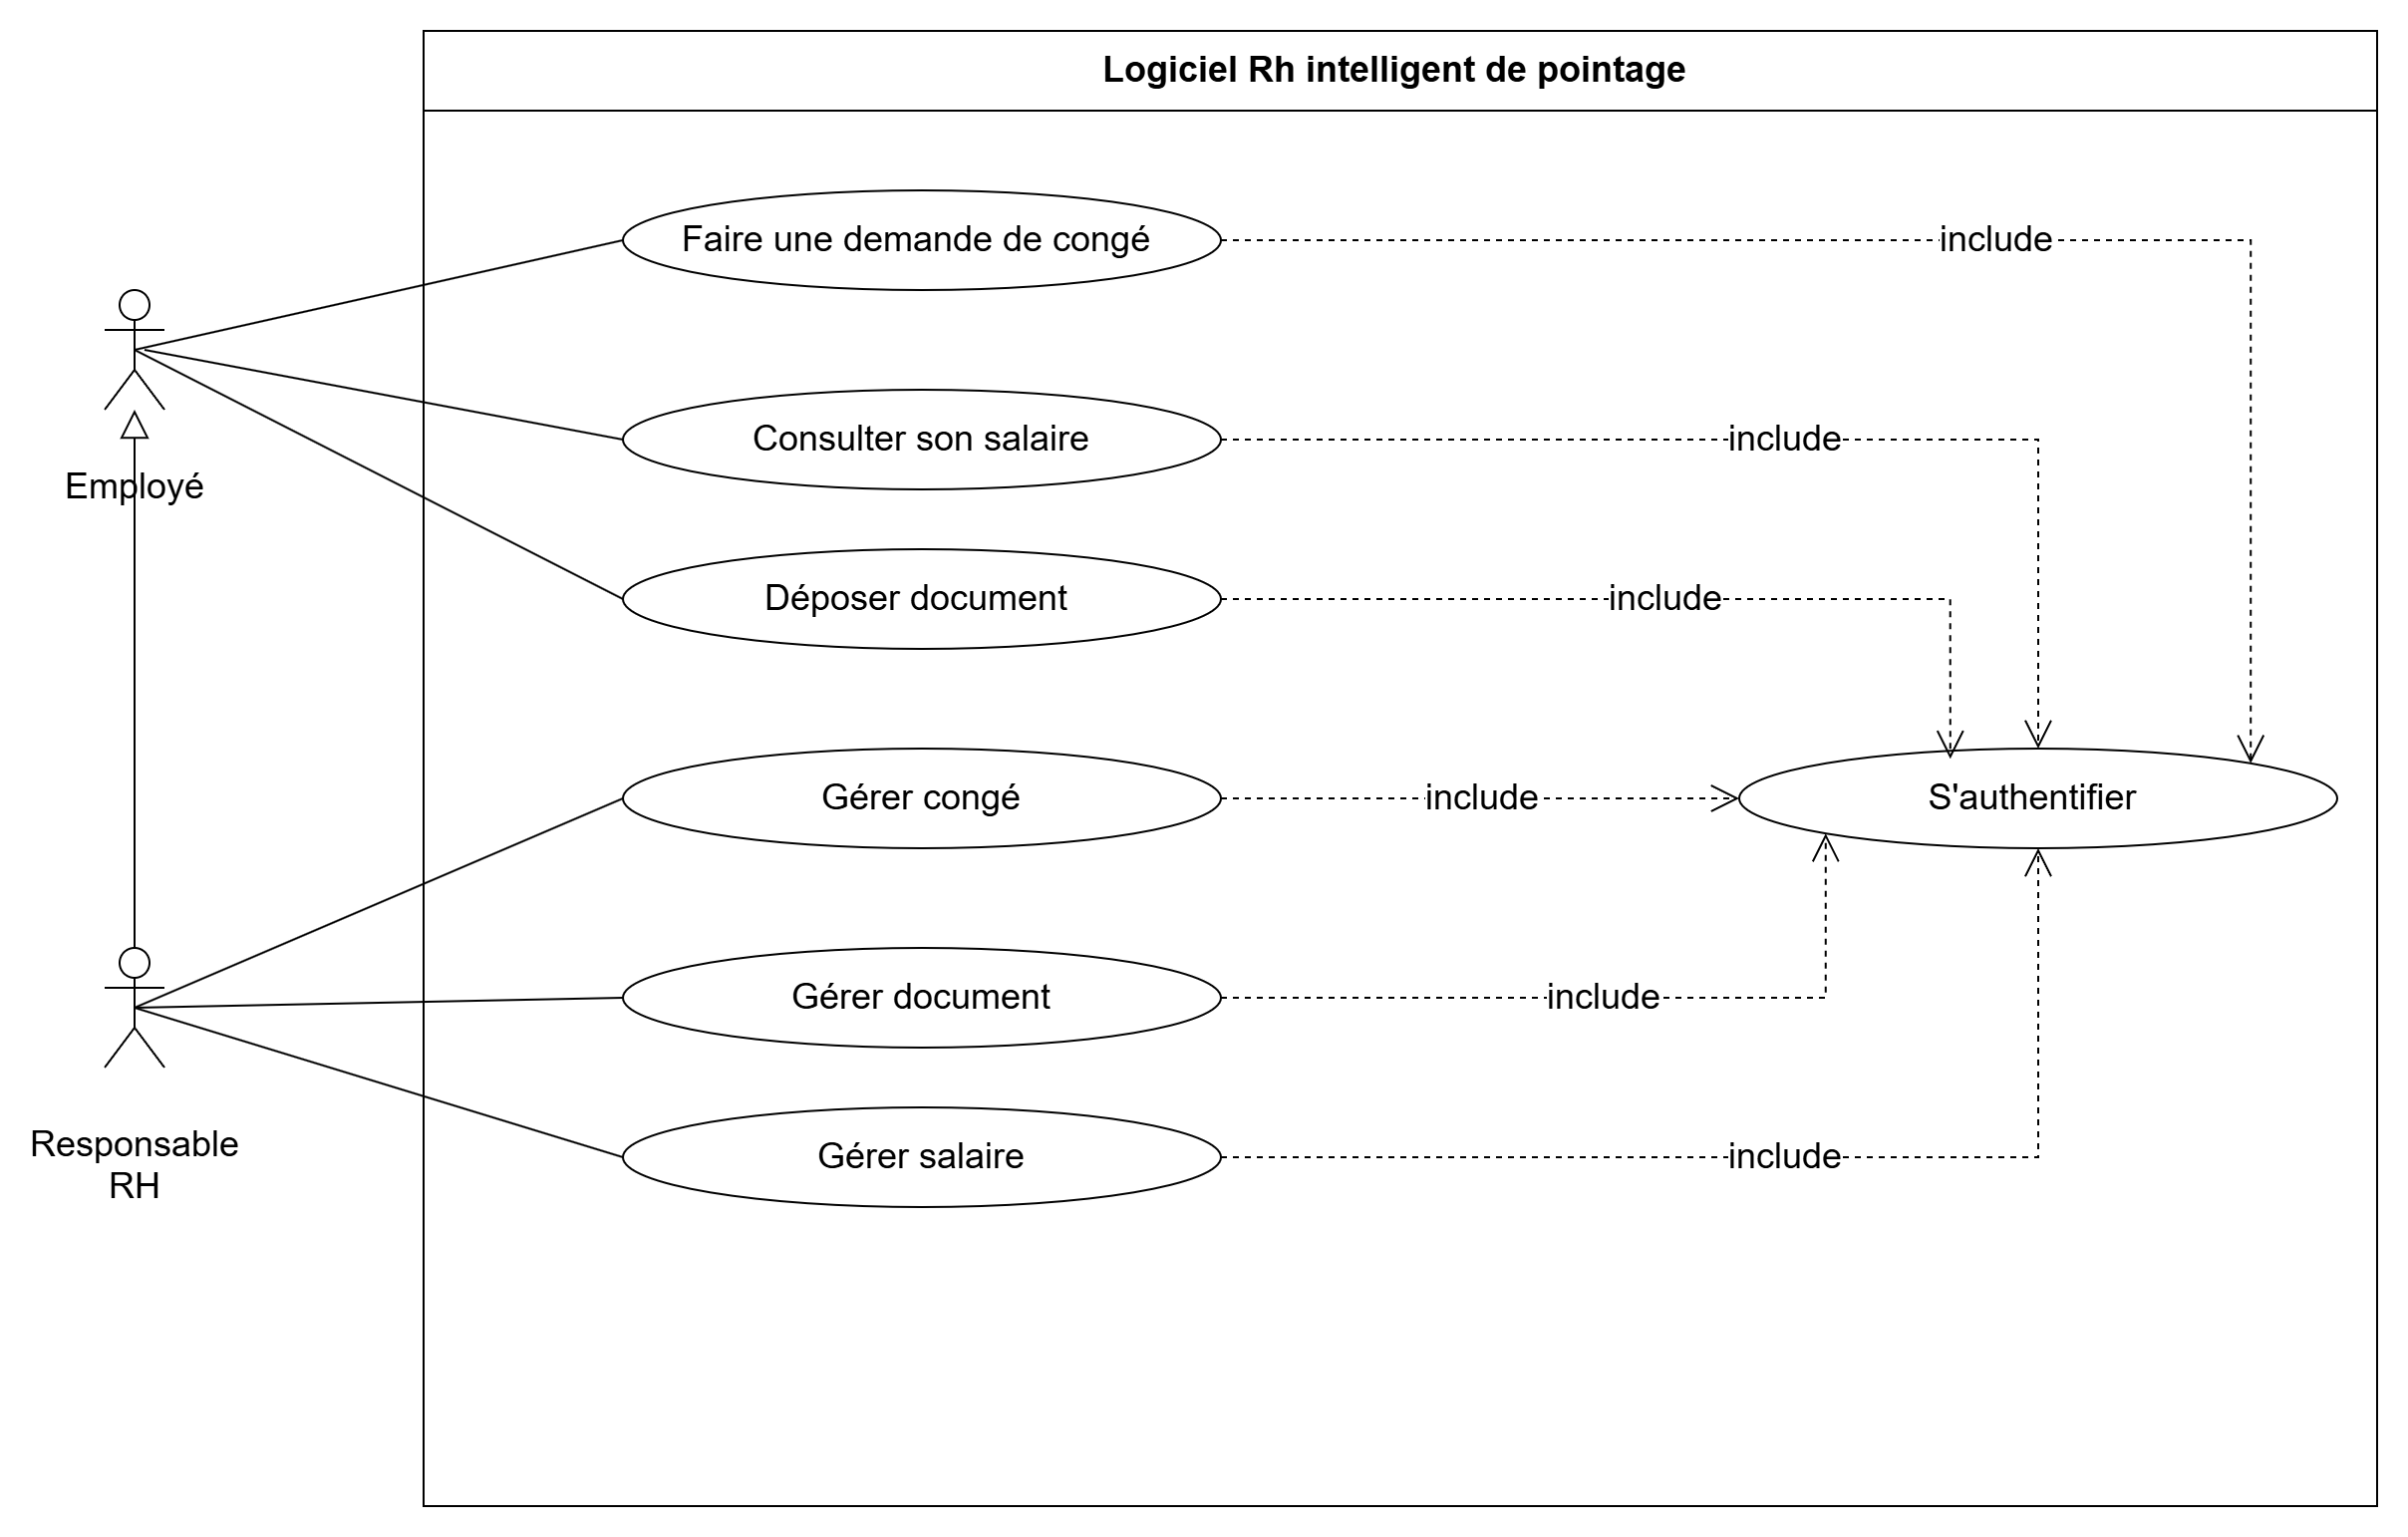
\includegraphics[width=0.9\textwidth]{projet/images/usecase/sprint 3/use_case_s3.png}
    \caption{Diagramme de Cas d'utilisation du Sprint 3}
    \label{fig:usecase_sprint3}
\end{figure}

\item \textbf{Raffinement du cas d'utilisation "Gérer congé"}

\begin{figure}[H]
    \centering
    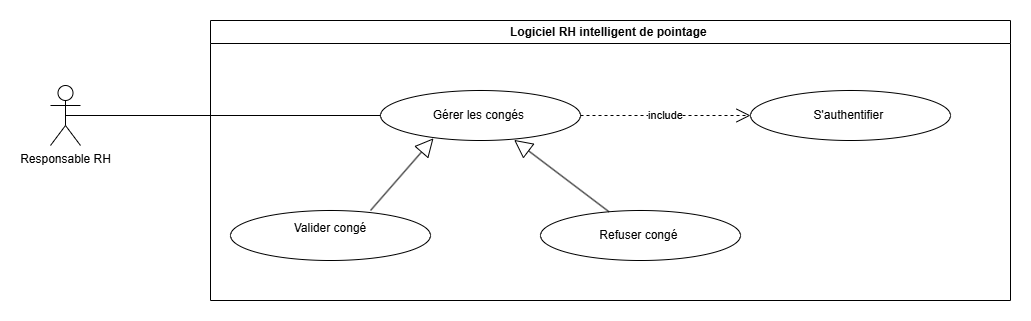
\includegraphics[width=0.9\textwidth]{projet/images/usecase/sprint 3/raffinement_gerer_conges.png}
    \caption{Raffinement du cas d'utilisation "Gérer les congés"}
    \label{fig:raffinement_gerer_conge}
\end{figure}

\item \textbf{Description textuelle : cas d'utilisation «~Valider congé~»}

\begin{center}
\begin{longtable}{|p{5cm}|p{11cm}|}
\hline
\textbf{Nom du cas d'utilisation} & Valider congé \\ \hline
\textbf{Acteurs} & Responsable RH \\ \hline
\textbf{Objectif} & Valider une demande de congé \\ \hline
\textbf{Préconditions} & Le responsable RH doit être authentifié \\ \hline
\textbf{Scénario nominal} &
1. Le responsable RH accède à la liste des demandes. \newline
2. Il sélectionne une demande. \newline
3. Il clique sur "Valider". \newline
4. Le système met à jour le statut de la demande. \\ \hline
\textbf{Scénario d'exception} & Si la demande n'existe pas, le système affiche une erreur. \\ \hline
\textbf{Post-condition} & La demande est validée. \\ \hline
\caption{Description textuelle du cas d'utilisation «~Valider congé~»}
\end{longtable}
\end{center}

\item \textbf{Description textuelle : cas d'utilisation «~Refuser congé~»}

\begin{center}
\begin{longtable}{|p{5cm}|p{11cm}|}
\hline
\textbf{Nom du cas d'utilisation} & Refuser congé \\ \hline
\textbf{Acteurs} & Responsable RH \\ \hline
\textbf{Objectif} & Refuser une demande de congé \\ \hline
\textbf{Préconditions} & Le responsable RH doit être authentifié \\ \hline
\textbf{Scénario nominal} &
1. Le responsable RH accède à la liste des demandes. \newline
2. Il sélectionne une demande. \newline
3. Il clique sur "Refuser". \newline
4. Il saisit un motif. \newline
5. Le système met à jour le statut. \\ \hline
\textbf{Scénario d'exception} & Si aucun motif n'est saisi, le système affiche une erreur. \\ \hline
\textbf{Post-condition} & La demande est refusée. \\ \hline
\caption{Description textuelle du cas d'utilisation «~Refuser congé~»}
\end{longtable}
\end{center}

\item \textbf{Raffinement du cas d'utilisation "Gérer les salaires"}

\begin{figure}[H]
    \centering
    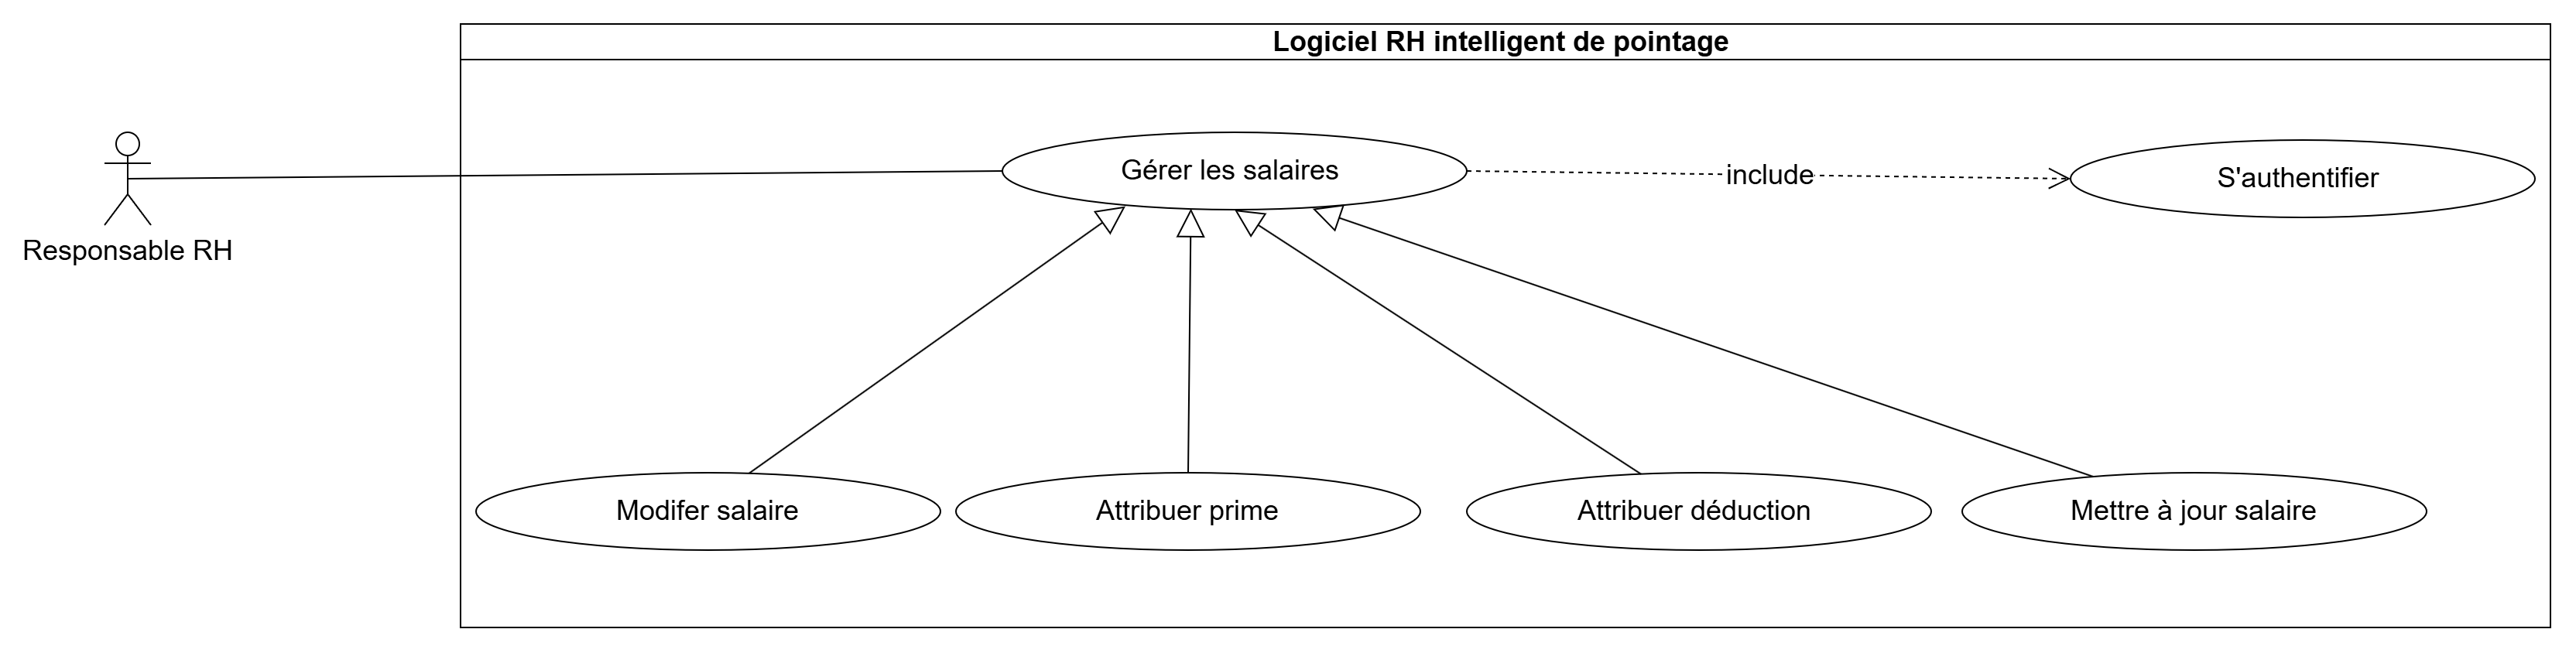
\includegraphics[width=0.9\textwidth]{projet/images/usecase/sprint 3/refinnement_gere_salaire.png}
    \caption{Raffinement du cas d'utilisation "Gérer les salaires"}
    \label{fig:raffinement_gerer_salaires}
\end{figure}

\item \textbf{Description textuelle : cas d'utilisation «~Attribuer déduction~»}

\begin{center}
\begin{longtable}{|p{5cm}|p{11cm}|}
\hline
\textbf{Nom du cas d'utilisation} & Attribuer déduction \\ \hline
\textbf{Acteurs} & Responsable RH \\ \hline
\textbf{Objectif} & Attribuer une déduction à un employé \\ \hline
\textbf{Préconditions} & Responsable RH authentifié \\ \hline
\textbf{Scénario nominal} &
1. Accéder à l'interface de gestion des salaires. \newline
2. Cliquer sur le bouton «~Ajouter une déduction~». \newline
3. Saisir les coordonnées de l'employé (ID ou nom complet). \newline
4. Saisir le montant, le motif et la description de la déduction. \newline
5. Valider l'attribution. \newline
6. Le système enregistre la déduction. \\ \hline
\textbf{Scénario d'exception} & Montant ou raison invalide $\rightarrow$ message d'erreur. \\ \hline
\textbf{Post-condition} & La déduction est attribuée et visible pour l'employé. \\ \hline
\caption{Description textuelle du cas d'utilisation «~Attribuer déduction~»}
\end{longtable}
\end{center}

\item \textbf{Description textuelle : cas d'utilisation «~Attribuer prime~»}

\begin{center}
\begin{longtable}{|p{5cm}|p{11cm}|}
\hline
\textbf{Nom du cas d'utilisation} & Attribuer prime \\ \hline
\textbf{Acteurs} & Responsable RH \\ \hline
\textbf{Objectif} & Attribuer une prime à un employé \\ \hline
\textbf{Préconditions} & Responsable RH authentifié \\ \hline
\textbf{Scénario nominal} &
1. Accéder à l'interface de gestion des salaires. \newline
2. Cliquer sur le bouton «~Ajouter une prime~». \newline
3. Saisir les coordonnées de l'employé (ID ou nom complet). \newline
4. Saisir le montant, le motif et la description de la prime. \newline
5. Valider l'attribution. \newline
6. Le système enregistre la prime. \\ \hline
\textbf{Scénario d'exception} & Montant ou raison invalide $\rightarrow$ message d'erreur. \\ \hline
\textbf{Post-condition} & La prime est attribuée et visible pour l'employé. \\ \hline
\caption{Description textuelle du cas d'utilisation «~Attribuer prime~»}
\end{longtable}
\end{center}



\item \textbf{Description textuelle : cas d'utilisation «~Mettre à jour statut salaire~»}

\begin{center}
\begin{longtable}{|p{5cm}|p{11cm}|}
\hline
\textbf{Nom du cas d'utilisation} & Mettre à jour statut salaire \\ \hline
\textbf{Acteurs} & Responsable RH \\ \hline
\textbf{Objectif} & Mettre à jour le statut du salaire \\ \hline
\textbf{Préconditions} & Responsable RH authentifié \\ \hline
\textbf{Scénario nominal} &
1. Accéder à l'interface de Gestion Salaires. \newline
2. Sélectionner l'employé. \newline
3. Mettre à jour le statut (En Attente / Payé / Traité). \newline
4. Valider la modification. \newline
5. Le système enregistre le nouveau statut. \\ \hline
\textbf{Scénario d'exception} & Informations manquantes $\rightarrow$ message d'erreur. \\ \hline
\textbf{Post-condition} & Le statut du salaire est mis à jour. \\ \hline
\caption{Description textuelle du cas d'utilisation «~Mettre à jour statut salaire~»}
\end{longtable}
\end{center}

\item \textbf{Description textuelle : cas d'utilisation «~Modifier salaire~»}

\begin{center}
\begin{longtable}{|p{5cm}|p{11cm}|}
\hline
\textbf{Nom du cas d'utilisation} & Modifier salaire \\ \hline
\textbf{Acteurs} & Responsable RH \\ \hline
\textbf{Objectif} & Modifier un salaire de base à un employé \\ \hline
\textbf{Préconditions} & Responsable RH authentifié \\ \hline
\textbf{Scénario nominal} &
1. Accéder à l'interface de Gestion Salaires. \newline
2. Sélectionner l'employé. \newline
3. Cliquer sur le bouton modifier. \newline
4. Mettre à jour le salaire. \newline
5. Valider la modification. \newline
6. Le système enregistre le nouveau salaire. \\ \hline
\textbf{Scénario d'exception} & Salaire invalide $\rightarrow$ message d'erreur. \\ \hline
\textbf{Post-condition} & Le salaire est mis à jour. \\ \hline
\caption{Description textuelle du cas d'utilisation «~Modifier salaire~»}
\end{longtable}
\end{center}

\item \textbf{Raffinement du cas d'utilisation "Gérer documents"}

\begin{figure}[H]
    \centering
    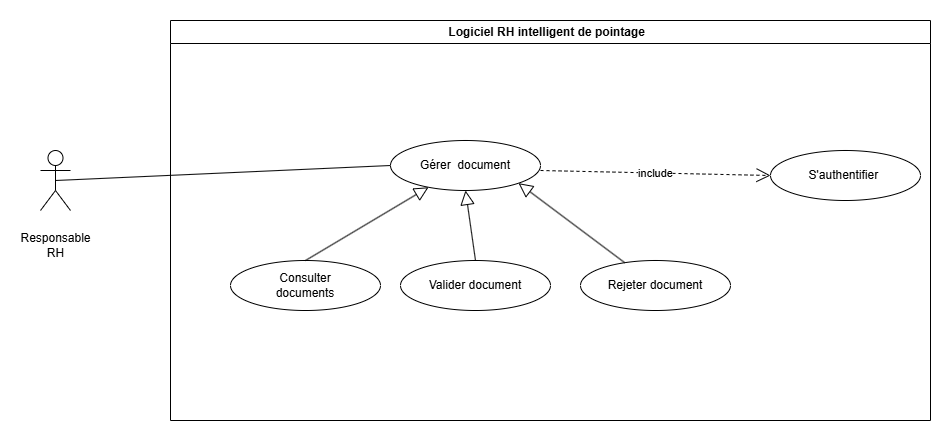
\includegraphics[width=0.9\textwidth]{projet/images/usecase/sprint 3/gerer_document.png}
    \caption{Raffinement du cas d'utilisation "Gérer documents"}
    \label{fig:raffinement_gerer_documents}
\end{figure}

\item \textbf{Description textuelle : cas d'utilisation «~Consulter documents~»}

\begin{center}
\begin{longtable}{|p{5cm}|p{11cm}|}
\hline
\textbf{Nom du cas d'utilisation} & Consulter documents \\ \hline
\textbf{Acteurs} & Responsable RH \\ \hline
\textbf{Objectif} & Consulter les documents envoyés \\ \hline
\textbf{Préconditions} & Responsable RH authentifié \\ \hline
\textbf{Scénario nominal} &
1. Accéder à l'interface des documents. \newline
2. Sélectionner un document. \newline
3. Afficher les détails du document. \\ \hline
\textbf{Scénario d'exception} & Document manquant $\rightarrow$ message "Document non disponible". \\ \hline
\textbf{Post-condition} & Les documents sont consultés. \\ \hline
\caption{Description textuelle du cas d'utilisation «~Consulter documents~»}
\end{longtable}
\end{center}

\item \textbf{Description textuelle : cas d'utilisation «~Valider document~»}

\begin{center}
\begin{longtable}{|p{5cm}|p{11cm}|}
\hline
\textbf{Nom du cas d'utilisation} & Valider document \\ \hline
\textbf{Acteurs} & Responsable RH \\ \hline
\textbf{Objectif} & Approuver un document \\ \hline
\textbf{Préconditions} & Responsable RH authentifié \\ \hline
\textbf{Scénario nominal} &
1. Accéder aux documents. \newline
2. Sélectionner un document. \newline
3. Cliquer sur "Valider". \newline
4. Le système met à jour le statut du document. \\ \hline
\textbf{Scénario d'exception} & Document inexistant $\rightarrow$ message d'erreur. \\ \hline
\textbf{Post-condition} & Document validé. \\ \hline
\caption{Description textuelle du cas d'utilisation «~Valider document~»}
\end{longtable}
\end{center}

\item \textbf{Description textuelle : cas d'utilisation «~Rejeter document~»}

\begin{center}
\begin{longtable}{|p{5cm}|p{11cm}|}
\hline
\textbf{Nom du cas d'utilisation} & Rejeter document \\ \hline
\textbf{Acteurs} & Responsable RH \\ \hline
\textbf{Objectif} & Refuser un document \\ \hline
\textbf{Préconditions} & Responsable RH authentifié \\ \hline
\textbf{Scénario nominal} &
1. Accéder aux documents. \newline
2. Sélectionner un document. \newline
3. Cliquer sur "Rejeter". \newline
4. Le système met à jour le statut. \\ \hline
\textbf{Scénario d'exception} & Document inexistant $\rightarrow$ message d'erreur. \\ \hline
\textbf{Post-condition} & Document rejeté. \\ \hline
\caption{Description textuelle du cas d'utilisation «~Rejeter document~»}
\end{longtable}
\end{center}

\item \textbf{Raffinement du cas d'utilisation "Consulter  son salaire"}

\begin{figure}[H]
    \centering
    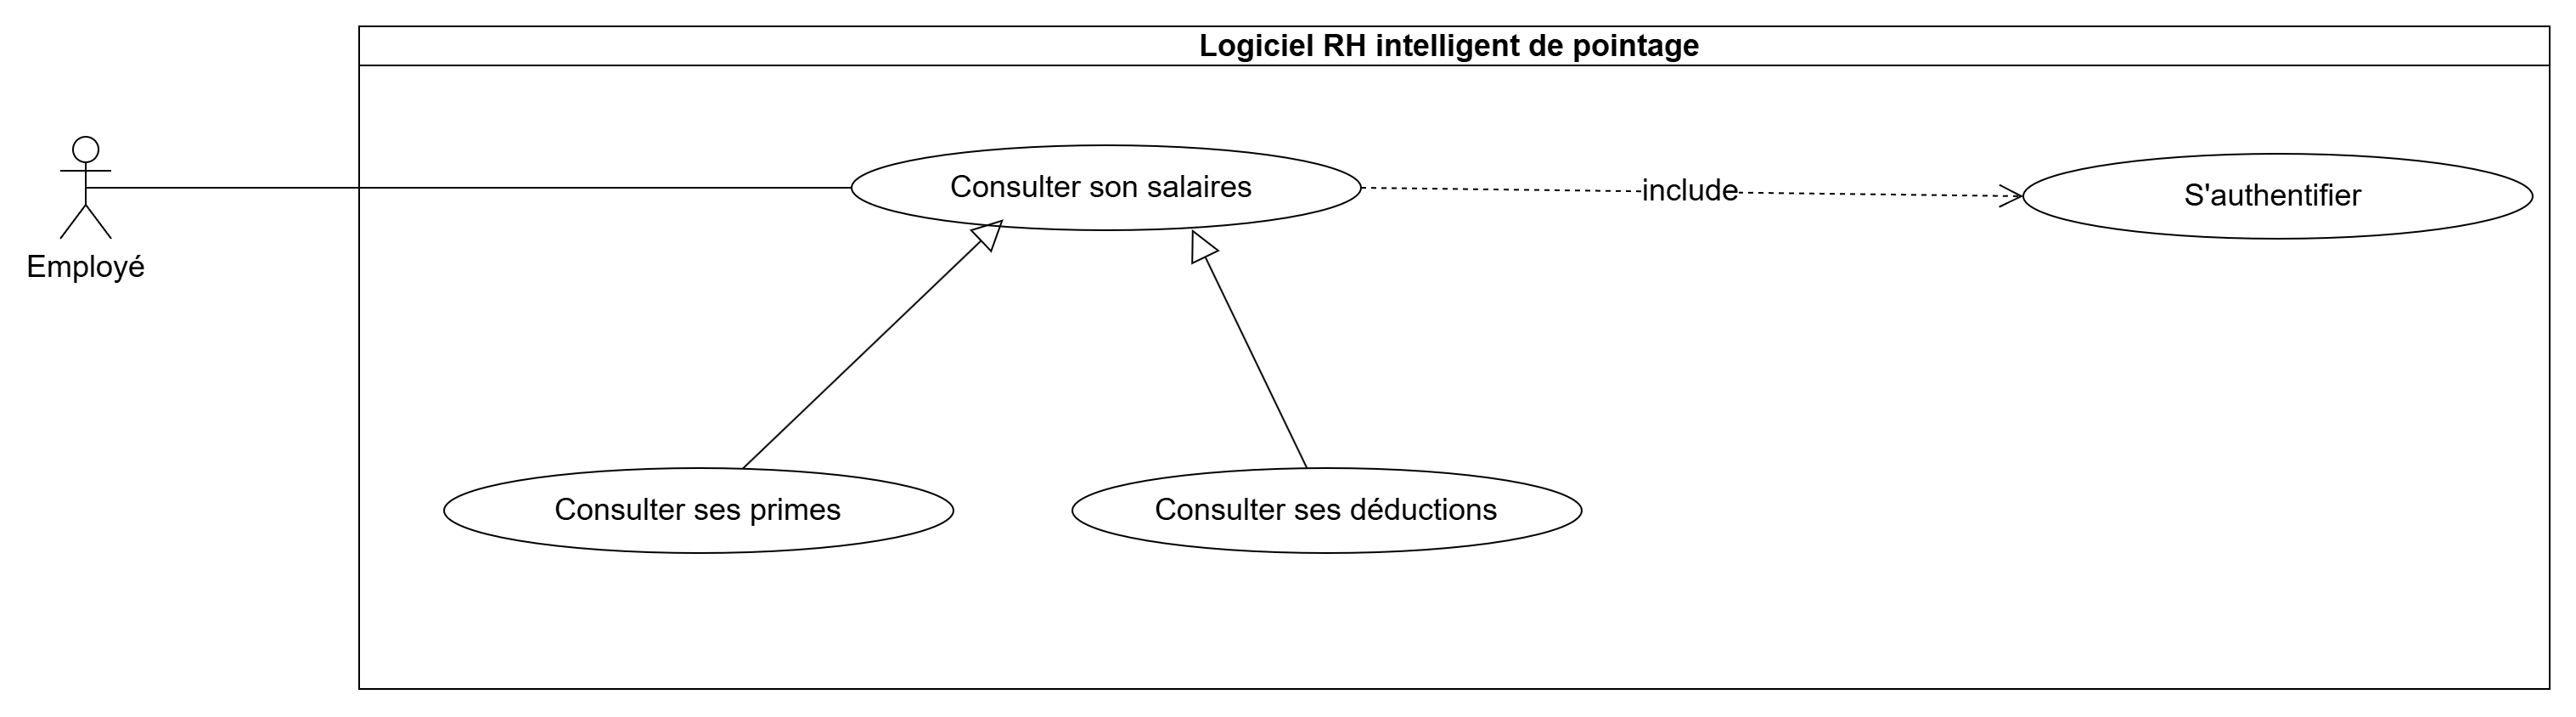
\includegraphics[width=0.9\textwidth]{projet/images/usecase/sprint 3/CS.png}
    \caption{Raffinement du cas d'utilisation "Gérer les salaires"}
    \label{fig:raffinement_gerer_salaires}
\end{figure}
\item \textbf{Description textuelle : cas d'utilisation «~Consulter primes~»}

\begin{center}
\begin{longtable}{|p{5cm}|p{11cm}|}
\hline
\textbf{Nom du cas d'utilisation} & Consulter primes \\ \hline
\textbf{Acteurs} & Employé \\ \hline
\textbf{Objectif} & Consulter mes primes \\ \hline
\textbf{Préconditions} & Employé authentifié \\ \hline
\textbf{Scénario nominal} &
1. Accéder à l'interface de Mon Salaire. \newline
2. Cliquer sur "Cliquer pour consulter primes". \newline
3. Affichage des primes et montants. \\ \hline
\textbf{Scénario d'exception} & Aucune prime $\rightarrow$ message "Aucune prime disponible". \\ \hline
\textbf{Post-condition} & L'employé visualise ses primes. \\ \hline
\caption{Description textuelle du cas d'utilisation «~Consulter primes~»}
\end{longtable}
\end{center}

\item \textbf{Description textuelle : cas d'utilisation «~Consulter déductions~»}

\begin{center}
\begin{longtable}{|p{5cm}|p{11cm}|}
\hline
\textbf{Nom du cas d'utilisation} & Consulter déductions \\ \hline
\textbf{Acteurs} & Employé \\ \hline
\textbf{Objectif} & Consulter mes déductions \\ \hline
\textbf{Préconditions} & Employé authentifié \\ \hline
\textbf{Scénario nominal} &
1. Accéder à l'interface de Mon Salaire. \newline
2. Cliquer sur "Cliquer pour consulter déductions". \newline
3. Affichage des déductions et montants. \\ \hline
\textbf{Scénario d'exception} & Aucune déduction $\rightarrow$ message "Aucune déduction disponible". \\ \hline
\textbf{Post-condition} & L'employé visualise ses déductions. \\ \hline
\caption{Description textuelle du cas d'utilisation «~Consulter déductions~»}
\end{longtable}
\end{center}

\item \textbf{Description textuelle : cas d'utilisation «~Consulter salaire~»}

\begin{center}
\begin{longtable}{|p{5cm}|p{11cm}|}
\hline
\textbf{Nom du cas d'utilisation} & Consulter statut du salaire \\ \hline
\textbf{Acteurs} & Employé \\ \hline
\textbf{Objectif} & Voir le statut du salaire \\ \hline
\textbf{Préconditions} & Employé authentifié \\ \hline
\textbf{Scénario nominal} &
1. Accéder à l'interface de Mon Salaire. \newline
2. Voir Historique des Paiements. \newline
3. Affichage du statut (versé ou non). \\ \hline
\textbf{Scénario d'exception} & Informations manquantes $\rightarrow$ message "Information non disponible". \\ \hline
\textbf{Post-condition} & L'employé connaît le statut de son salaire. \\ \hline
\caption{Description textuelle du cas d'utilisation «~Consulter statut du salaire~»}
\end{longtable}
\end{center}

\item \textbf{Description textuelle : cas d'utilisation «~Demander un congé~»}

\begin{center}
\begin{longtable}{|p{5cm}|p{11cm}|}
\hline
\textbf{Nom du cas d'utilisation} & Demander un congé \\ \hline
\textbf{Acteurs} & Employé \\ \hline
\textbf{Objectif} & Envoyer une demande de congé \\ \hline
\textbf{Préconditions} & Employé authentifié \\ \hline
\textbf{Scénario nominal} &
1. Accéder à l'interface de demande de congé. \newline
2. Cliquer sur "Demander un congé". \newline
3. Saisir date début, date fin et motif. \newline
4. Valider la demande. \newline
5. Le système enregistre et envoie au RH. \\ \hline
\textbf{Scénario d'exception} & Champs vides ou dates incorrectes $\rightarrow$ message d'erreur. \\ \hline
\textbf{Post-condition} & Demande enregistrée et en attente de validation. \\ \hline
\caption{Description textuelle du cas d'utilisation «~Demander un congé~»}
\end{longtable}
\end{center}

\item \textbf{Description textuelle : cas d'utilisation «~Déposer document~»}

\begin{center}
\begin{longtable}{|p{5cm}|p{11cm}|}
\hline
\textbf{Nom du cas d'utilisation} & Déposer document \\ \hline
\textbf{Acteurs} & Employé \\ \hline
\textbf{Objectif} & Déposer un document \\ \hline
\textbf{Préconditions} & Employé authentifié \\ \hline
\textbf{Scénario nominal} &
1. Accéder à l'espace personnel. \newline
2. Cliquer sur "Déposer document". \newline
3. Sélectionner le fichier et saisir les infos. \newline
4. Valider l'envoi. \newline
5. Le système enregistre et notifie le RH. \\ \hline
\textbf{Scénario d'exception} & Fichier invalide ou manquant $\rightarrow$ message d'erreur. \\ \hline
\textbf{Post-condition} & Document enregistré et accessible au RH. \\ \hline
\caption{Description textuelle du cas d'utilisation «~Déposer document~»}
\end{longtable}
\end{center}

\end{itemize}

\subsection{Conception}
Cette section présente les différents diagrammes UML réalisés afin de modéliser le fonctionnement du système, notamment les diagrammes de séquence et les diagrammes de classes, permettant de décrire les interactions entre les acteurs ainsi que la structure globale de l'application.

\subsubsection{Diagramme de séquence du sprint 3}

\begin{itemize}

\item[$\bullet$] \textbf{Diagramme de séquence du cas d'utilisation «~Valider congé~»}

Ce diagramme illustre la validation d'une demande de congé par le Responsable RH. Il consulte la liste des demandes en attente, sélectionne celle à traiter et le système met à jour son statut en approuvé et notifie l'employé concerné.

\begin{figure}[H]
    \centering
    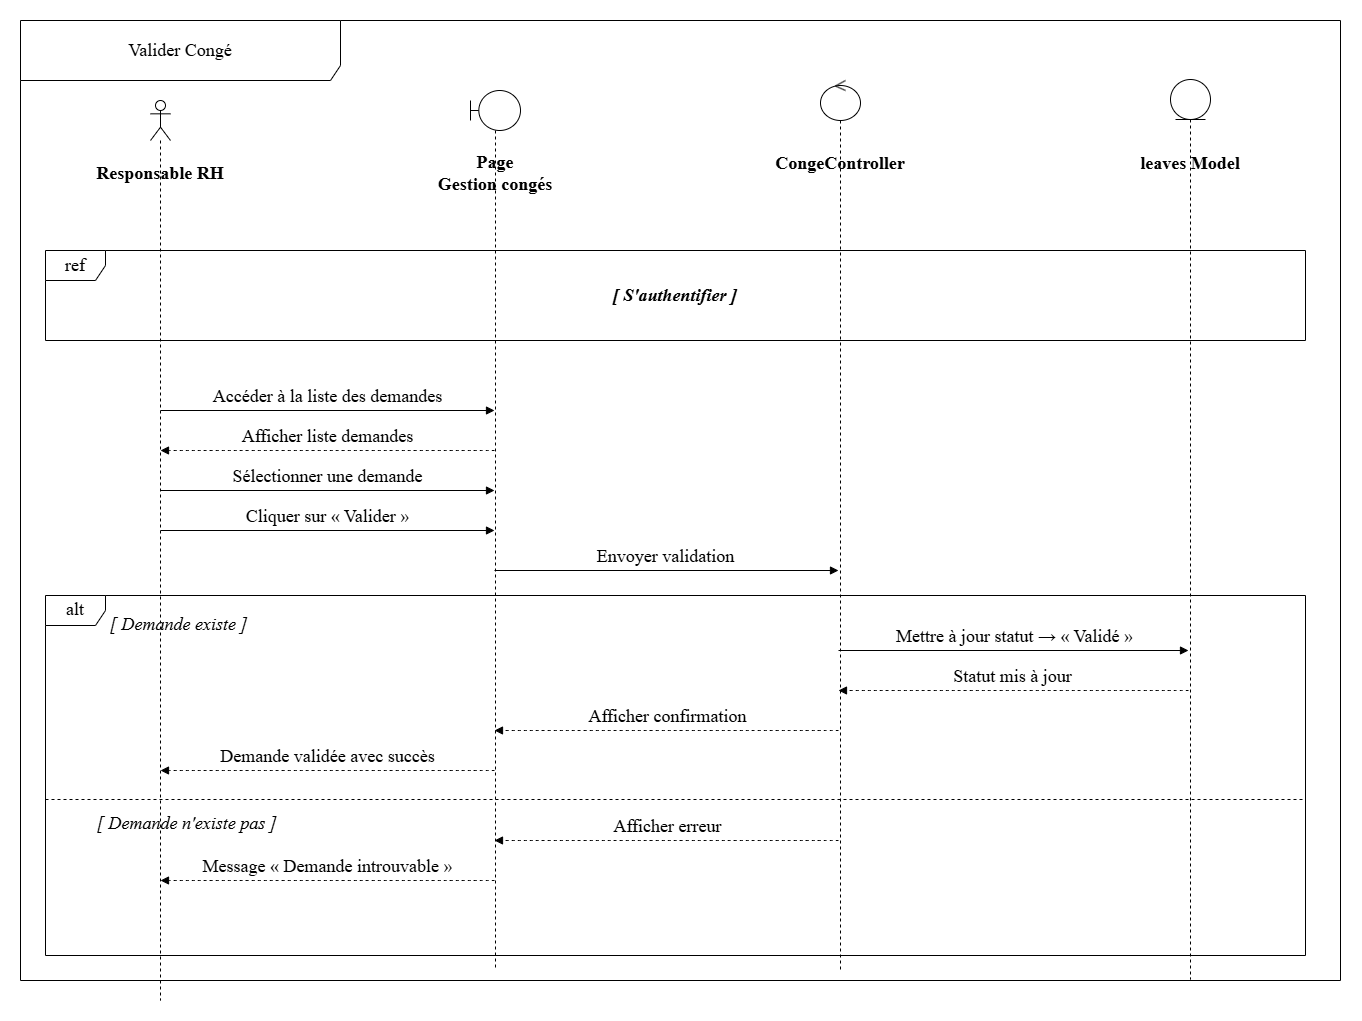
\includegraphics[width=0.9\textwidth]{projet/images/sequence s3/valider conger.drawio.png}
    \caption{Diagramme de séquence du cas d'utilisation «~Valider congé~»}
\end{figure}

\item[$\bullet$] \textbf{Diagramme de séquence du cas d'utilisation «~Refuser congé~»}

Ce diagramme décrit le refus d'une demande de congé par le Responsable RH. Après sélection de la demande, il saisit un motif de refus obligatoire et le système met à jour le statut en refusé avant de notifier l'employé.

\begin{figure}[H]
    \centering
    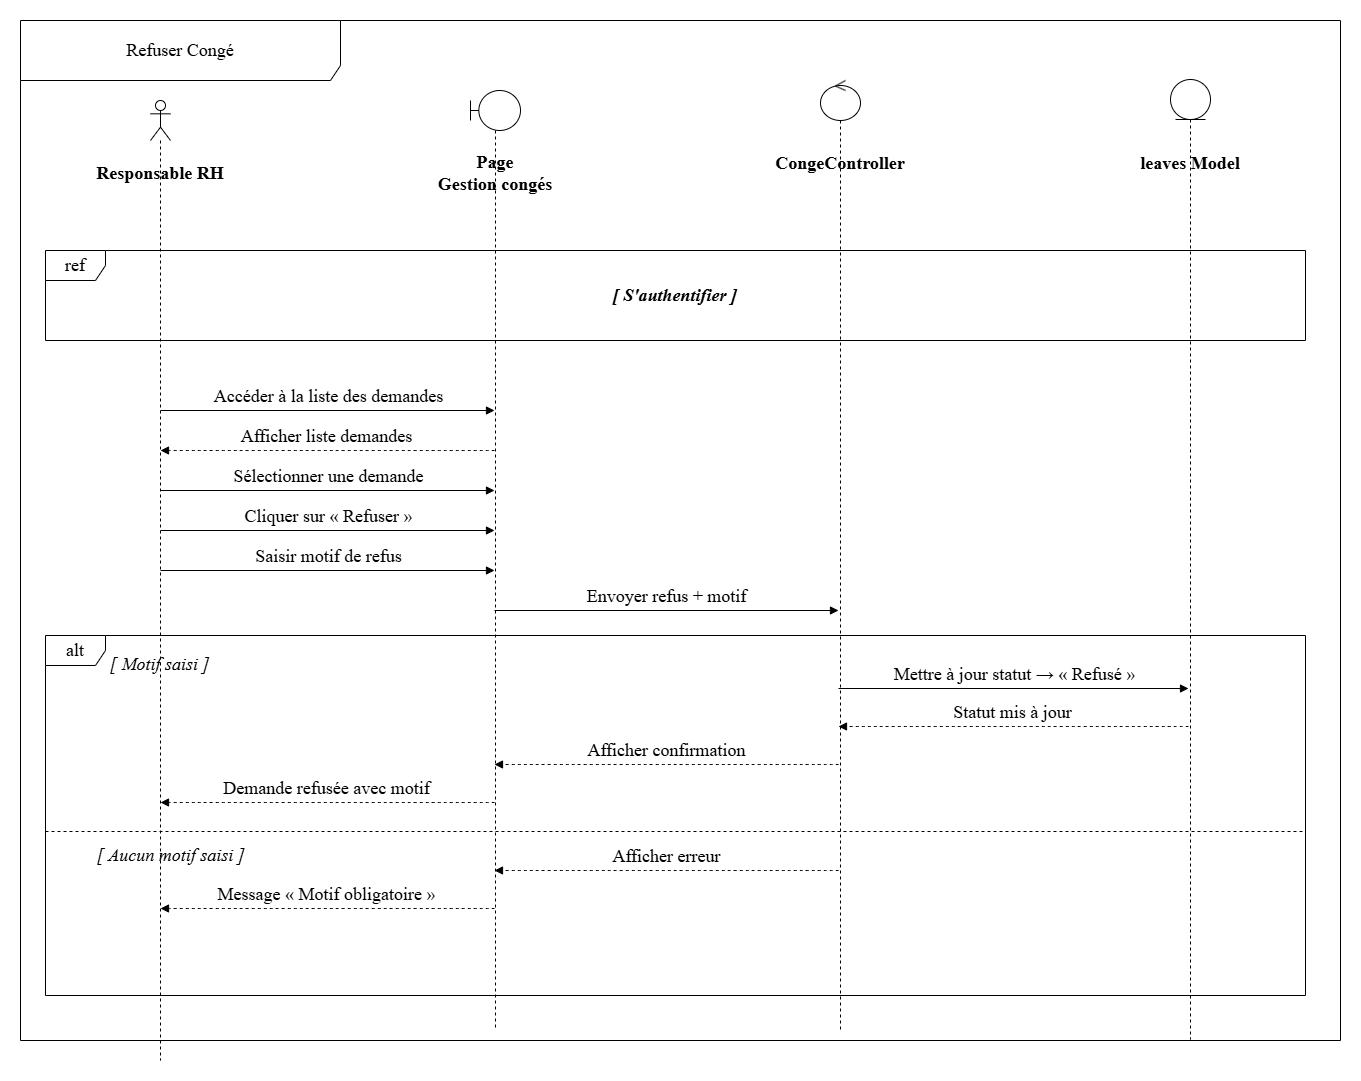
\includegraphics[width=0.9\textwidth]{projet/images/sequence s3/refuser conges.drawio.png}
    \caption{Diagramme de séquence du cas d'utilisation «~Refuser congé~»}
\end{figure}

\item[$\bullet$] \textbf{Diagramme de séquence du cas d'utilisation «~Attribuer prime~»}

Ce diagramme présente l'attribution d'une prime à un employé par le Responsable RH. Il sélectionne l'employé, saisit le montant et la raison de la prime, et le système enregistre l'opération qui devient alors consultable par l'employé concerné.

\begin{figure}[H]
    \centering
    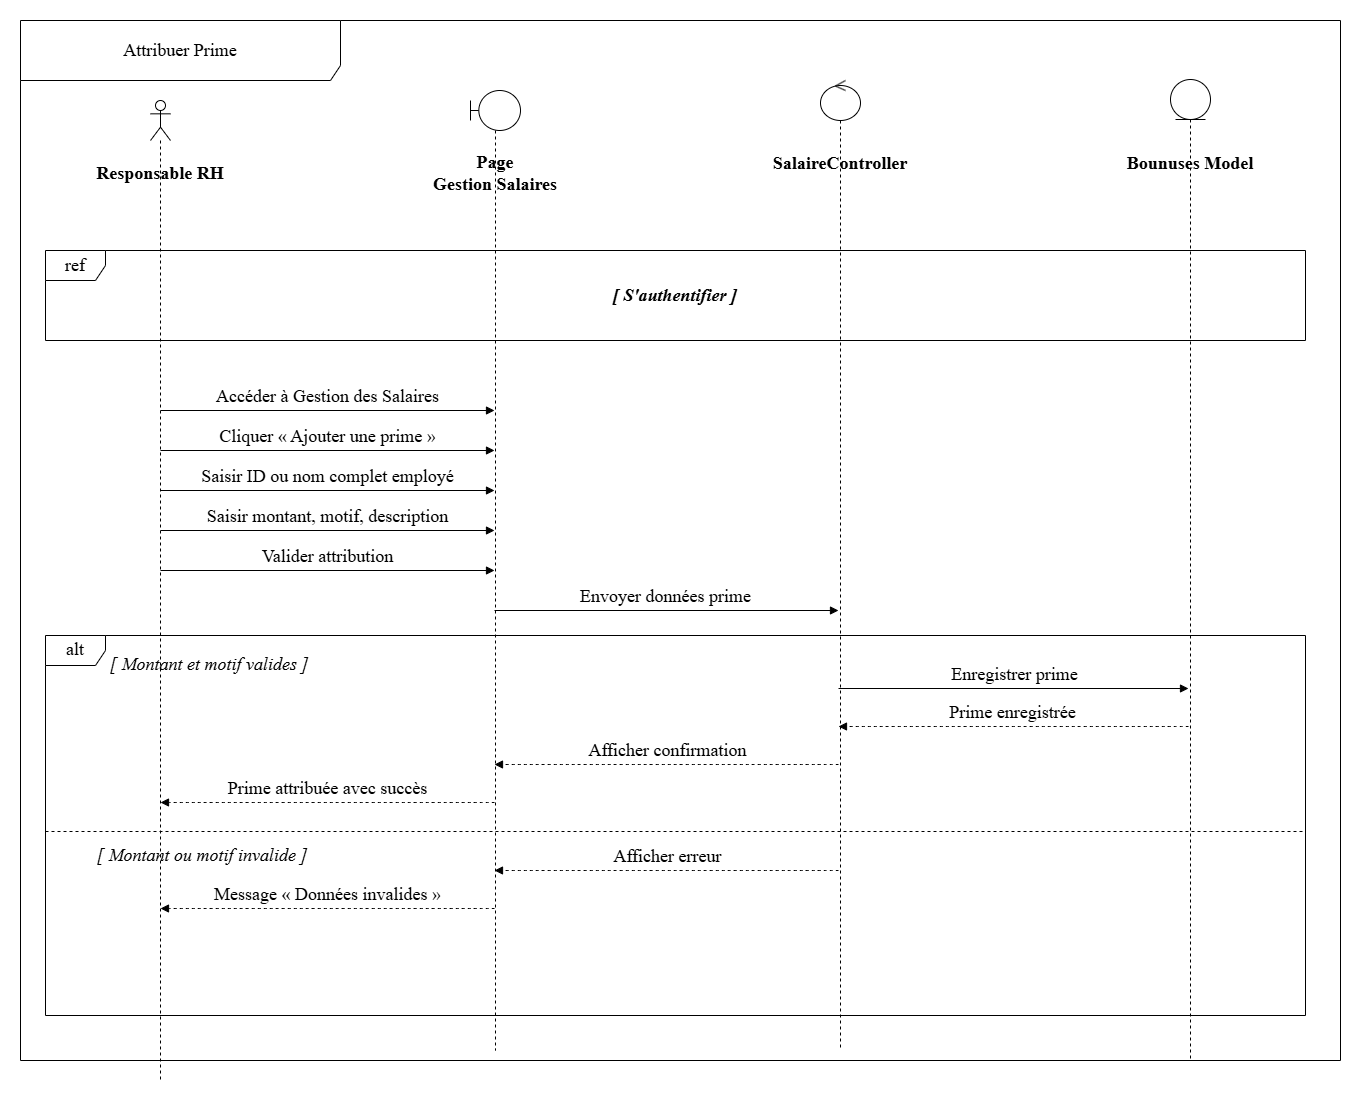
\includegraphics[width=0.9\textwidth]{projet/images/sequence s3/attribuer bounuses.drawio.png}
    \caption{Diagramme de séquence du cas d'utilisation «~Attribuer prime~»}
\end{figure}

\item[$\bullet$] \textbf{Diagramme de séquence du cas d'utilisation «~Attribuer déduction~»}

Ce diagramme illustre l'application d'une déduction sur le salaire d'un employé par le Responsable RH. Il sélectionne l'employé, saisit le montant et le motif de la déduction, et le système enregistre l'opération pour qu'elle soit reflétée dans la fiche de paie.

\begin{figure}[H]
    \centering
    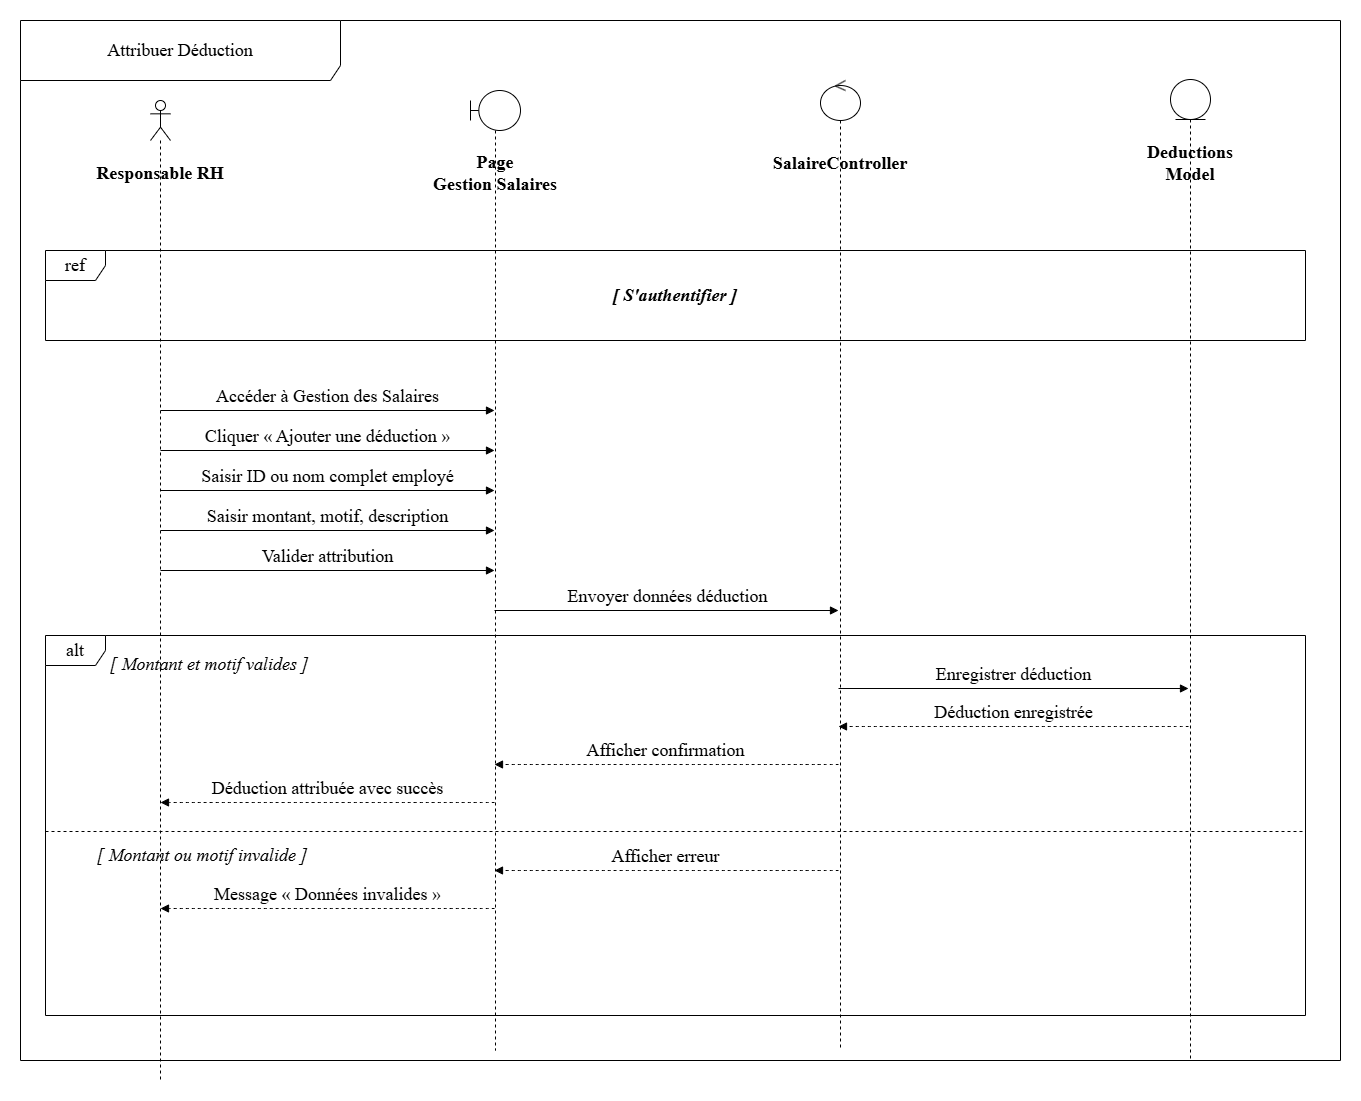
\includegraphics[width=0.9\textwidth]{projet/images/sequence s3/attribuer deduction.drawio.png}
    \caption{Diagramme de séquence du cas d'utilisation «~Attribuer déductions~»}
\end{figure}

\item[$\bullet$] \textbf{Diagramme de séquence du cas d'utilisation «~Mettre à jour statut salaire~»}

Ce diagramme décrit la mise à jour du statut de paiement du salaire d'un employé par le Responsable RH. Il sélectionne l'employé, choisit le nouveau statut (versé ou non versé) et le système enregistre la modification pour la rendre visible à l'employé.

\begin{figure}[H]
    \centering
    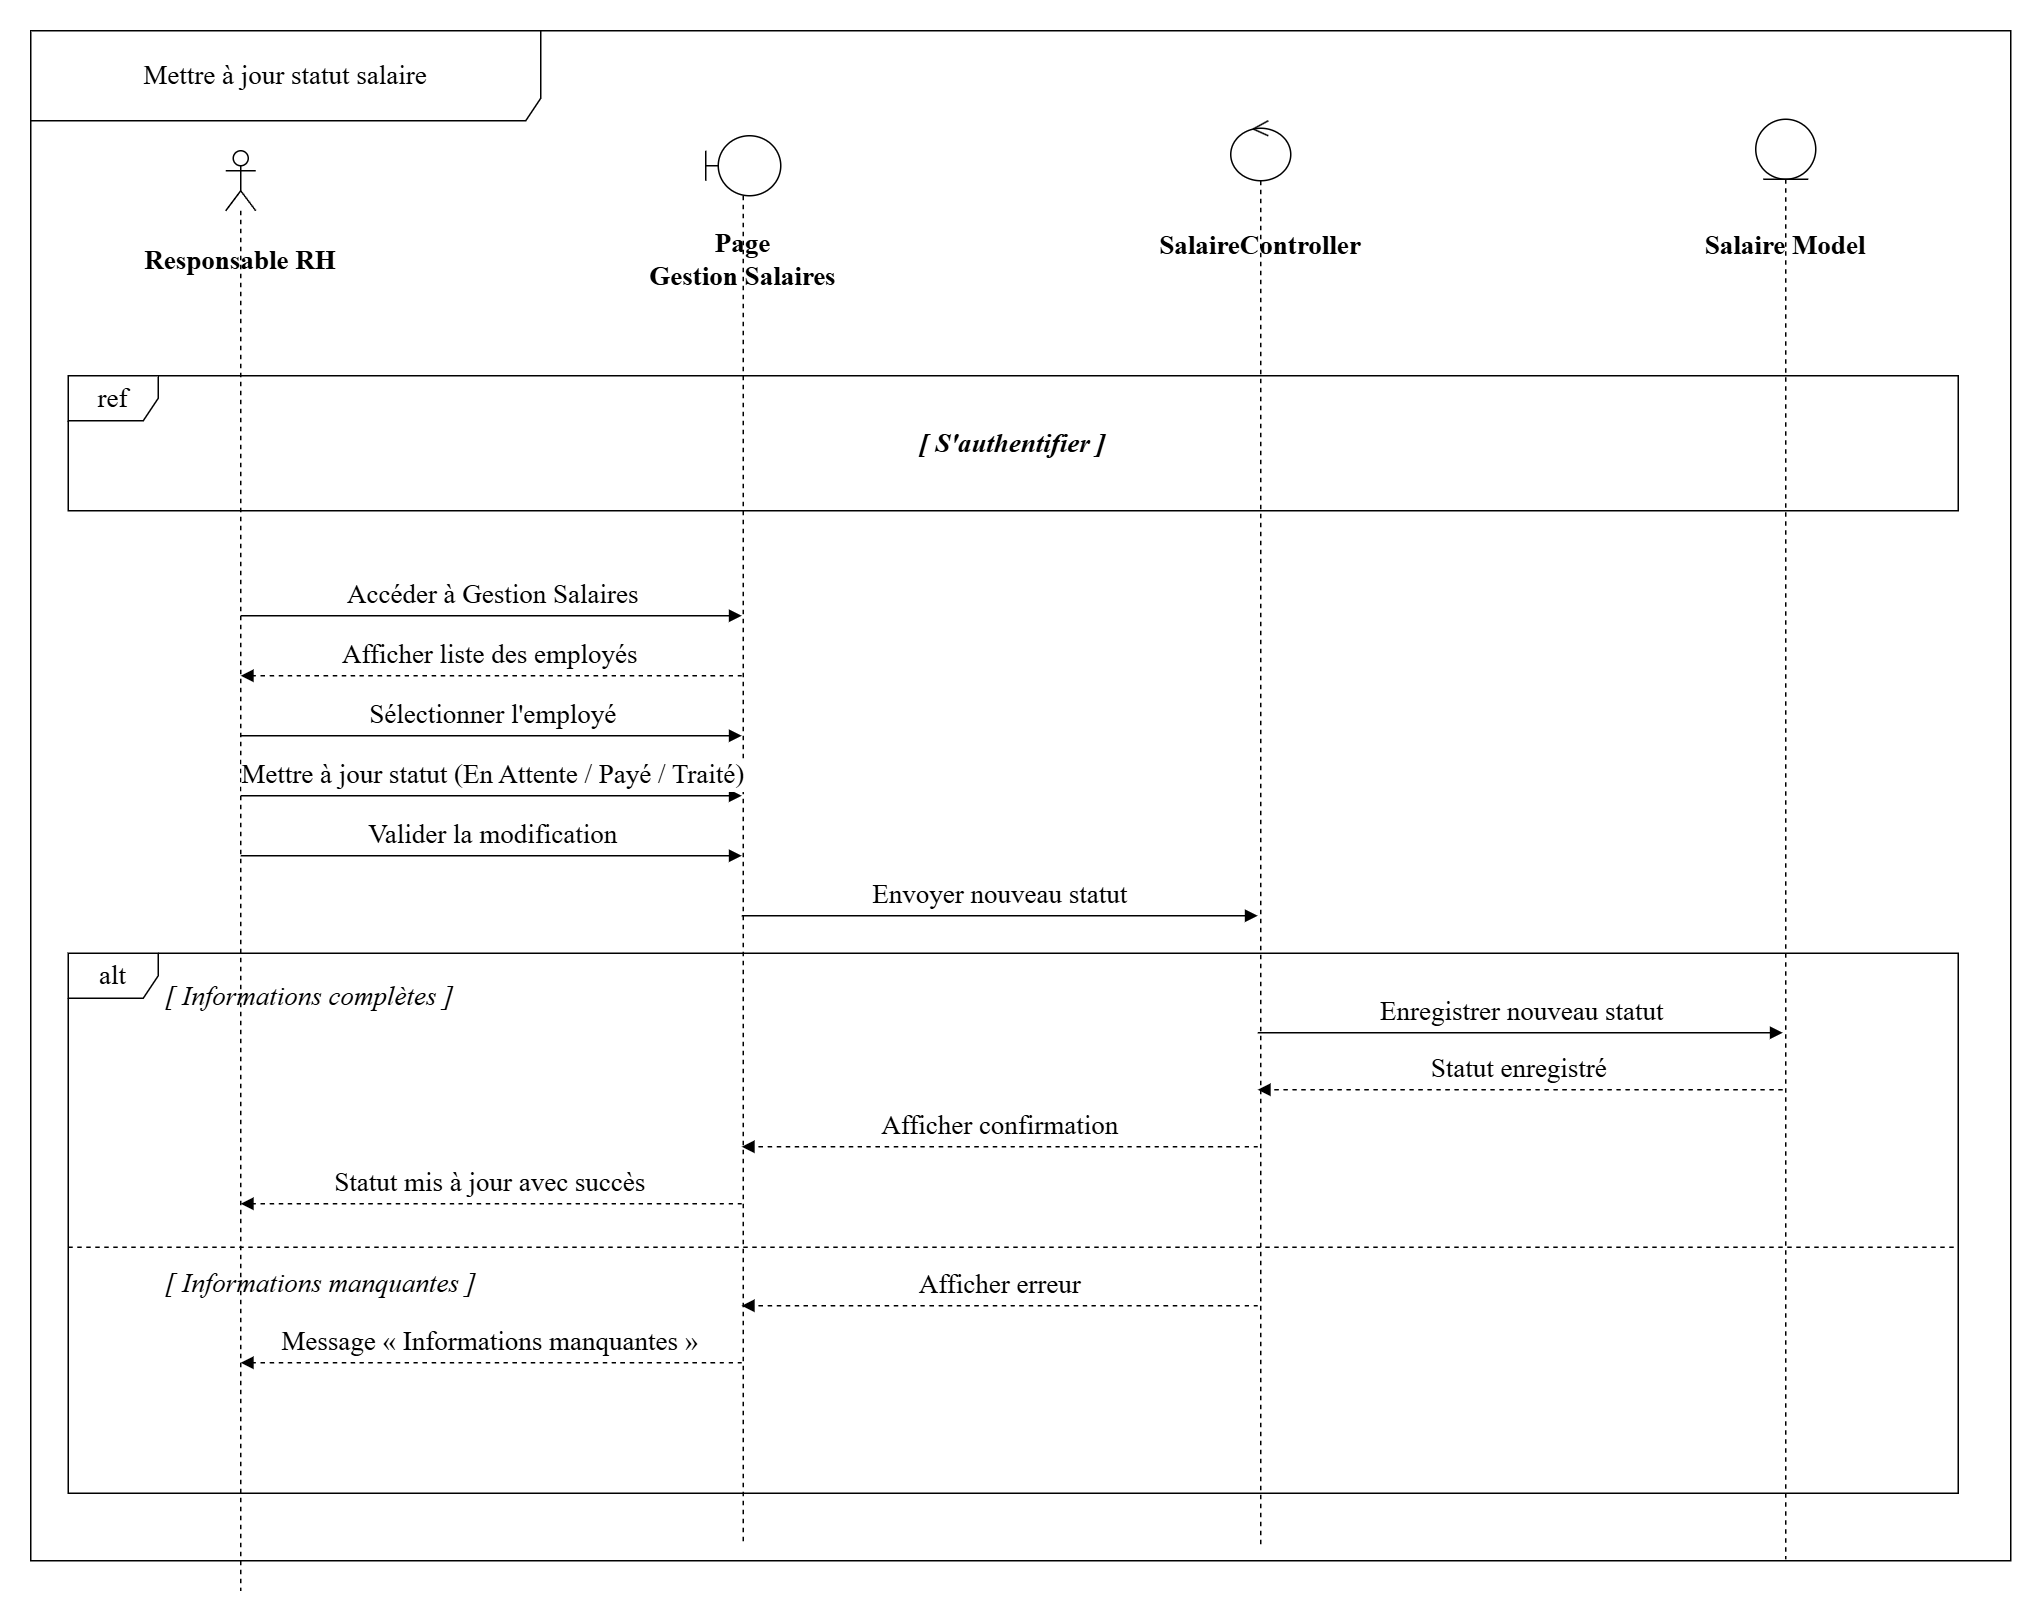
\includegraphics[width=0.9\textwidth]{projet/images/sequence s3/mis_ajour_salaire.png}
    \caption{Diagramme de séquence du cas d'utilisation «~Mettre à jour statut salaire~»}
\end{figure}

\item[$\bullet$] \textbf{Diagramme de séquence du cas d'utilisation «~Modifier salaire~»}

Ce diagramme décrit la mise à jour du statut de paiement du salaire d'un employé par le Responsable RH. Il sélectionne l'employé, choisit le nouveau statut (versé ou non versé) et le système enregistre la modification pour la rendre visible à l'employé.

\begin{figure}[H]
    \centering
    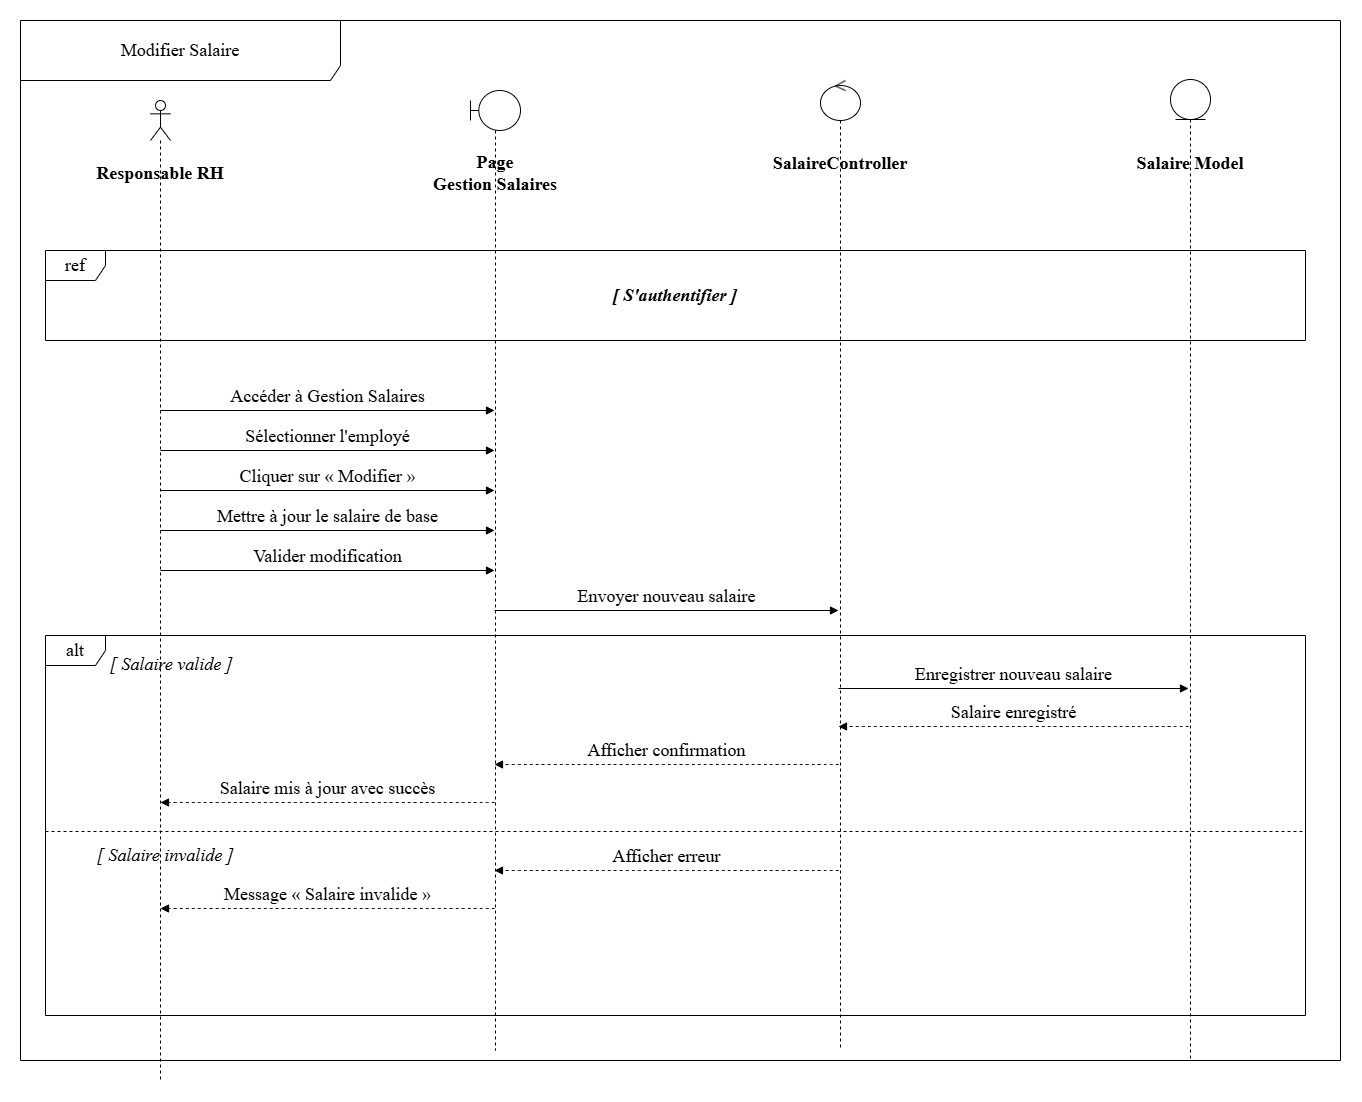
\includegraphics[width=0.9\textwidth]{projet/images/sequence s3/Modifier salaire.drawio.png}
    \caption{Diagramme de séquence du cas d'utilisation «~Modifier salaire~»}
\end{figure}

\item[$\bullet$] \textbf{Diagramme de séquence du cas d'utilisation «~Consulter documents~»}

Ce diagramme présente la consultation des documents soumis par les employés. Le Responsable RH accède à l'interface des documents, sélectionne un document et le système affiche ses détails ou indique son indisponibilité.

\begin{figure}[H]
    \centering
    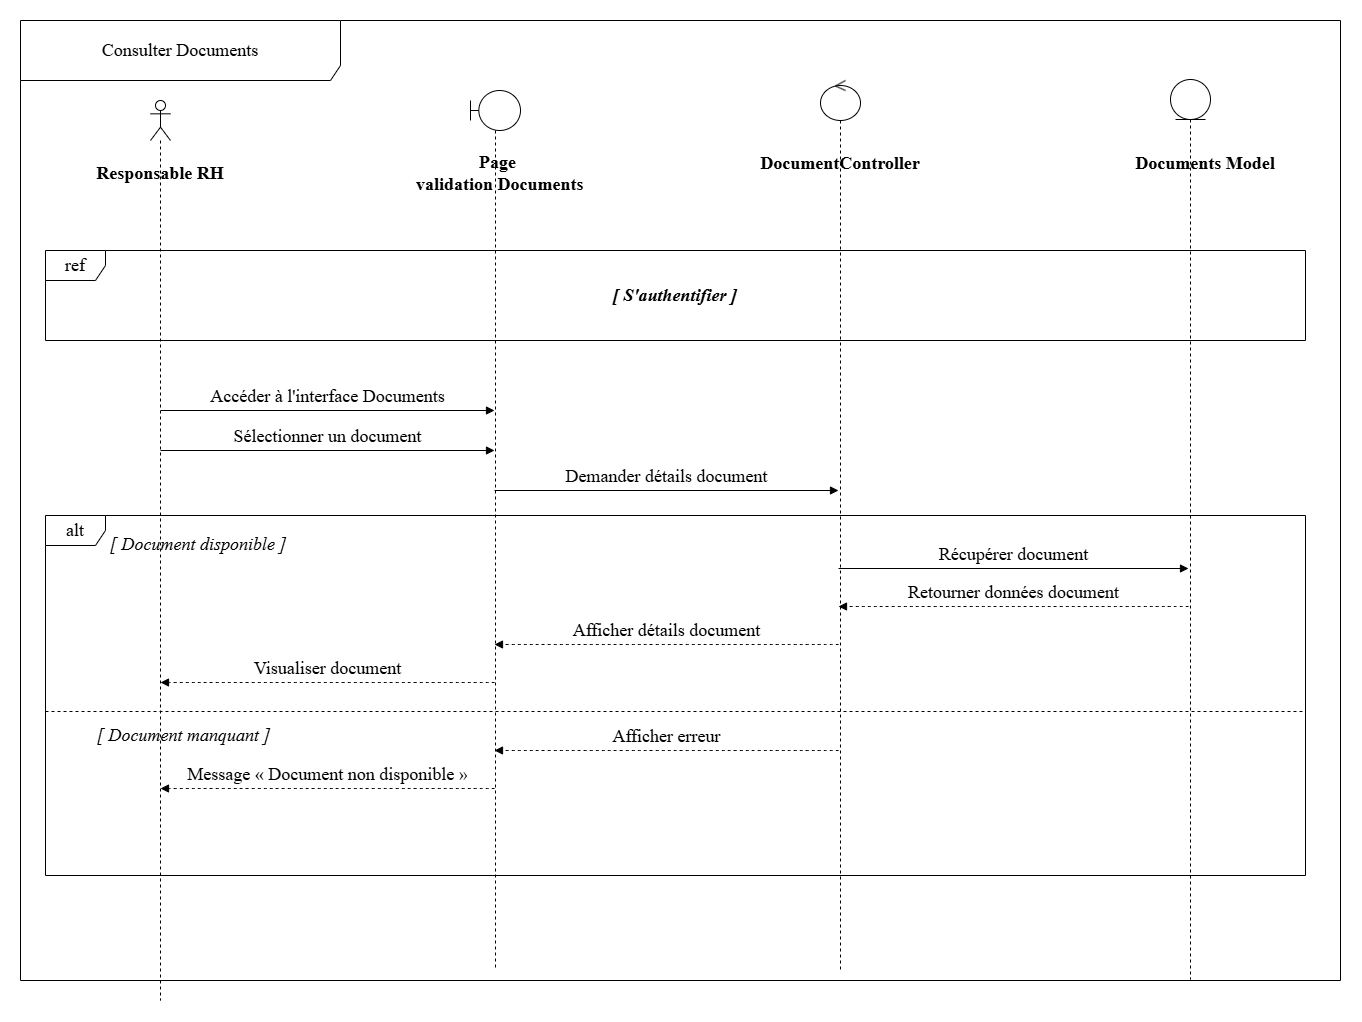
\includegraphics[width=0.9\textwidth]{projet/images/sequence s3/_consulter documents.drawio.png}
    \caption{Diagramme de séquence du cas d'utilisation «~Consulter documents~»}
\end{figure}

\item[$\bullet$] \textbf{Diagramme de séquence du cas d'utilisation «~Valider ou Rejeter document~»}

Ce diagramme illustre la validation ou le rejet d'un document soumis par un employé. Le Responsable RH sélectionne le document, clique sur valider ou rejeter et le système met à jour son statut en approuvé, le rendant officiellement accepté dans le dossier de l'employé.

\begin{figure}[H]
    \centering
    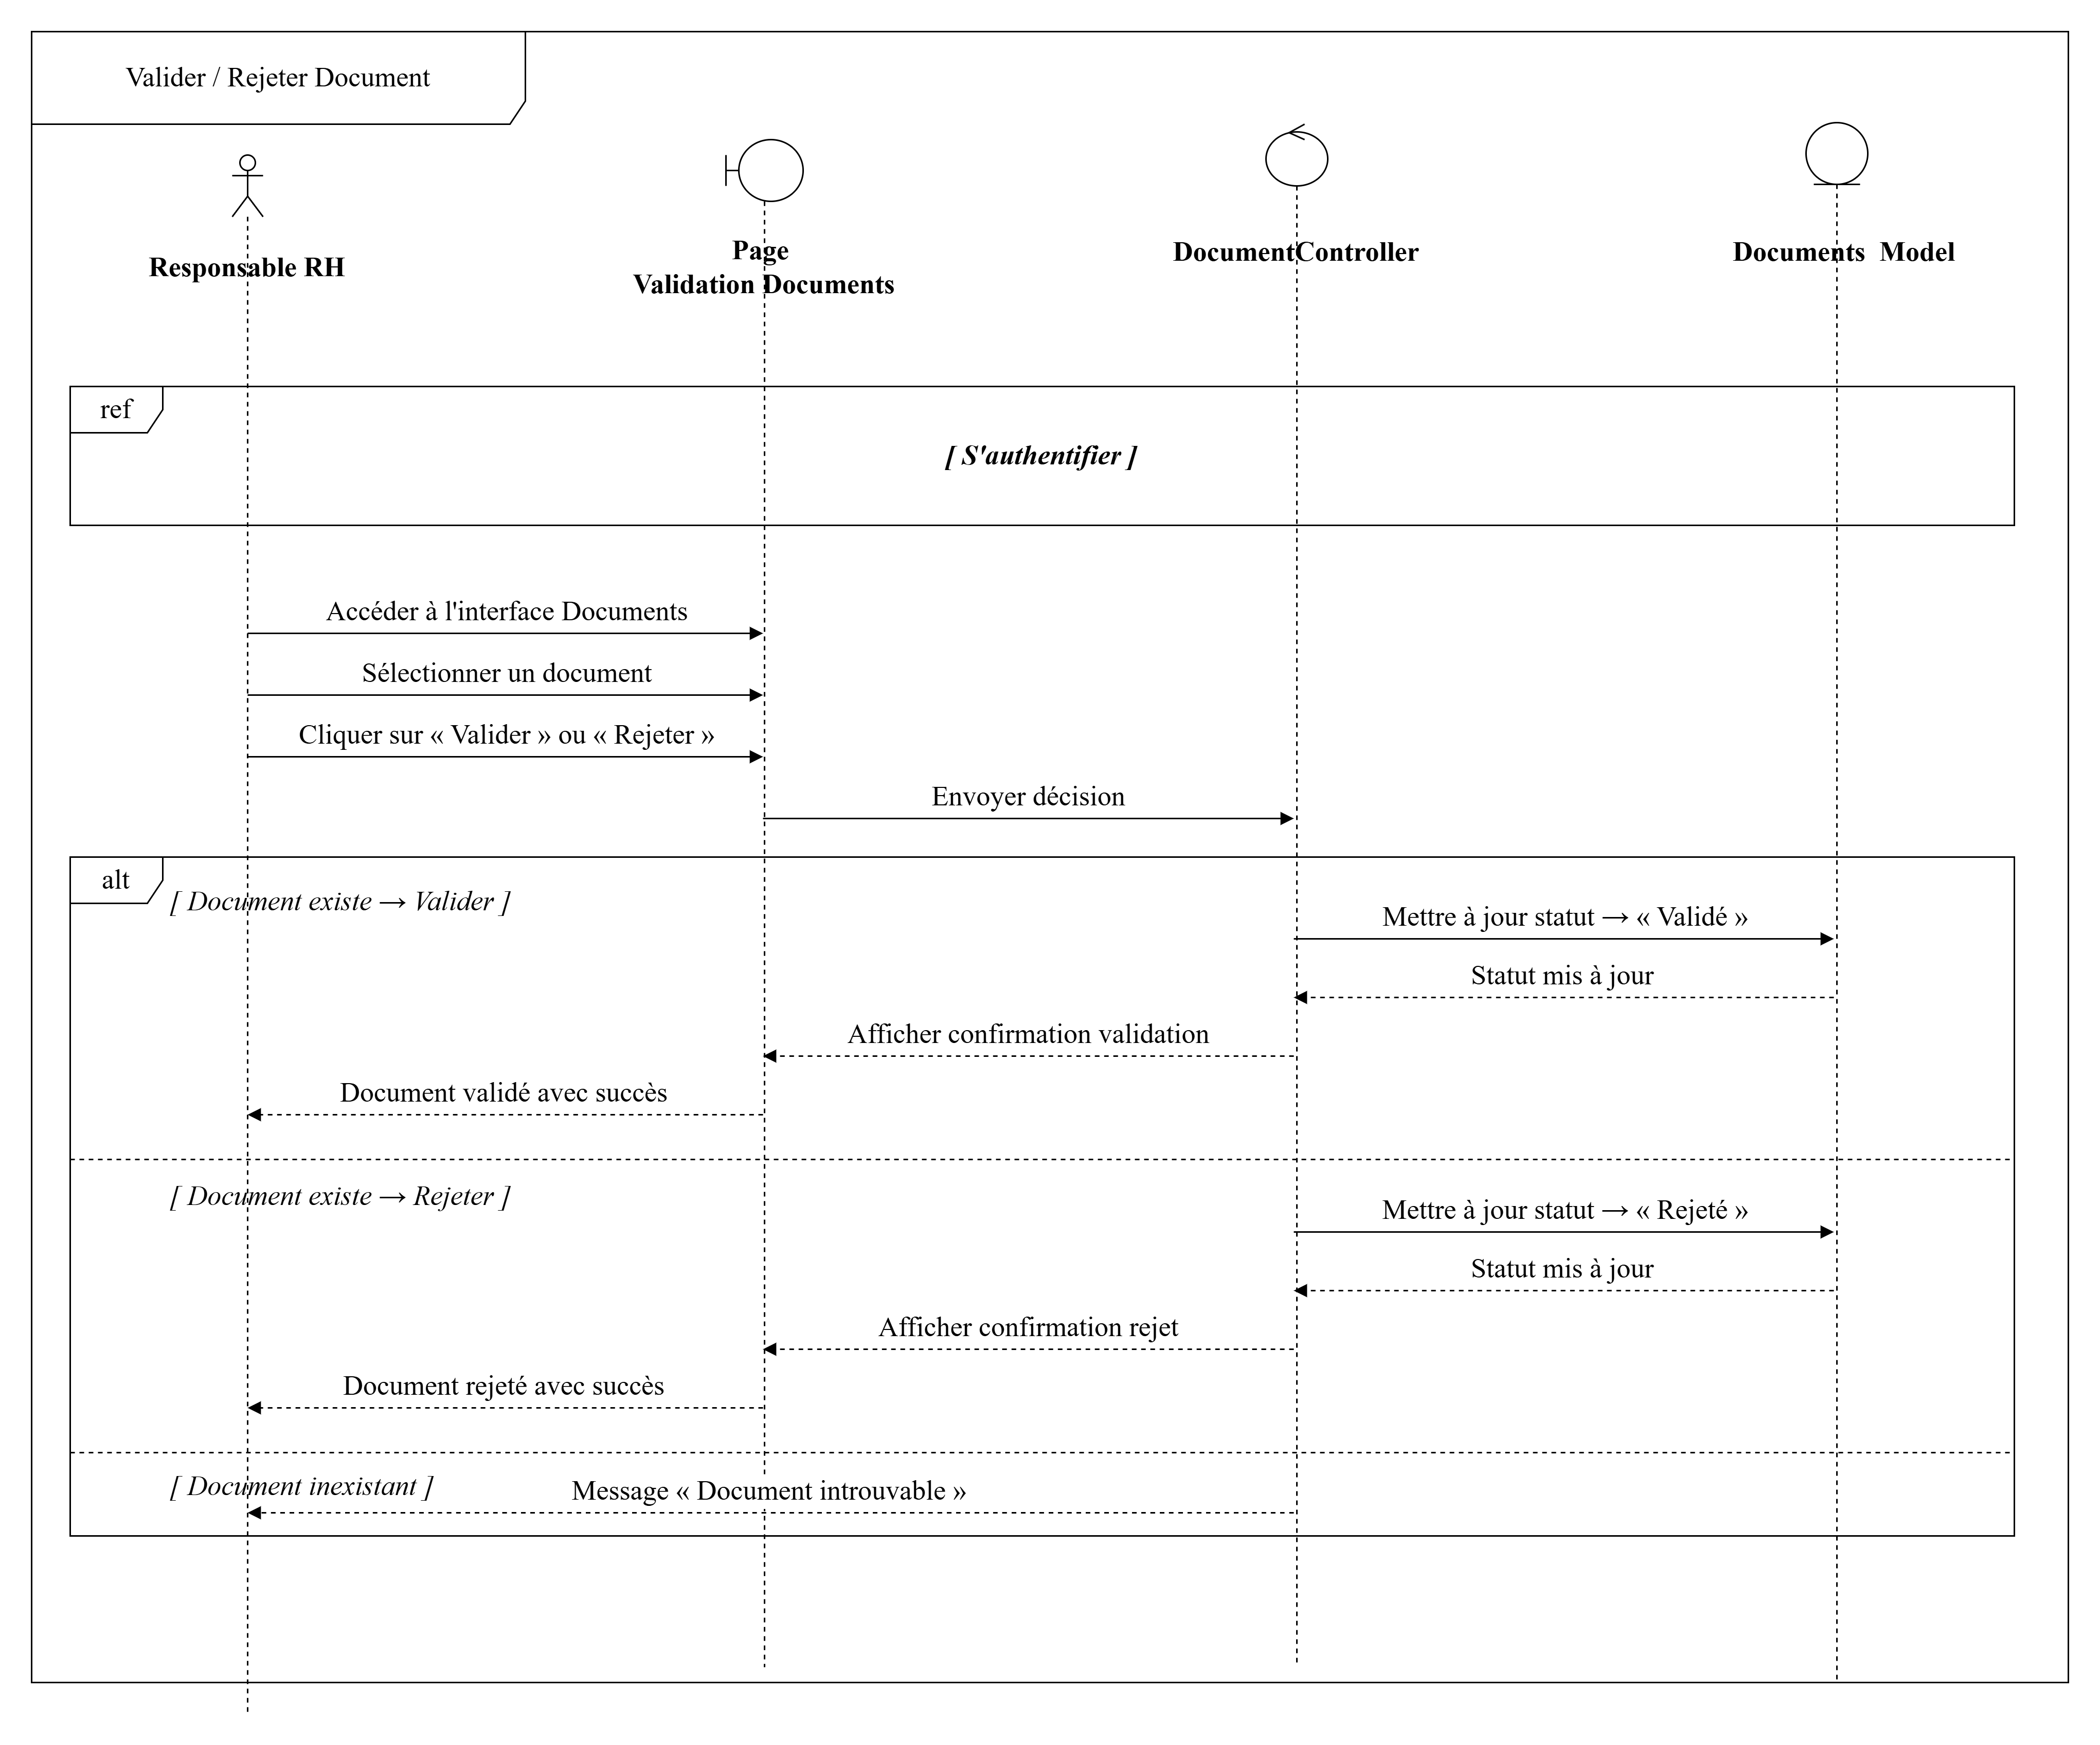
\includegraphics[width=0.9\textwidth]{projet/images/sequence s3/Valider document.drawio.png}
    \caption{Diagramme de séquence du cas d'utilisation «~Valider ou Rejeter document~»}
\end{figure}

\item[$\bullet$] \textbf{Diagramme de séquence du cas d'utilisation «~Consulter prime~»}

Ce diagramme présente la consultation par l'employé de la liste de ses primes attribuées. Il accède à son espace personnel, le système récupère l'historique des primes depuis la base de données et les affiche avec les montants et les dates correspondants.

\begin{figure}[H]
    \centering
    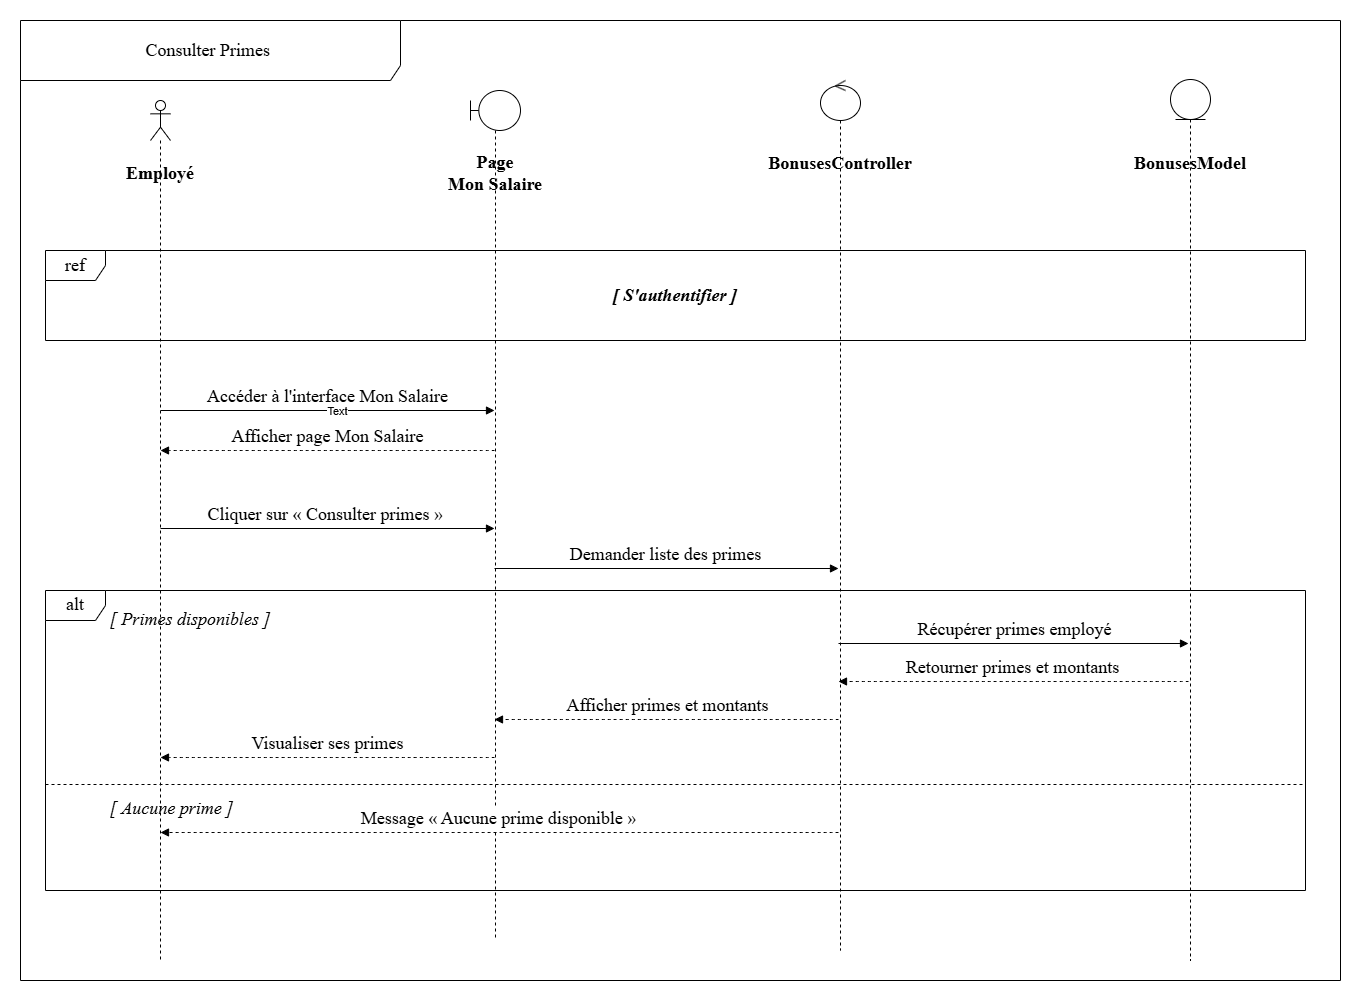
\includegraphics[width=0.9\textwidth]{projet/images/sequence s3/consulter_primes_et_deductions.png}
    \caption{Diagramme de séquence du cas d'utilisation «~Consulter prime~»}
\end{figure}

\item[$\bullet$] \textbf{Diagramme de séquence du cas d'utilisation «~Consulter déduction~»}

Ce diagramme illustre la consultation par l'employé de ses déductions appliquées. Il accède à la section dédiée de son espace personnel, le système récupère les données et les affiche avec les montants et les motifs associés à chaque déduction.

\begin{figure}[H]
    \centering
    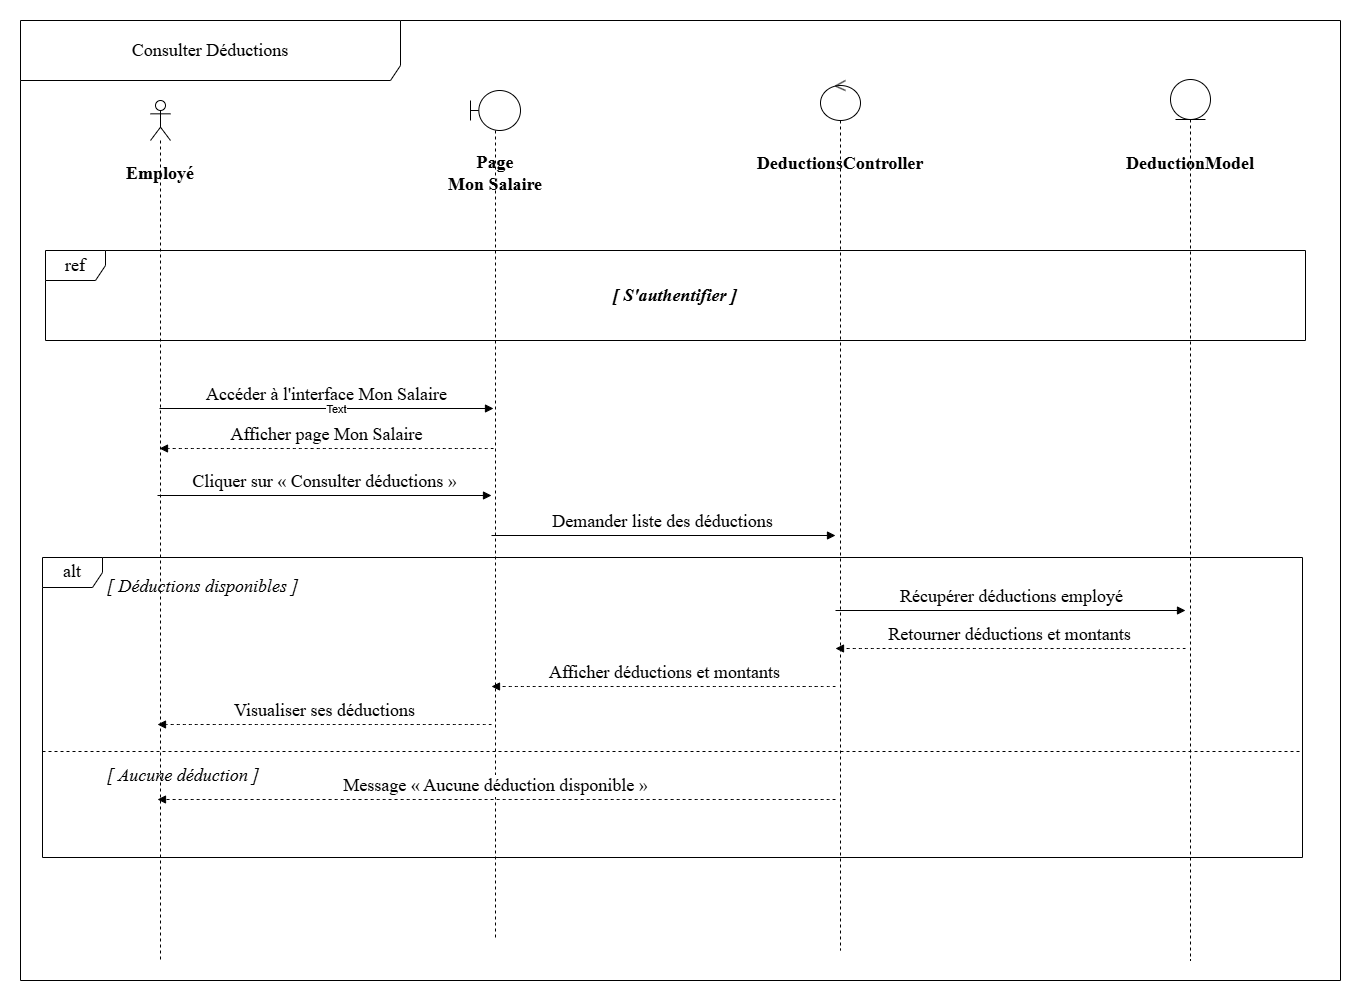
\includegraphics[width=0.9\textwidth]{projet/images/sequence s3/consulter_deductions.png}
    \caption{Diagramme de séquence du cas d'utilisation «~Consulter déduction~»}
\end{figure}

\item[$\bullet$] \textbf{Diagramme de séquence du cas d'utilisation «~Consulter salaire~»}

Ce diagramme décrit la consultation par l'employé du statut de son salaire mensuel. Il accède à son espace personnel, le système interroge la base de données et affiche le statut actuel du salaire, indiquant s'il a été versé ou non.

\begin{figure}[H]
    \centering
    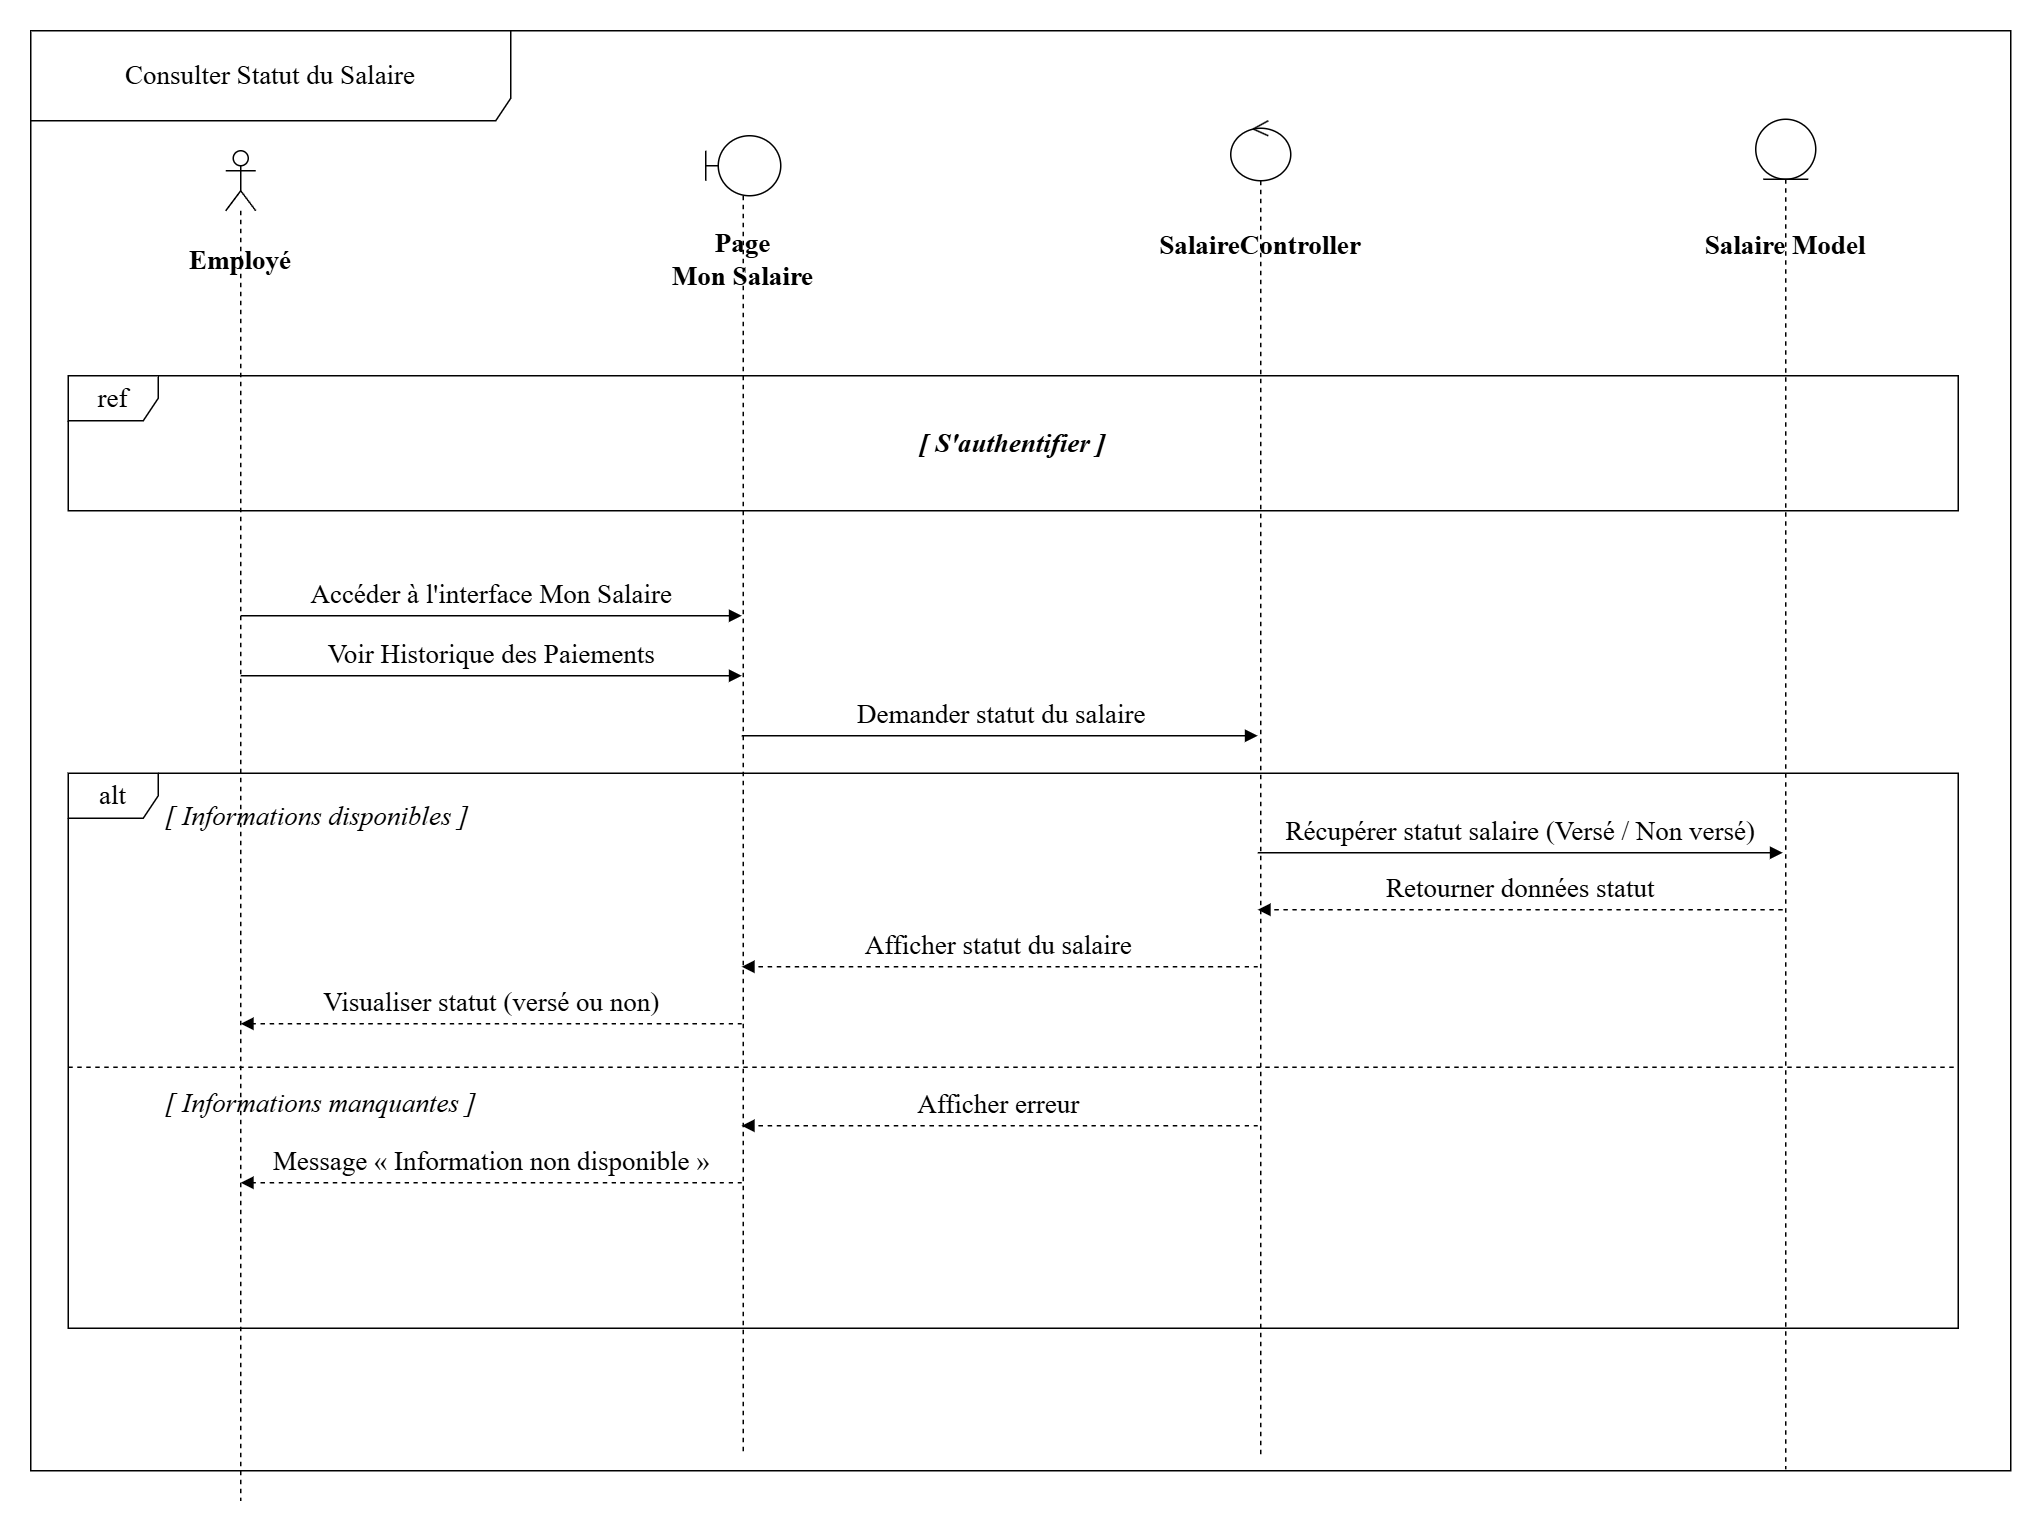
\includegraphics[width=0.9\textwidth]{projet/images/sequence s3/consulter_salaires.png}
    \caption{Diagramme de séquence du cas d'utilisation «~Consulter salaire~»}
\end{figure}

\item[$\bullet$] \textbf{Diagramme de séquence du cas d'utilisation «~Faire une demande de congé~»}

Ce diagramme présente le processus de soumission d'une demande de congé par l'employé. Il saisit les dates de début et de fin ainsi que le motif, le système enregistre la demande et la transmet au Responsable RH pour traitement.

\begin{figure}[H]
    \centering
    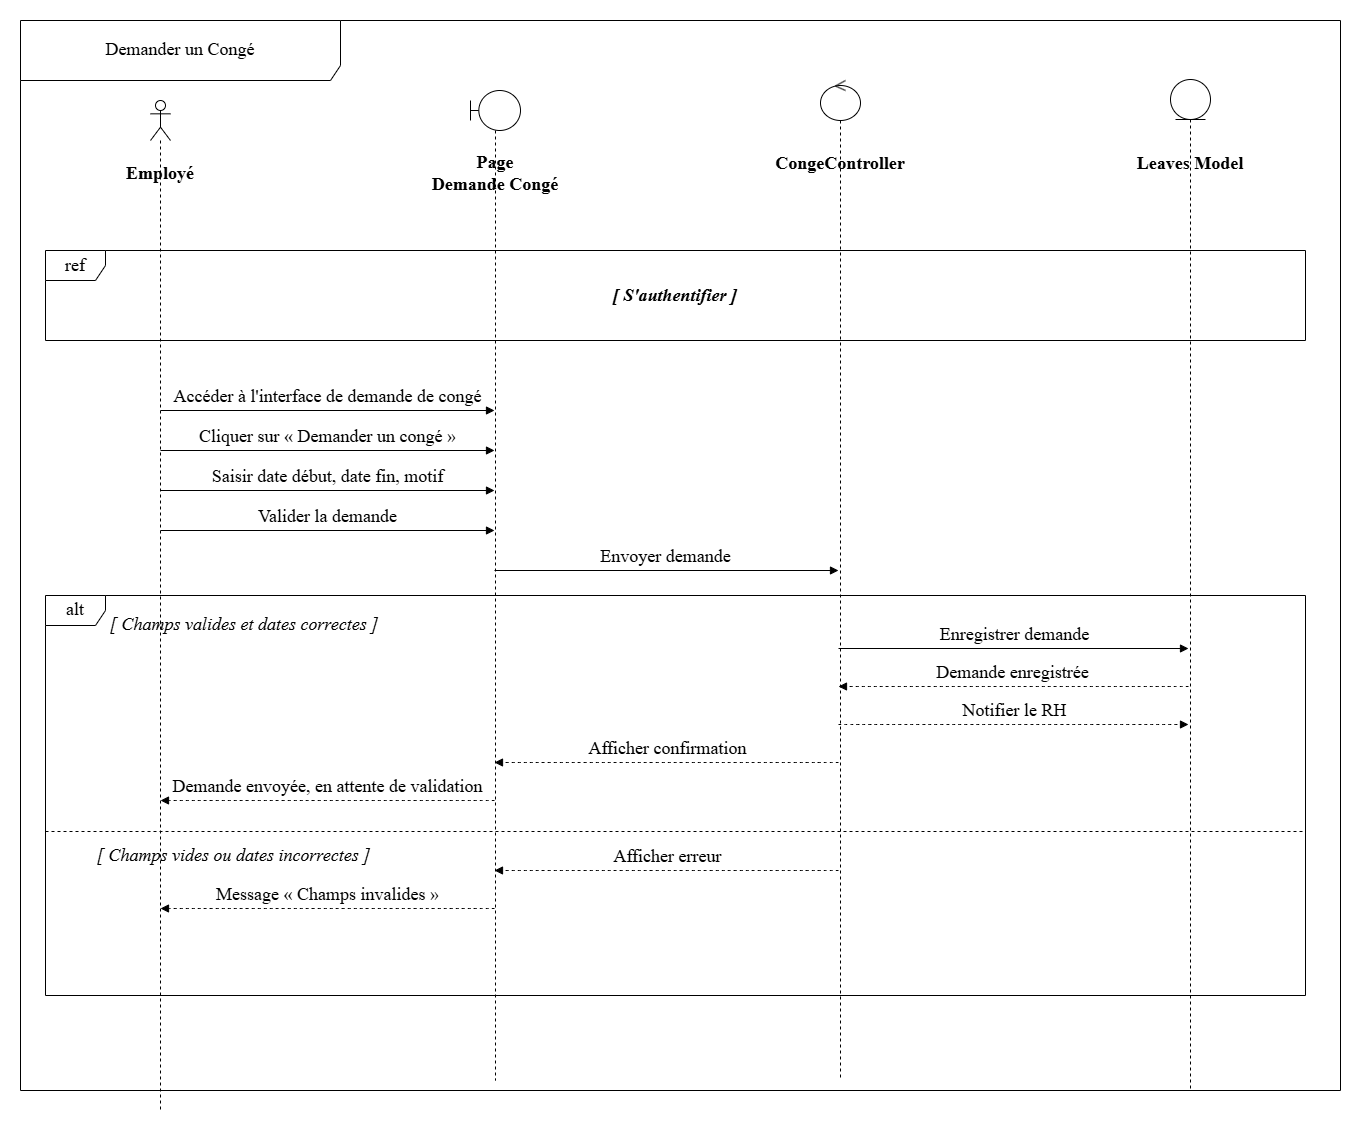
\includegraphics[width=0.9\textwidth]{projet/images/sequence s3/demander conges.drawio.png}
    \caption{Diagramme de séquence du cas d'utilisation «~Faire une demande de congé~»}
\end{figure}

\item[$\bullet$] \textbf{Diagramme de séquence du cas d'utilisation «~Déposer document~»}

Ce diagramme décrit le dépôt d'un document justificatif par l'employé. Il sélectionne le fichier à soumettre, saisit les informations nécessaires et le système enregistre le document avant de notifier le Responsable RH de son arrivée.

\begin{figure}[H]
    \centering
    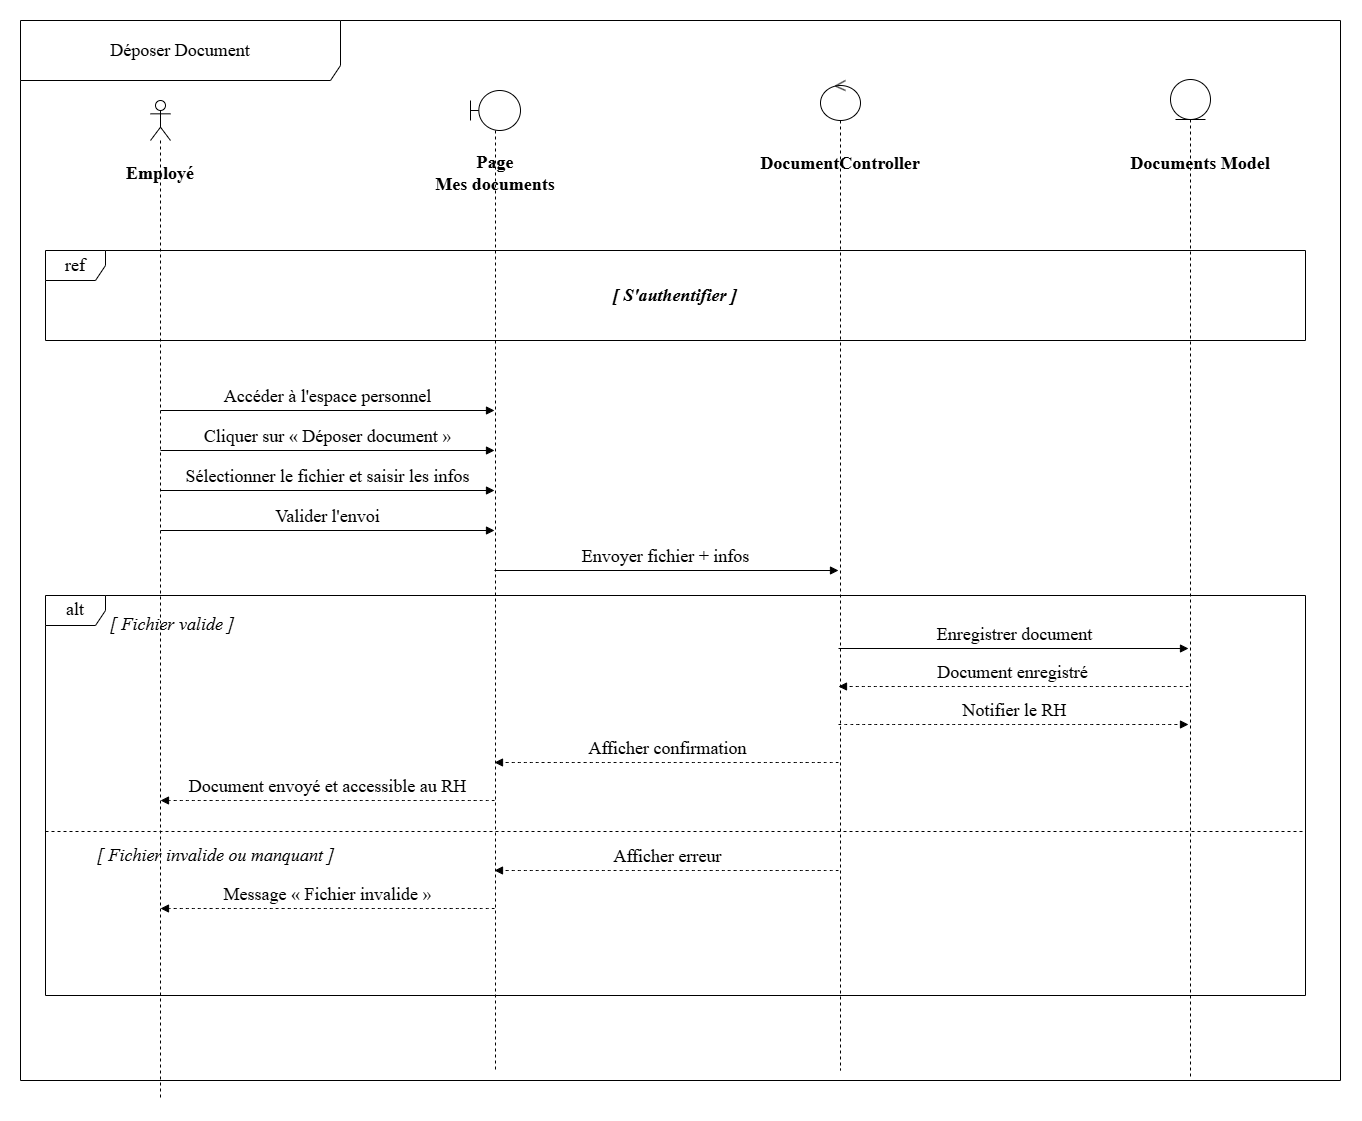
\includegraphics[width=0.9\textwidth]{projet/images/sequence s3/deposer documents.drawio.png}
    \caption{Diagramme de séquence du cas d'utilisation «~Déposer document~»}
\end{figure}

\end{itemize}

\subsubsection{Diagramme de classe de sprint 3}

Le diagramme de classe montre la structure des fonctionnalités de gestion des ressources humaines, notamment les congés, les documents administratifs, les primes, les déductions et les salaires des employés.

\begin{figure}[H]
    \centering
    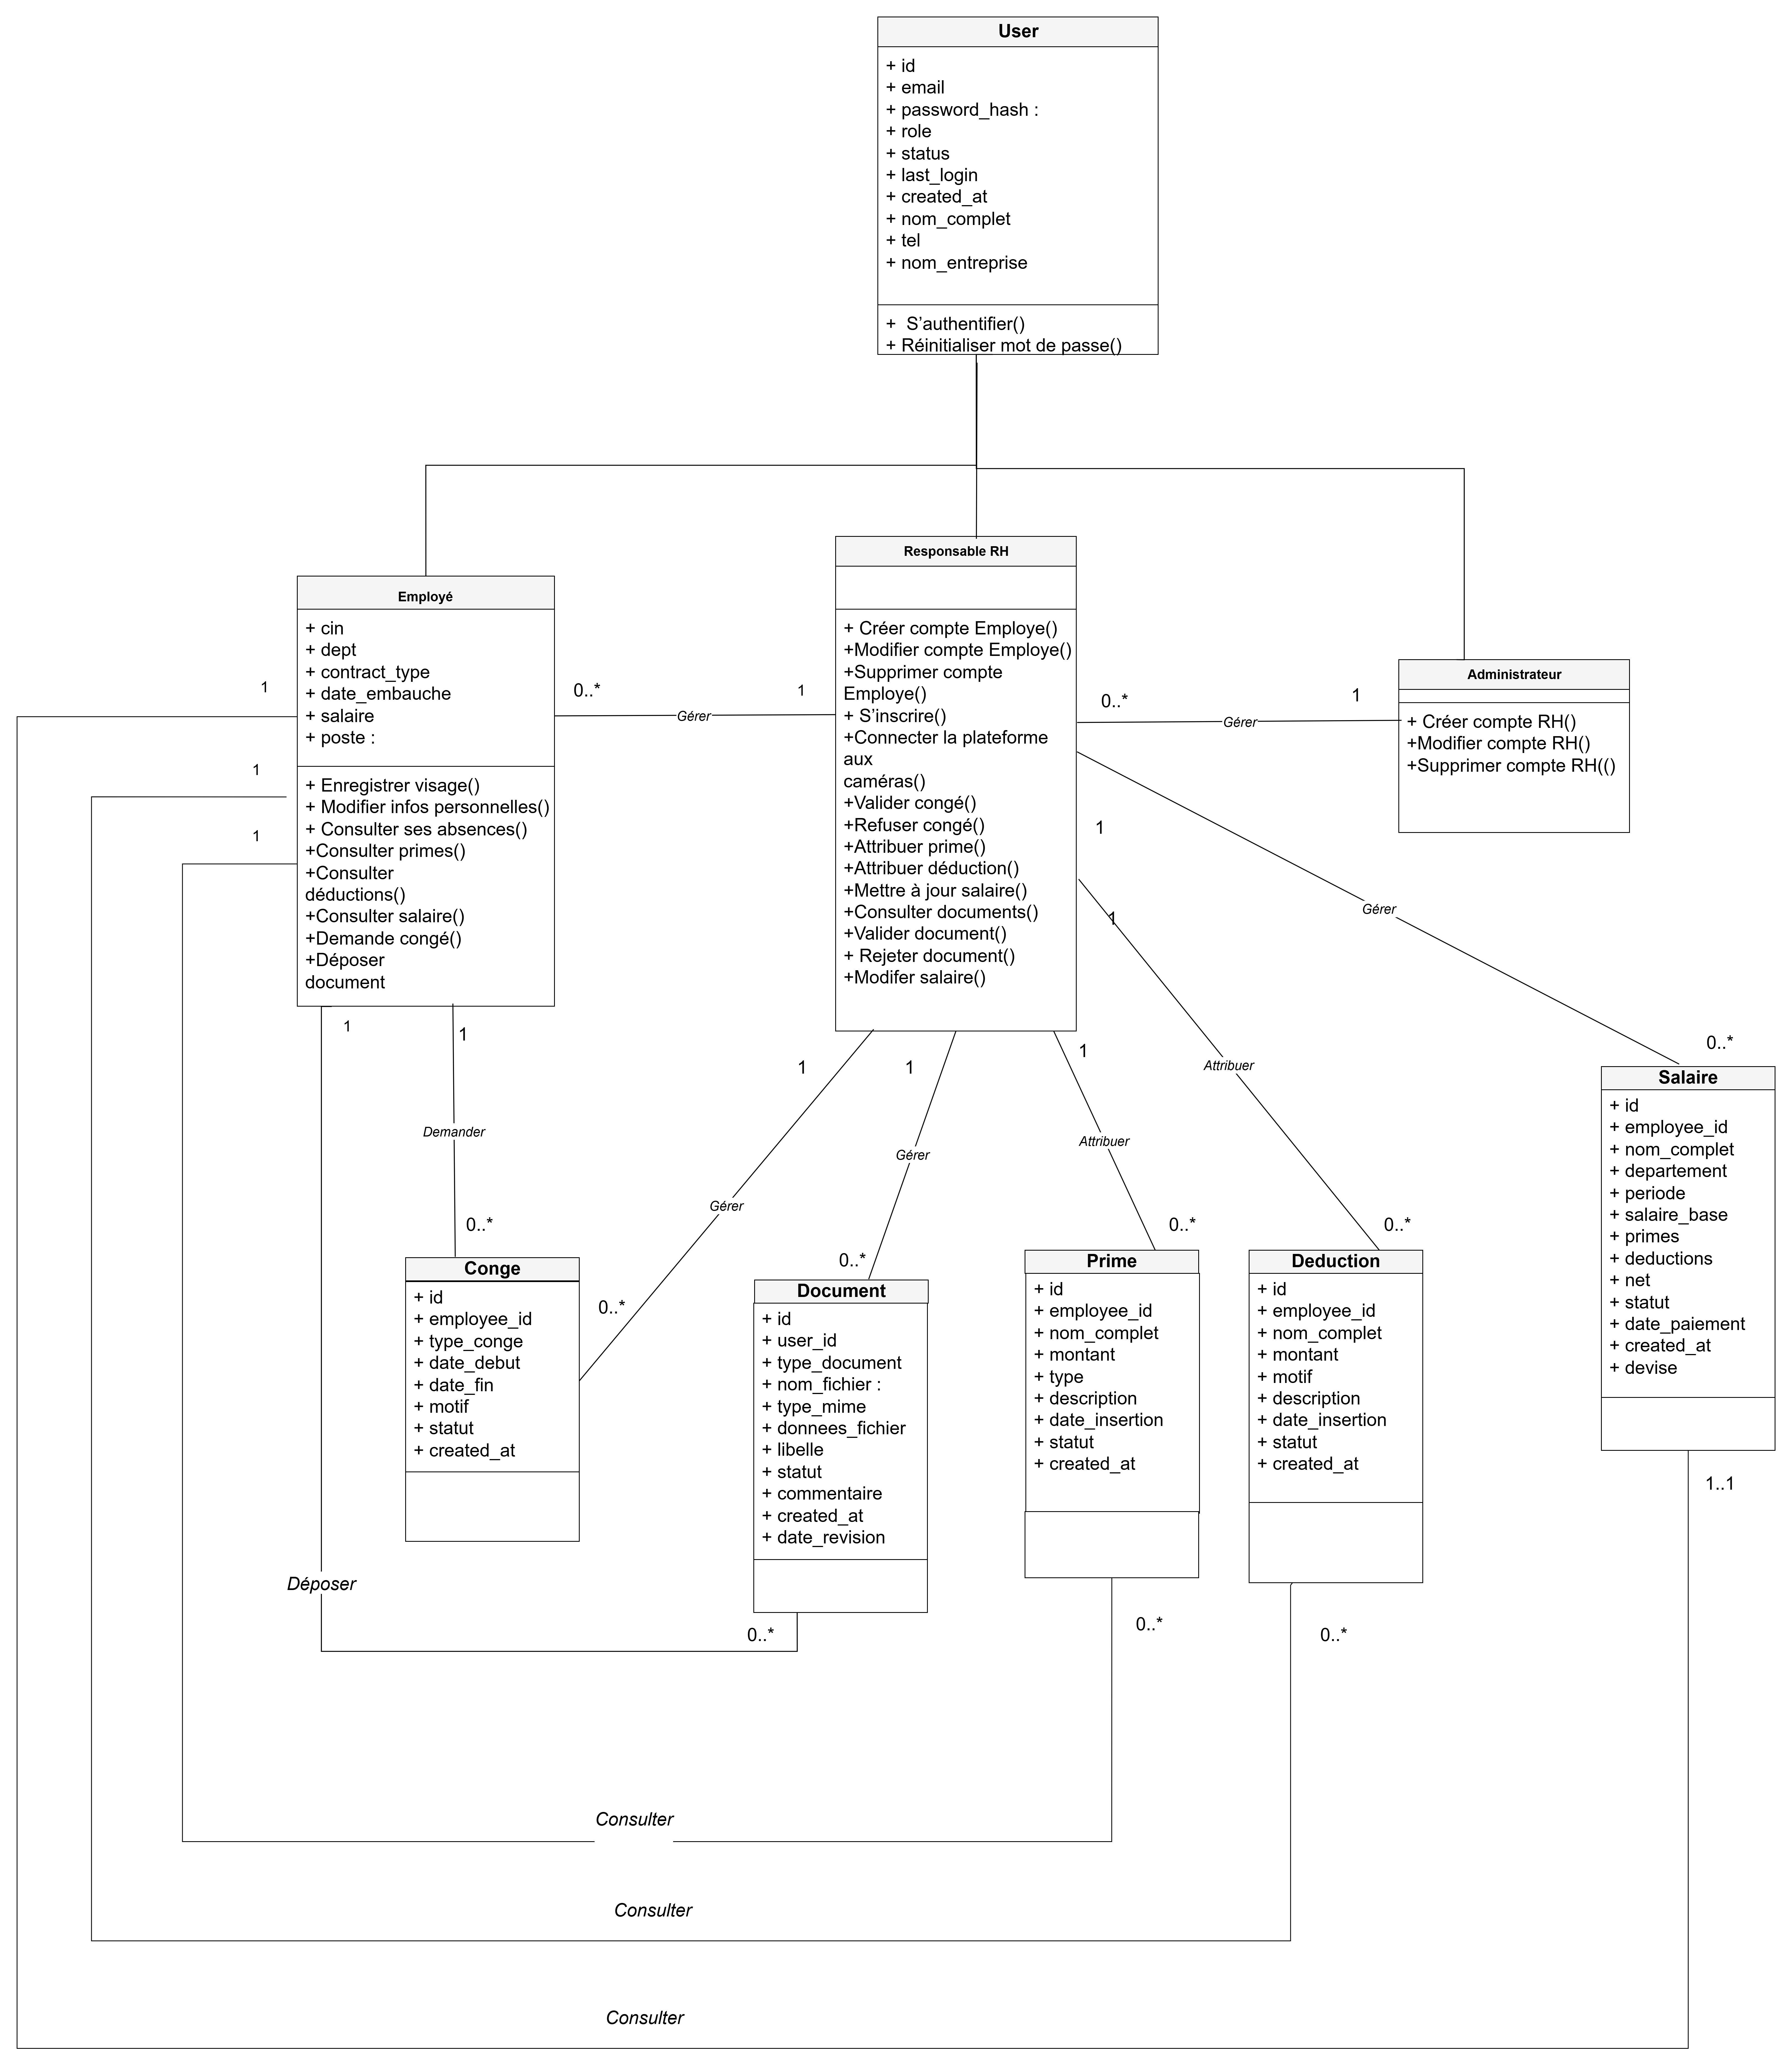
\includegraphics[width=0.9\textwidth]{projet/images/classe finale/s3.png}
    \caption{Diagramme de classe du sprint 3}
    \label{fig:classe_sprint3}
\end{figure}

\subsection{Interfaces réalisées pour le sprint 3}
\begin{itemize}

\item \textbf{Gestion des congés}

Cette interface permet au Responsable RH de consulter les demandes de congé soumises par les employés. Elle offre la possibilité de visualiser les détails de chaque demande, de l’approuver ou de la refuser tout en précisant, si nécessaire, le motif du refus.

\begin{figure}[H]
    \centering
    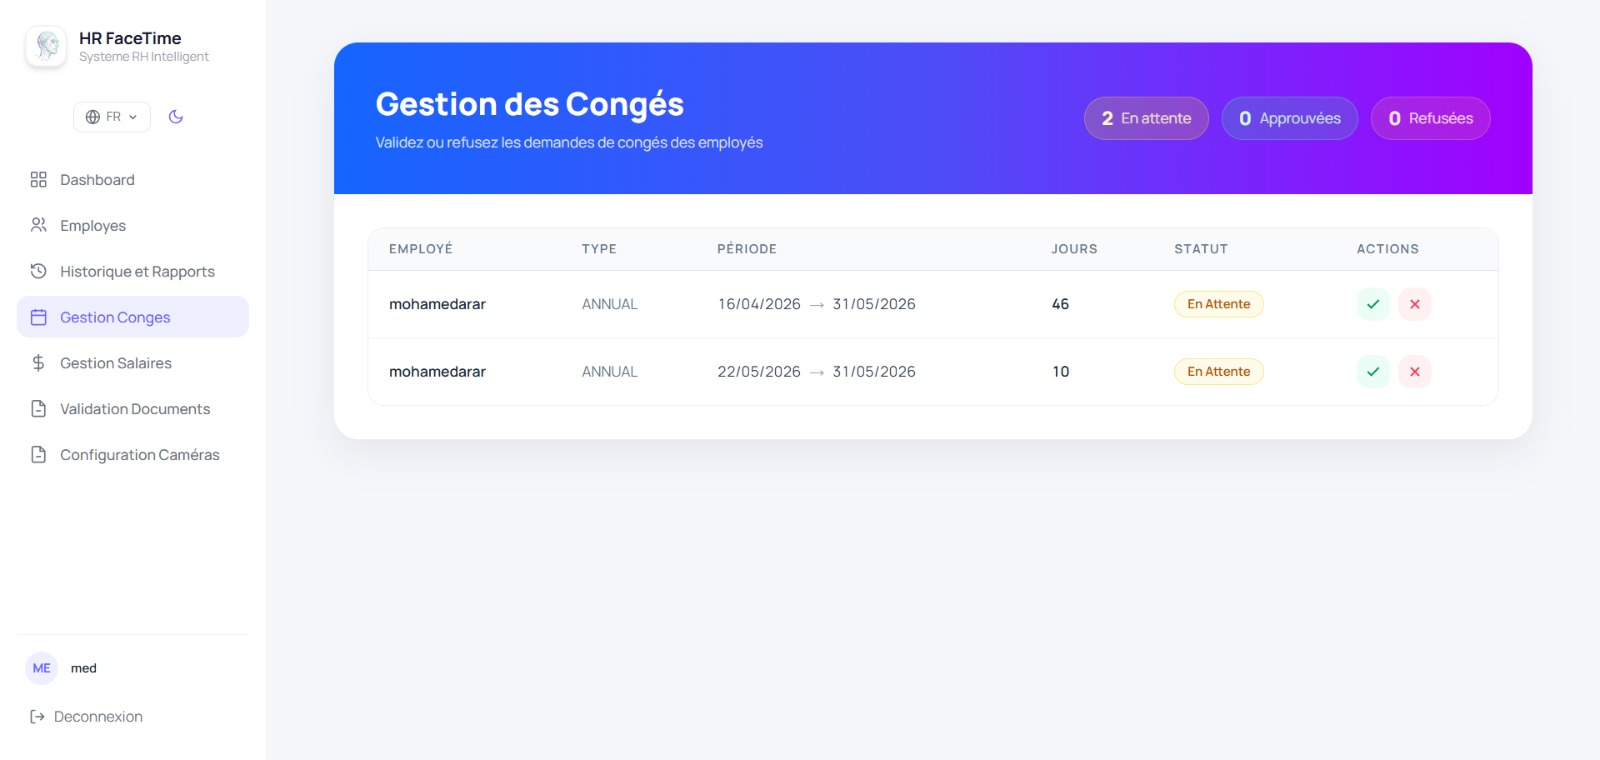
\includegraphics[width=0.9\textwidth]{projet/images/interface/s3/gestion_congee.jpeg}
    \caption{Gestion des congés}
\end{figure}

\item \textbf{Gestion des salaires}
Cette interface permet au Responsable RH de gérer les informations salariales des employés. Elle offre des fonctionnalités de modification du salaire de base, de mise à jour du statut de paiement et de suivi des opérations liées à la paie. Elle permet également l’attribution de primes ainsi que de déductions salariales.

\begin{figure}[H]
    \centering
    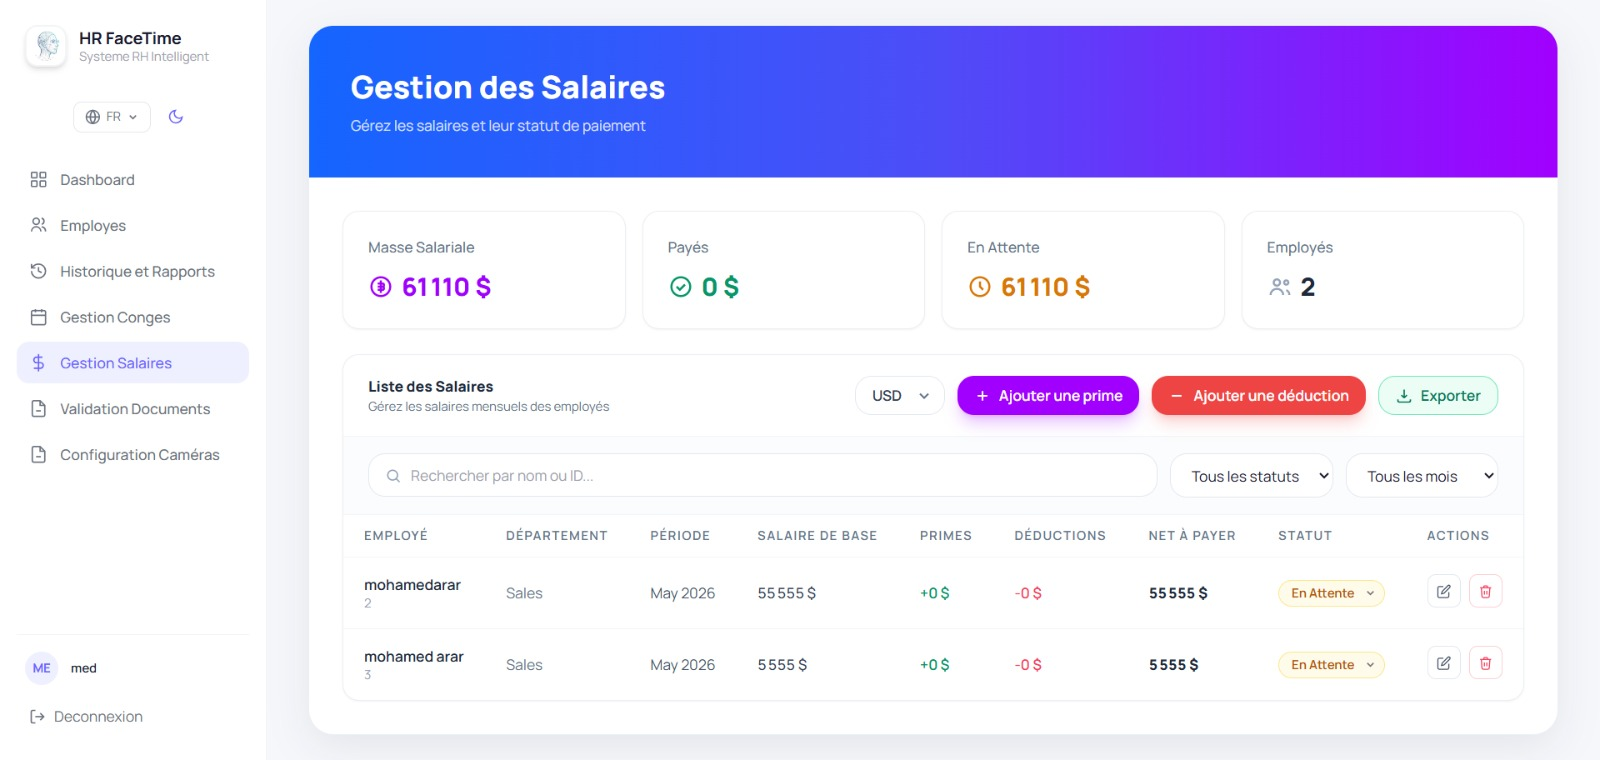
\includegraphics[width=0.9\textwidth]{projet/images/interface/s3/gestion_slaires.jpeg}
    \caption{Gestion des salaires}
\end{figure}



\item \textbf{Gestion des documents administratifs}

Cette interface permet au Responsable RH de consulter les documents déposés par les employés, d’accéder à leurs détails et de les valider ou de les rejeter selon leur conformité.

\begin{figure}[H]
    \centering
    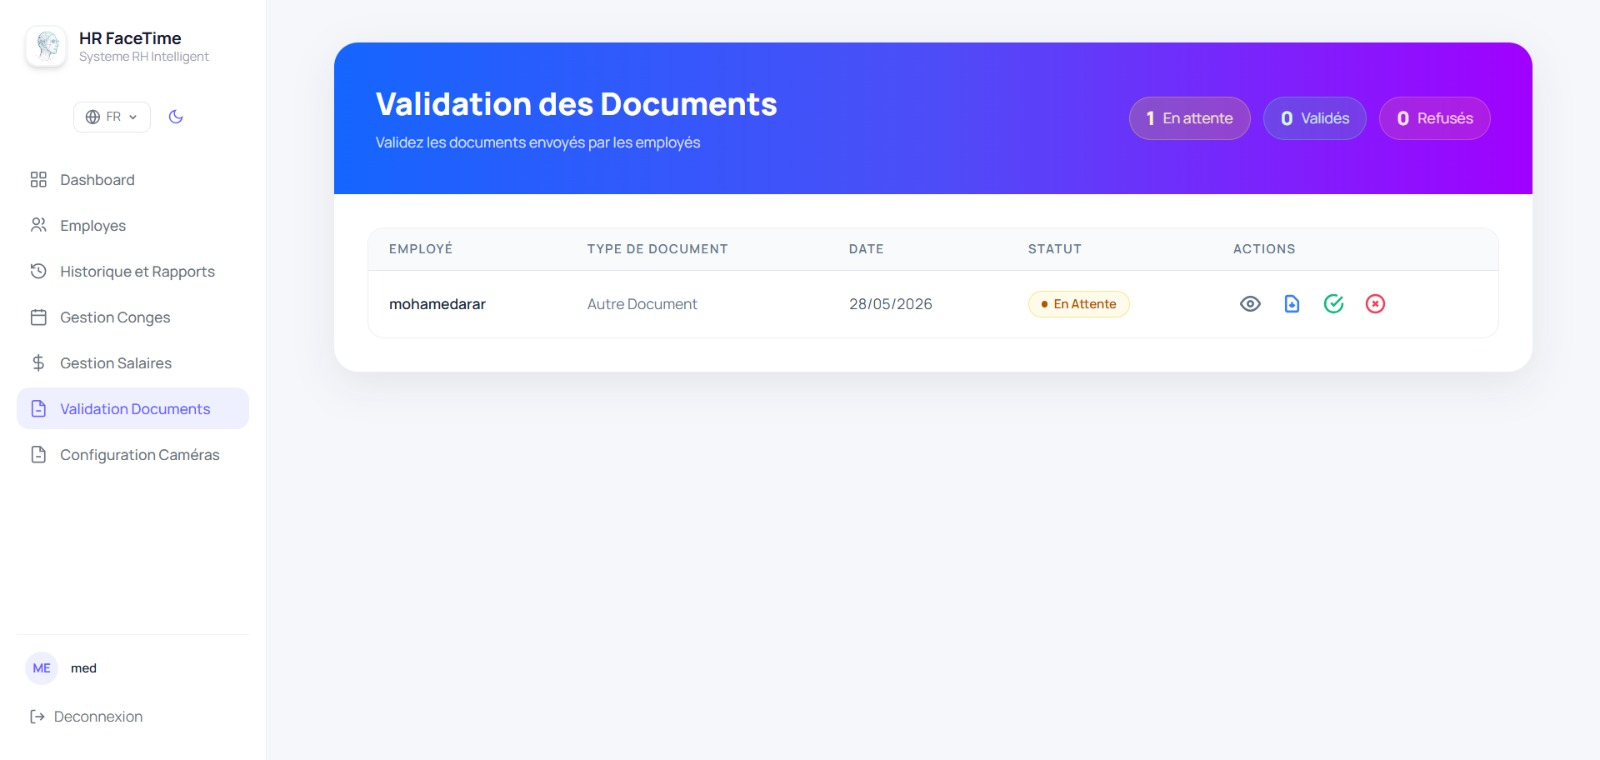
\includegraphics[width=0.9\textwidth]{projet/images/interface/s3/document.jpeg}
    \caption{Gestion des documents administratifs}
\end{figure}

\item \textbf{Mon salaire}

Cette interface permet à l’employé de consulter les informations relatives à sa rémunération, notamment le statut du salaire, les primes et les déductions associées.

\begin{figure}[H]
    \centering
    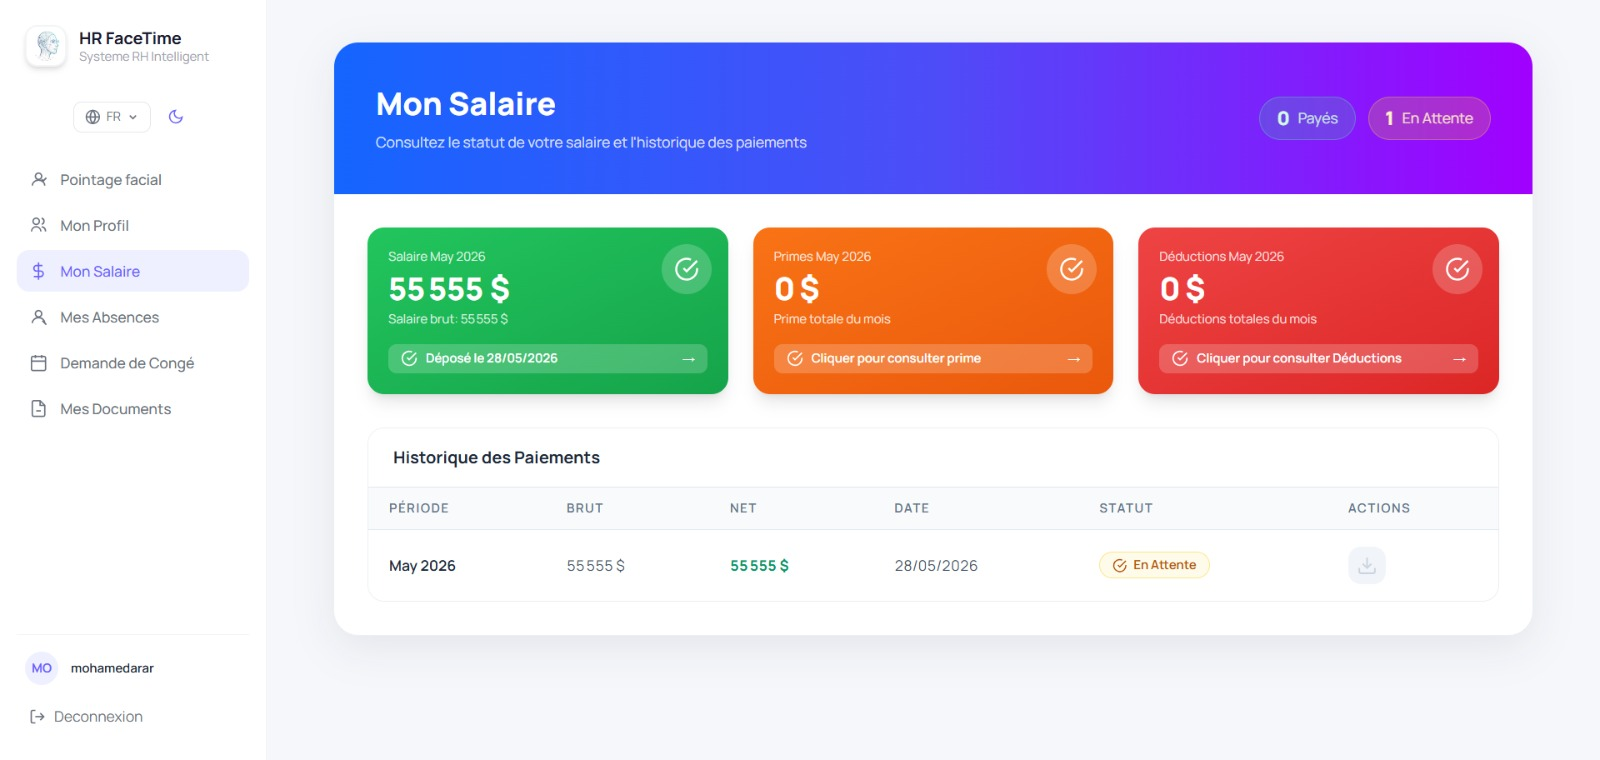
\includegraphics[width=0.9\textwidth]{projet/images/interface/s3/monsalaire.jpeg}
    \caption{Mon salaire}
\end{figure}

\item \textbf{Consultation des primes}

Cette interface permet à l’employé de visualiser l’ensemble des primes qui lui ont été attribuées ainsi que leurs montants et motifs.

\begin{figure}[H]
    \centering
    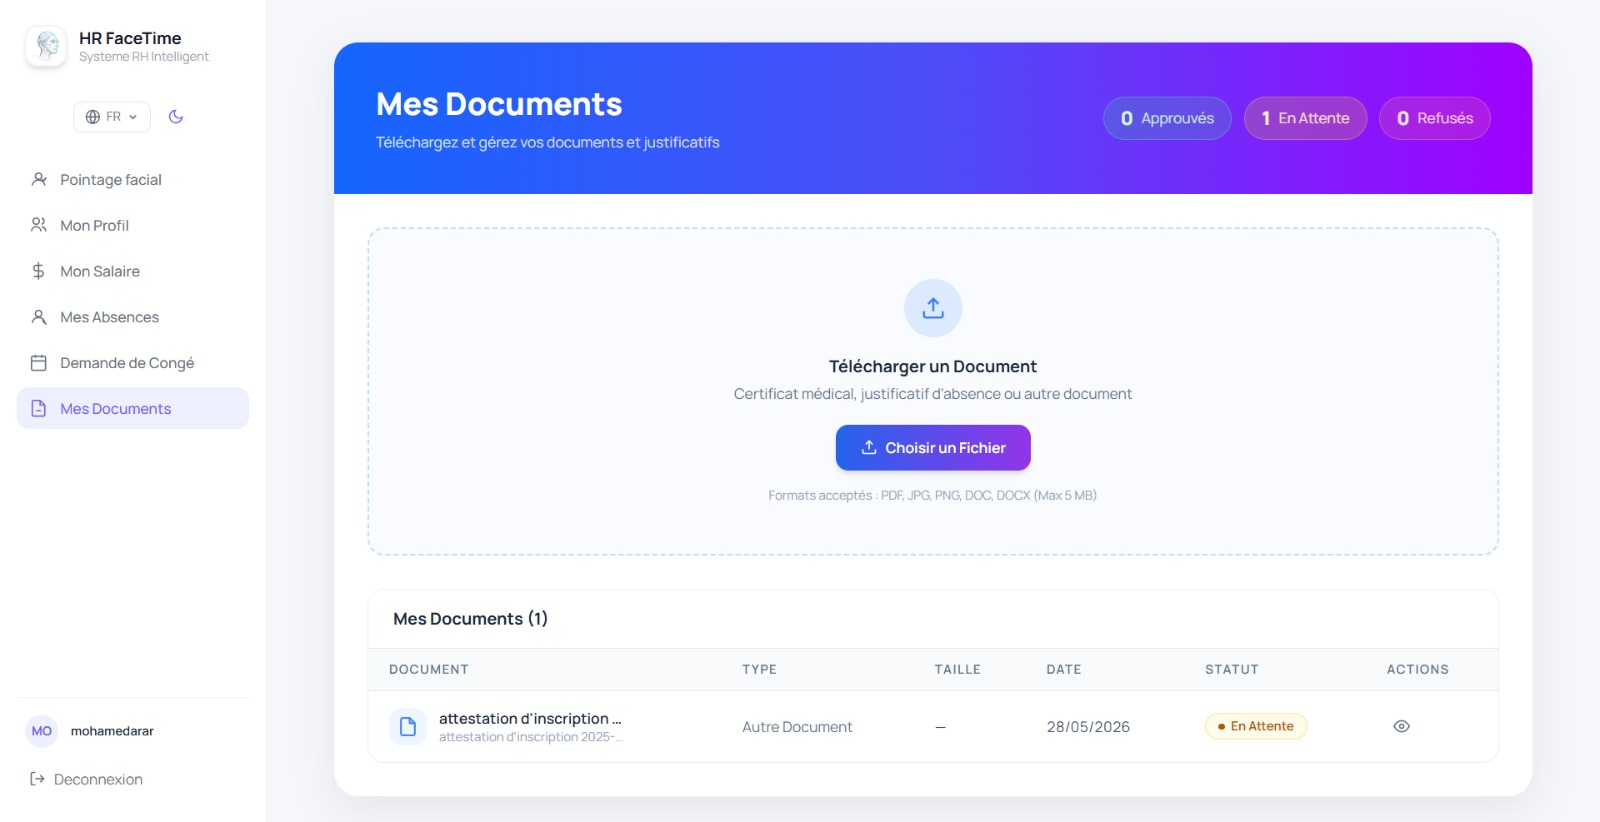
\includegraphics[width=0.9\textwidth]{projet/images/interface/s3/mes_document.jpeg}
    \caption{Consultation des primes}
\end{figure}

\item \textbf{Consultation des déductions}

Cette interface permet à l’employé de consulter les déductions appliquées à son salaire avec les montants et les motifs correspondants.

\begin{figure}[H]
    \centering
    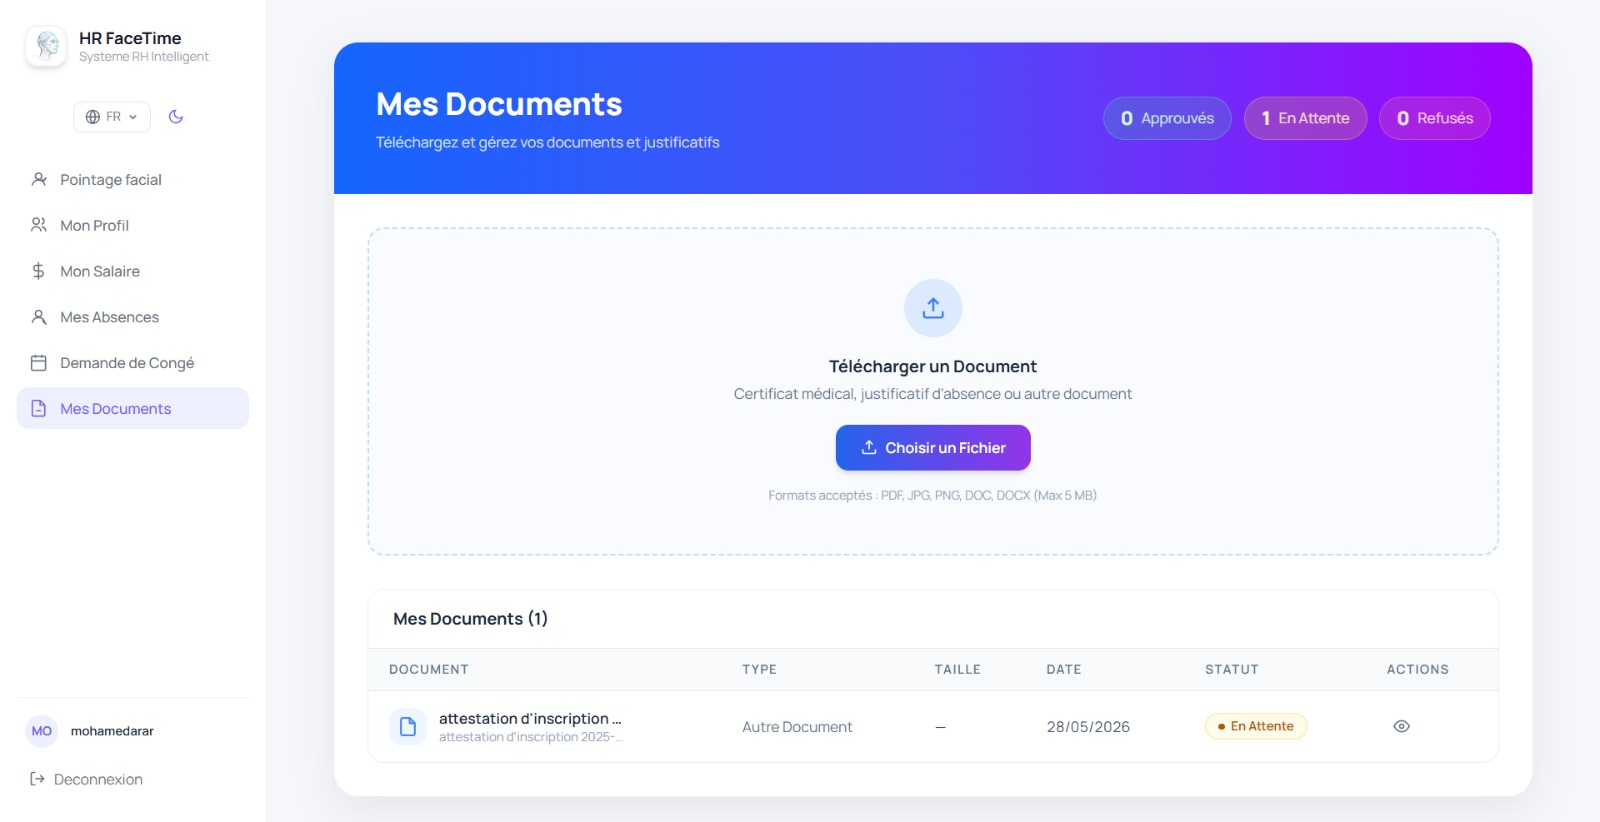
\includegraphics[width=0.9\textwidth]{projet/images/interface/s3/mes_document.jpeg}
    \caption{Consultation des déductions}
\end{figure}

\item \textbf{Demande de congé}

Cette interface permet à l’employé de soumettre une demande de congé en renseignant les dates concernées ainsi que le motif de l’absence.

\begin{figure}[H]
    \centering
    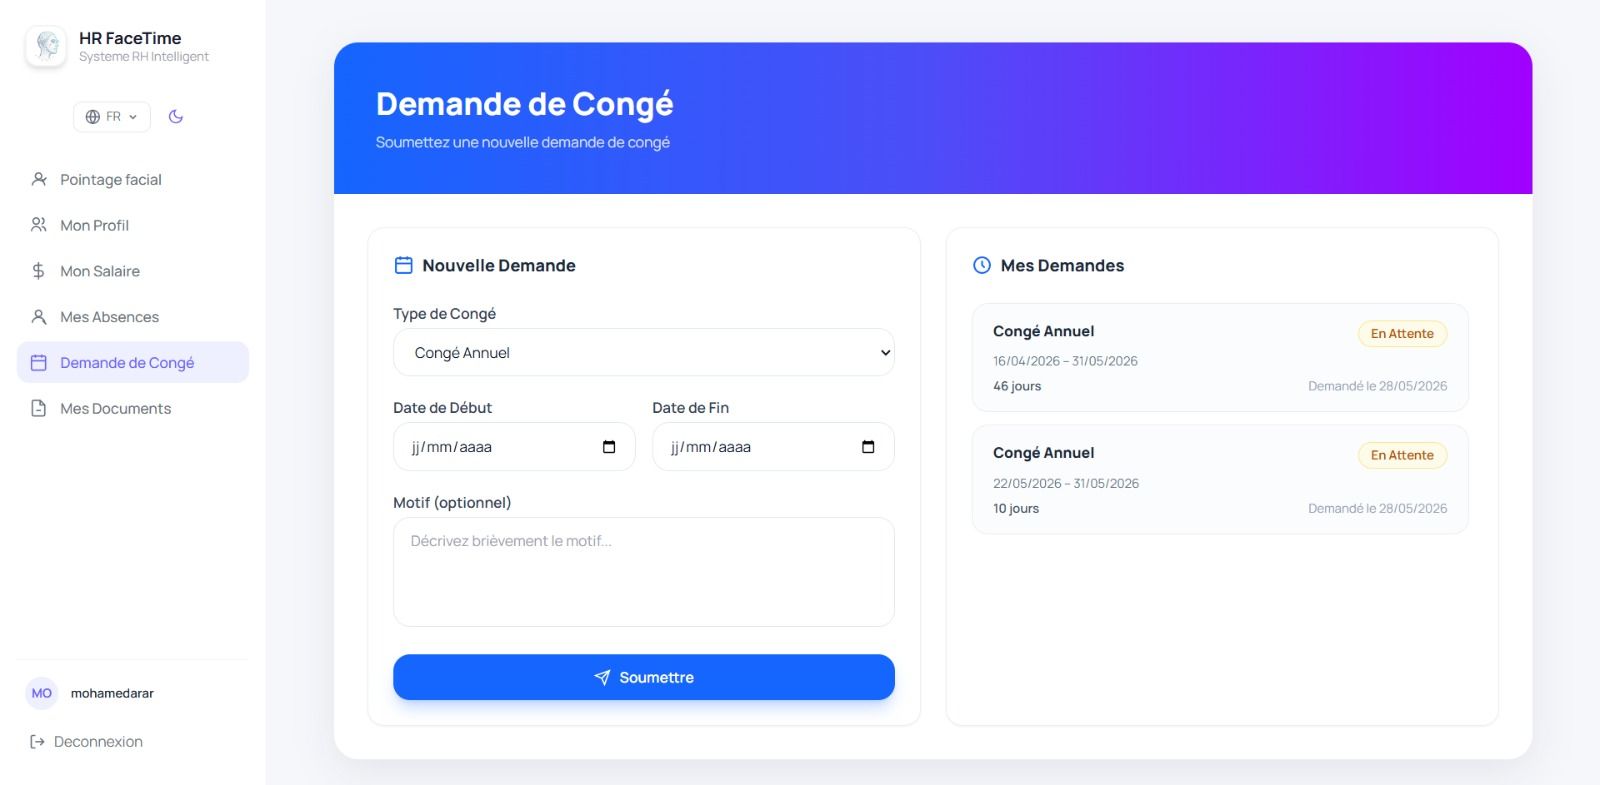
\includegraphics[width=0.9\textwidth]{projet/images/interface/s3/congeé.jpeg}
    \caption{Demande de congé}
\end{figure}

\item \textbf{Dépôt de document}

Cette interface permet à l’employé de déposer des documents administratifs ou justificatifs directement sur la plateforme afin qu’ils soient traités par le Responsable RH.

\begin{figure}[H]
    \centering
    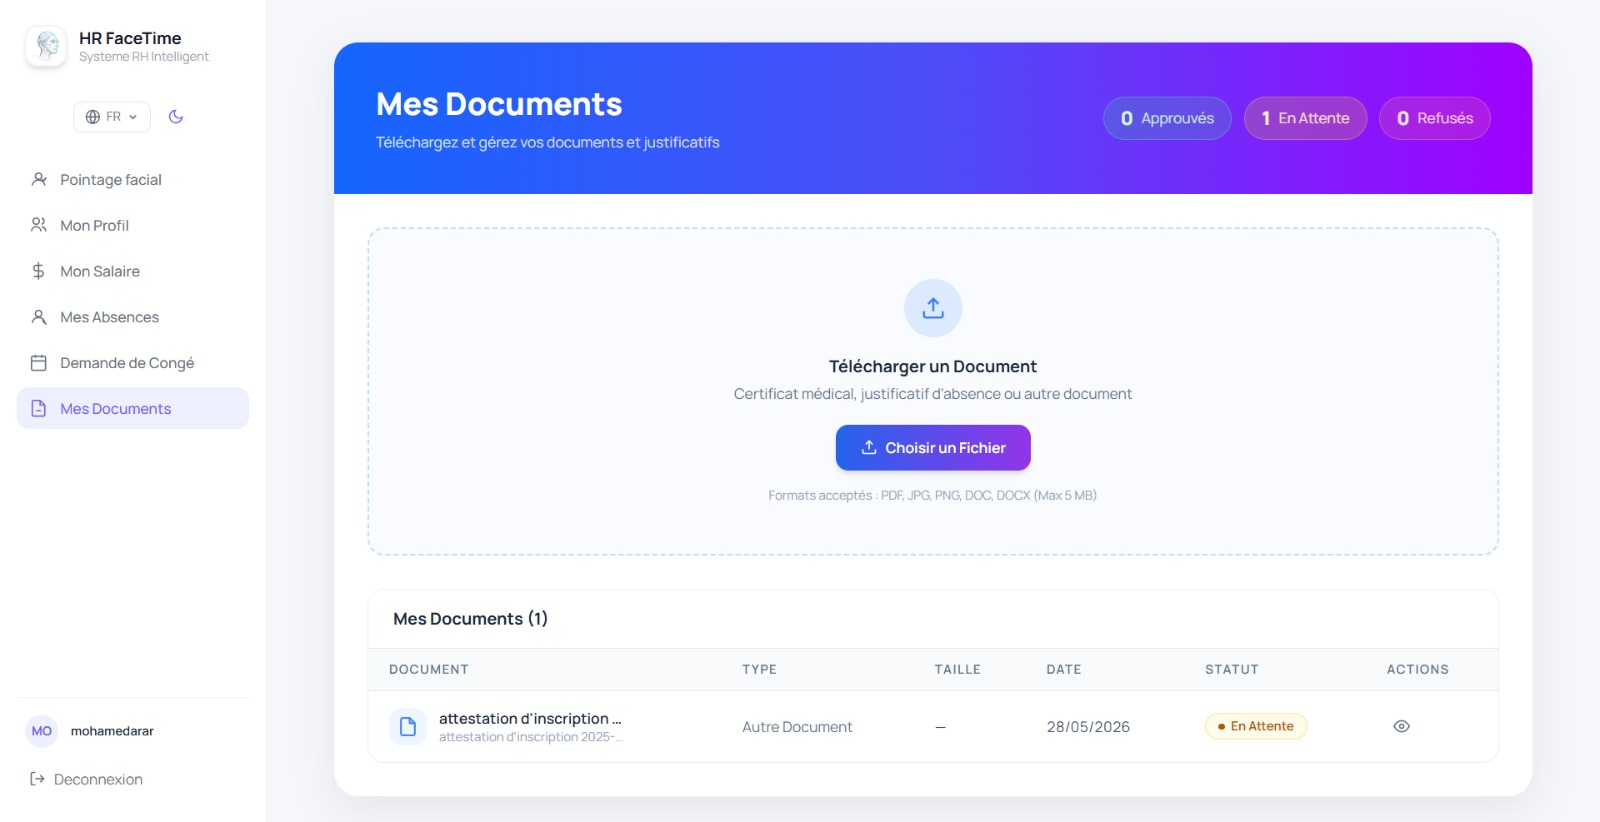
\includegraphics[width=0.9\textwidth]{projet/images/interface/s3/mes_document.jpeg}
    \caption{Dépôt de document}
\end{figure}

\end{itemize}
%==============================================================
\section{Sprint 4: Pilotage RH, Reporting, Paiement et Traçabilité}

Ce sprint a pour objectif de développer les outils de visualisation, paiement de frais permettant un pilotage global du système RH et le suivi des services de la plateforme.

\subsection{Objectif de sprint 4}
L'objectif de ce sprint est l'implémentation des tableaux de bord de l'Administrateur et du Responsable RH, la génération et la mise en export des rapports, ainsi que la gestion de la facturation du service.

\subsection{Durée de sprint 4}
\begin{itemize}
    \item \textbf{Date de début du sprint} : 03/05/2026
    \item \textbf{Date de fin du sprint} : 29/05/2026
\end{itemize}

\subsection{Backlog de sprint 4}
Le sprint backlog relatif à ce sprint est représenté dans le tableau ci-joint.
\begin{longtable}{|>{\centering\arraybackslash}m{0.5cm}|
    >{\centering\arraybackslash}m{3cm}|
    >{\centering\arraybackslash}m{2.5cm}|
    >{\centering\arraybackslash}m{3cm}|
    >{\centering\arraybackslash}m{3cm}|
    >{\centering\arraybackslash}m{0.7cm}|
    >{\centering\arraybackslash}m{0.9cm}|}
\hline
\textbf{ID} & \textbf{User Story} & \textbf{En tant que} & \textbf{Je veux} & \textbf{Afin de} & \textbf{P} & \textbf{C} \\
\hline
4  & Visualiser Dashboard Admin       & Administrateur   & surveiller le système                       & assurer la stabilité          & 5 & 4 \\ \hline
6  & Visualiser Dashboard RH          & Responsable RH   & visualiser les indicateurs RH               & piloter l'activité RH         & 5 & 3 \\ \hline
20 & Générer rapport                 & Responsable RH   & générer des rapports                        & analyser les données RH       & 3 & 3 \\ \hline

21 & Consulter historique             & Responsable RH   & consulter l'historique des actions RH       & assurer la traçabilité        & 4 & 3 \\ \hline


\caption{Backlog Sprint 4 --- Pilotage RH, Reporting \& Gestion des Paiements}
\end{longtable}

\subsection{Spécification fonctionnelle détaillée}

\begin{itemize}

\item \textbf{Diagramme de cas d'utilisation du sprint 4}

\begin{figure}[H]
    \centering
    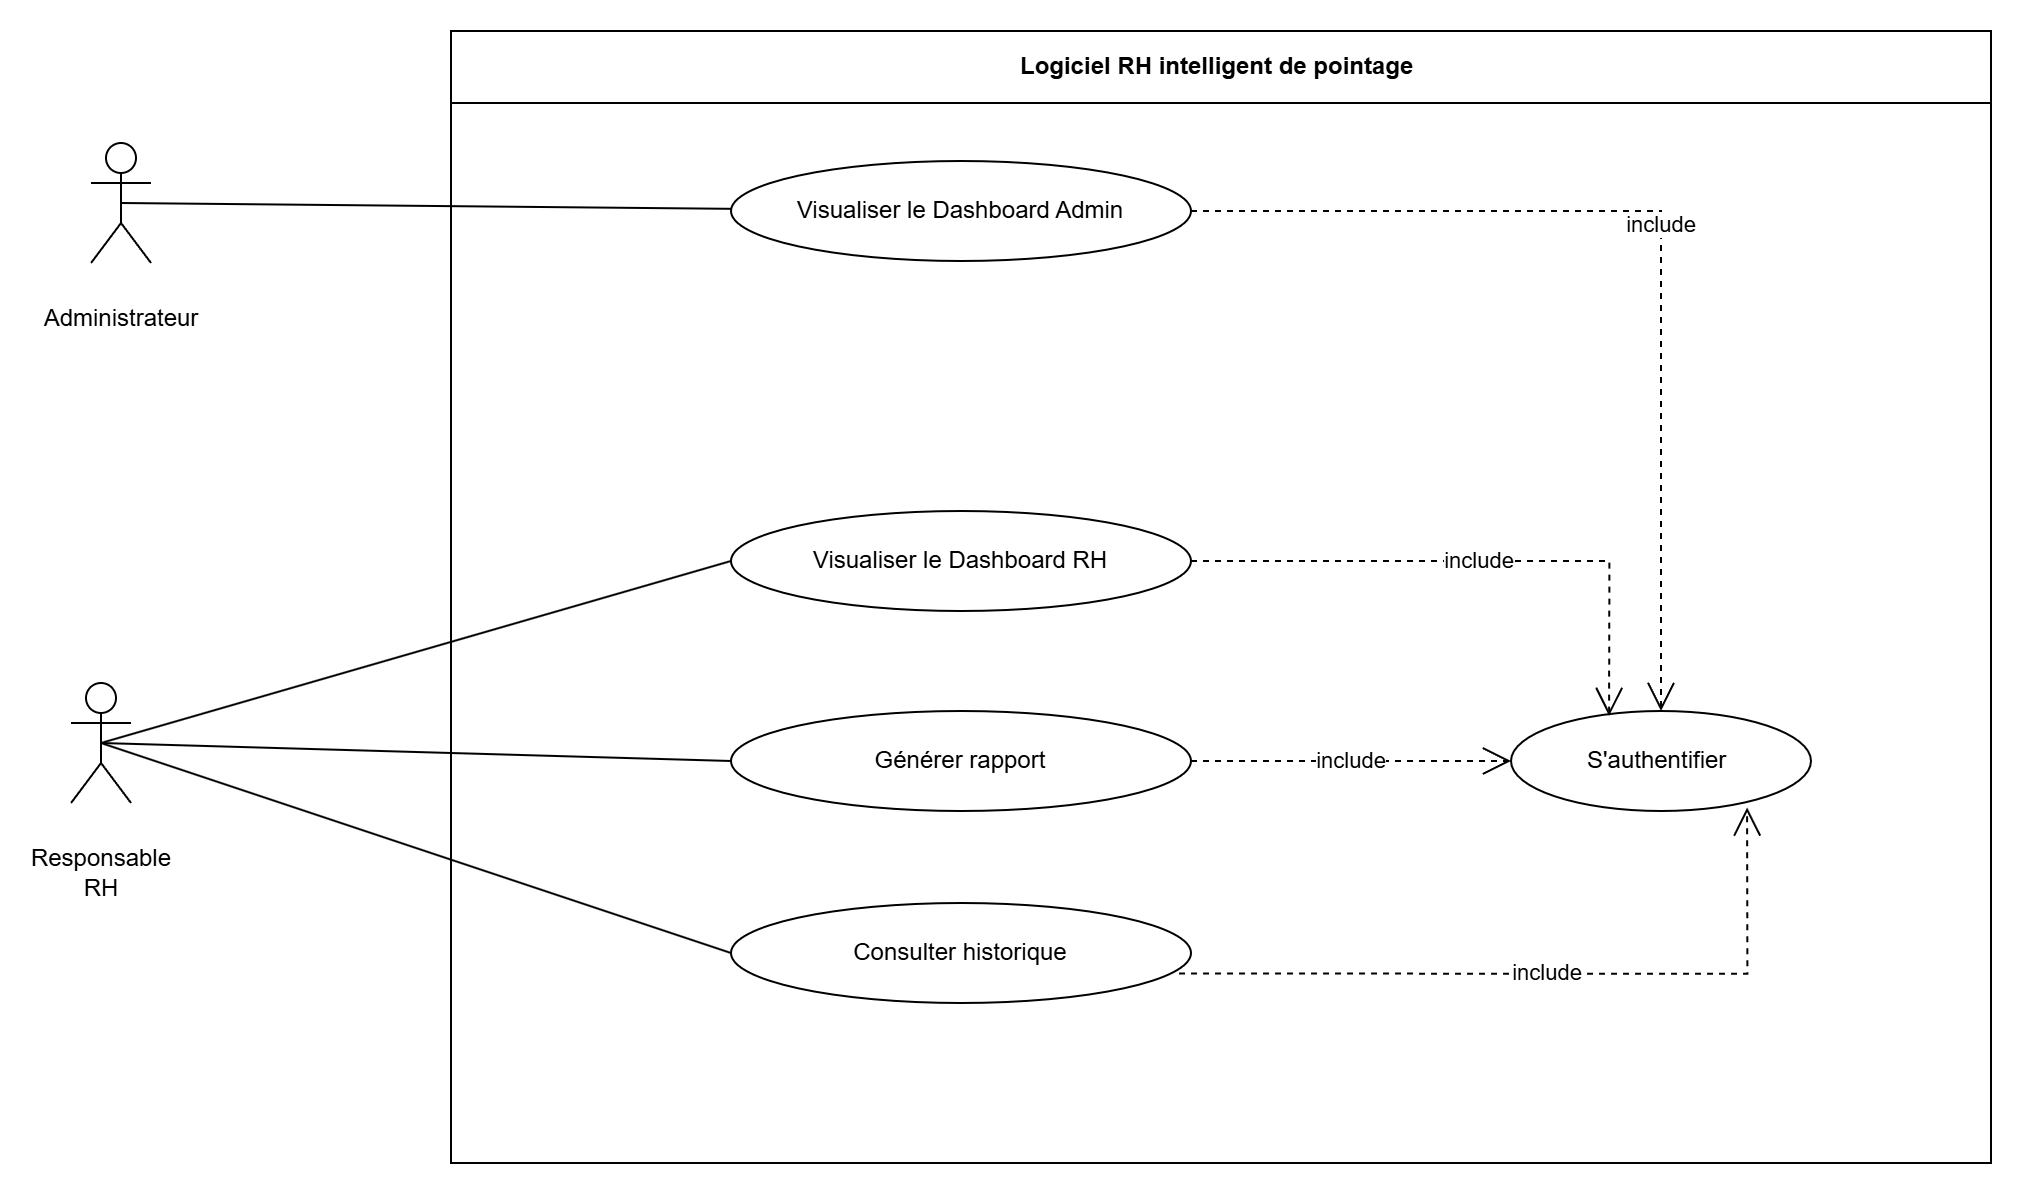
\includegraphics[width=0.9\textwidth]{projet/images/usecase/sprint 4/uses4.drawio.png}
    \caption{Diagramme de Cas d'utilisation du Sprint 4}
    \label{fig:usecase_sprint4}
\end{figure}

\item \textbf{Description textuelle : cas d'utilisation «~Visualiser le Dashboard Administrateur~»}

\begin{center} \begin{longtable}{|p{5cm}|p{11cm}|} \hline \textbf{Nom du cas d'utilisation} & Visualiser tableau de bord administrateur \\ \hline \textbf{Acteurs} & Administrateur \\ \hline \textbf{Objectif} & Permettre à l’administrateur de visualiser le tableau de bord du système \\ \hline \textbf{Préconditions} & L’administrateur est déjà authentifié dans le système \\ \hline \textbf{Scénario nominal} & 1. L’administrateur accède à l’application. \newline 2. Le système détecte une session administrateur active. \newline 3. Le système charge automatiquement les données nécessaires. \newline 4. Le tableau de bord administrateur s’affiche avec les différentes fonctionnalités disponibles. \\ \hline \textbf{Scénario d'exception} & Session inexistante ou expirée $\rightarrow$ redirection vers la page de connexion. \\ \hline \textbf{Post-condition} & Le tableau de bord administrateur est affiché et prêt à être utilisé. \\ \hline \caption{Description textuelle du cas d'utilisation «~Visualiser tableau de bord administrateur~»} \end{longtable} \end{center}


\item \textbf{Description textuelle : cas d'utilisation «~Visualiser le Dashboard RH~»}

\begin{center} \begin{longtable}{|p{5cm}|p{11cm}|} \hline \textbf{Nom du cas d'utilisation} & Visualiser tableau de bord RH \\ \hline \textbf{Acteurs} & Responsable RH \\ \hline \textbf{Objectif} & Permettre au responsable RH de visualiser le tableau de bord des ressources humaines \\ \hline \textbf{Préconditions} & Le responsable RH est déjà authentifié dans le système \\ \hline \textbf{Scénario nominal} & 1. Le responsable RH accède à l’application. \newline 2. Le système détecte une session RH active. \newline 3. Le système charge automatiquement les données et fonctionnalités RH. \newline 4. Le tableau de bord RH s’affiche avec les différentes options disponibles. \\ \hline \textbf{Scénario d'exception} & Session inexistante ou expirée $\rightarrow$ redirection vers la page de connexion. \\ \hline \textbf{Post-condition} & Le tableau de bord RH est affiché et prêt à être utilisé. \\ \hline \caption{Description textuelle du cas d'utilisation «~Visualiser tableau de bord RH~»} \end{longtable} \end{center}



\item \textbf{Description textuelle : cas d'utilisation «~Consulter historique~»}

\begin{center}
\begin{longtable}{|p{5cm}|p{11cm}|}
\hline

\textbf{Nom du cas d'utilisation} & Exporter l'historique \\ \hline

\textbf{Acteurs} & Responsable RH \\ \hline

\textbf{Objectif} & Permettre au responsable RH d’exporter l’historique des absences sous forme de fichier \\ \hline

\textbf{Préconditions} & Responsable RH authentifié et historique déjà consulté \\ \hline

\textbf{Scénario nominal} &
1. Accéder à l’interface de l’historique. \newline
2. Afficher les données sous forme de tableau. \newline
3. Cliquer sur le bouton « Exporter ». \newline
4. Choisir le format (PDF ou Excel). \newline
5. Le système génère le fichier. \newline
6. Téléchargement automatique du fichier. \\ \hline

\textbf{Scénario d'exception} &
Erreur de génération $\rightarrow$ message « Export impossible ». \\ \hline

\textbf{Post-condition} &
Le fichier d’historique est exporté et disponible sur l’appareil. \\ \hline

\caption{Description textuelle du cas d'utilisation «~Exporter l'historique~»}
\end{longtable}
\end{center}

\item \textbf{Description textuelle : cas d'utilisation «~Exporter rapport~»}

\begin{center}
\begin{longtable}{|p{5cm}|p{11cm}|}
\hline

\textbf{Nom du cas d'utilisation} & Exporter rapport \\ \hline

\textbf{Acteurs} & Responsable RH \\ \hline

\textbf{Objectif} & Générer et exporter un rapport RH \\ \hline

\textbf{Préconditions} & Responsable RH authentifié \\ \hline

\textbf{Scénario nominal} &
1. Accéder à l’interface principale. \newline
2. Cliquer sur le menu « Historique ». \newline
3. Accéder à la section « Rapports et Analytics ». \newline
4. Sélectionner le type de rapport et la période souhaitée. \newline
5. Cliquer sur le bouton « Exporter ». \newline
6. Le système génère automatiquement le rapport. \newline
7. Le fichier est téléchargé pour consultation. \\ \hline

\textbf{Scénario d'exception} &
Erreur lors de la génération ou de l’exportation $\rightarrow$ message « Export impossible ». \\ \hline

\textbf{Post-condition} &
Le rapport est généré et disponible pour consultation ou téléchargement. \\ \hline

\caption{Description textuelle du cas d'utilisation «~Exporter rapport~»}
\end{longtable}
\end{center}



\end{itemize}

\subsection{Conception}
\subsubsection{Diagrammes de séquence}

\begin{itemize}

\item[$\bullet$] \textbf{Diagramme de séquence du cas d'utilisation «~Visualiser le Dashboard (Administrateur)~»}



% NOTE: image manquante dans le source original — à compléter
\begin{figure}[H]
    \centering
    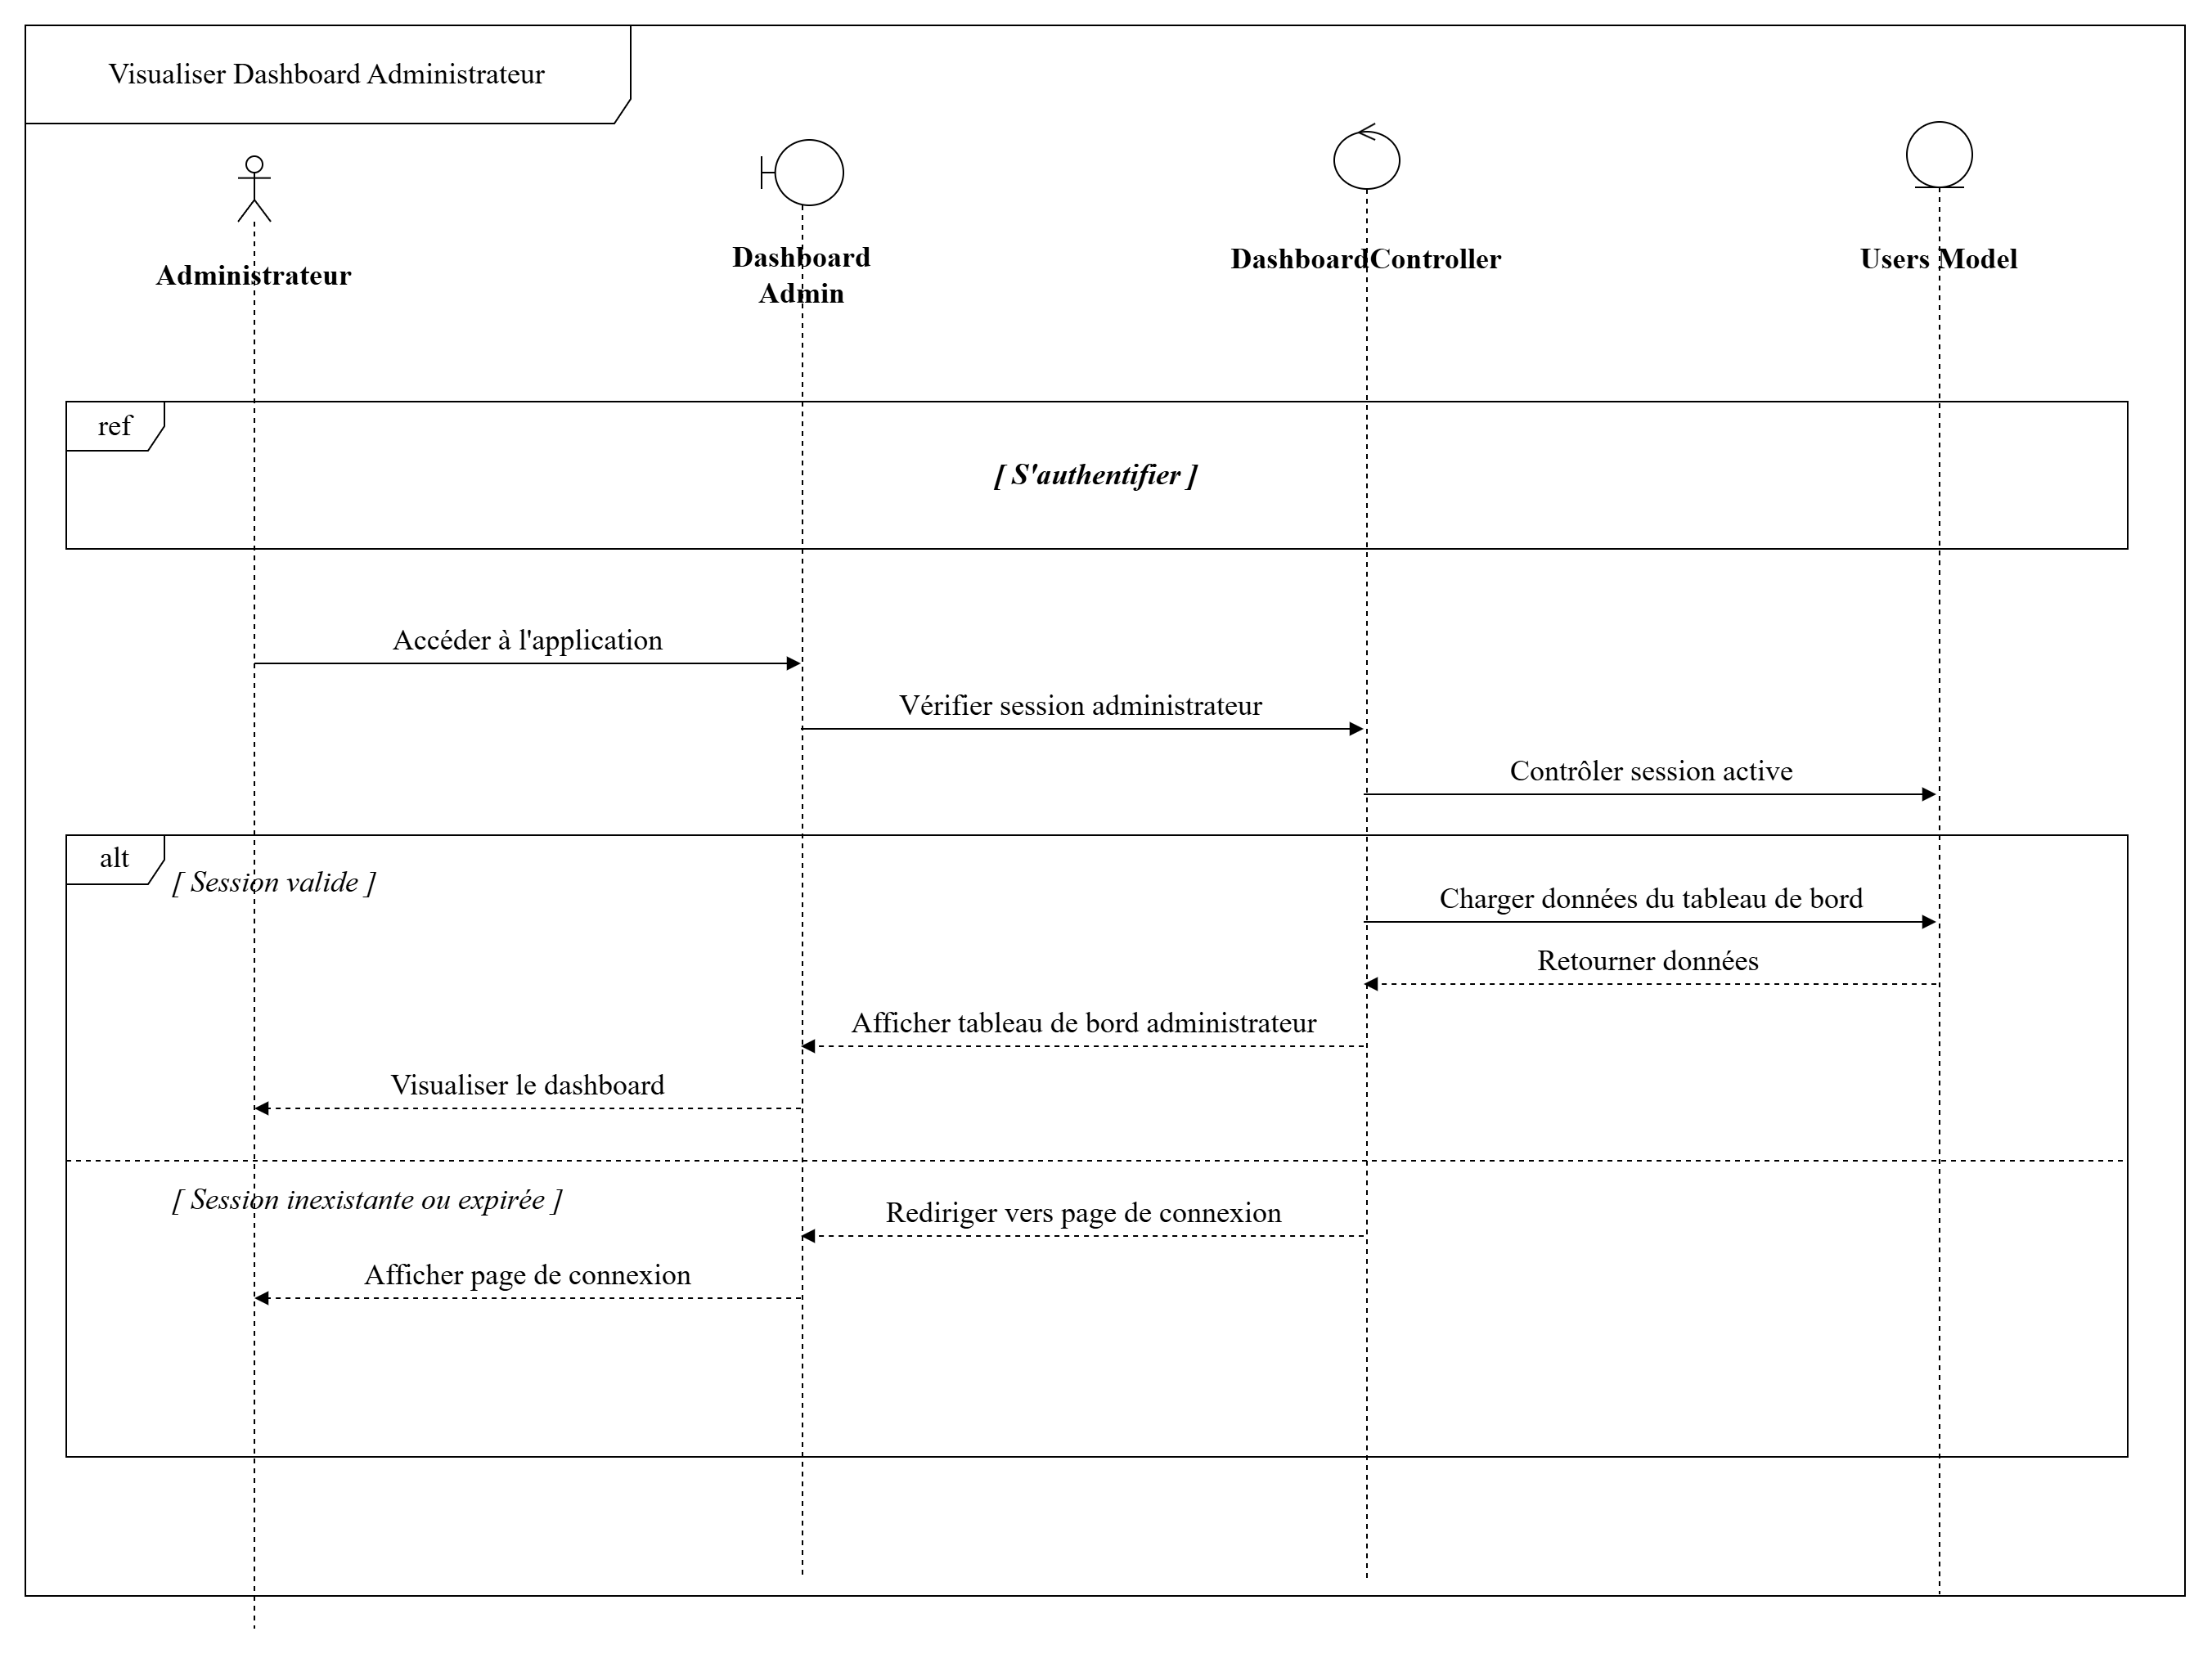
\includegraphics[width=0.9\textwidth]{projet/images/sequence s4/dachbordad.drawio.png}
    \caption{Diagramme de séquence du cas d'utilisation «~Visualiser le Dashboard (Responsable Administrateur )»}
\end{figure}

\item[$\bullet$] \textbf{Diagramme de séquence du cas d'utilisation «~Visualiser le Dashboard (Responsable RH)~»}



\begin{figure}[H]
    \centering
    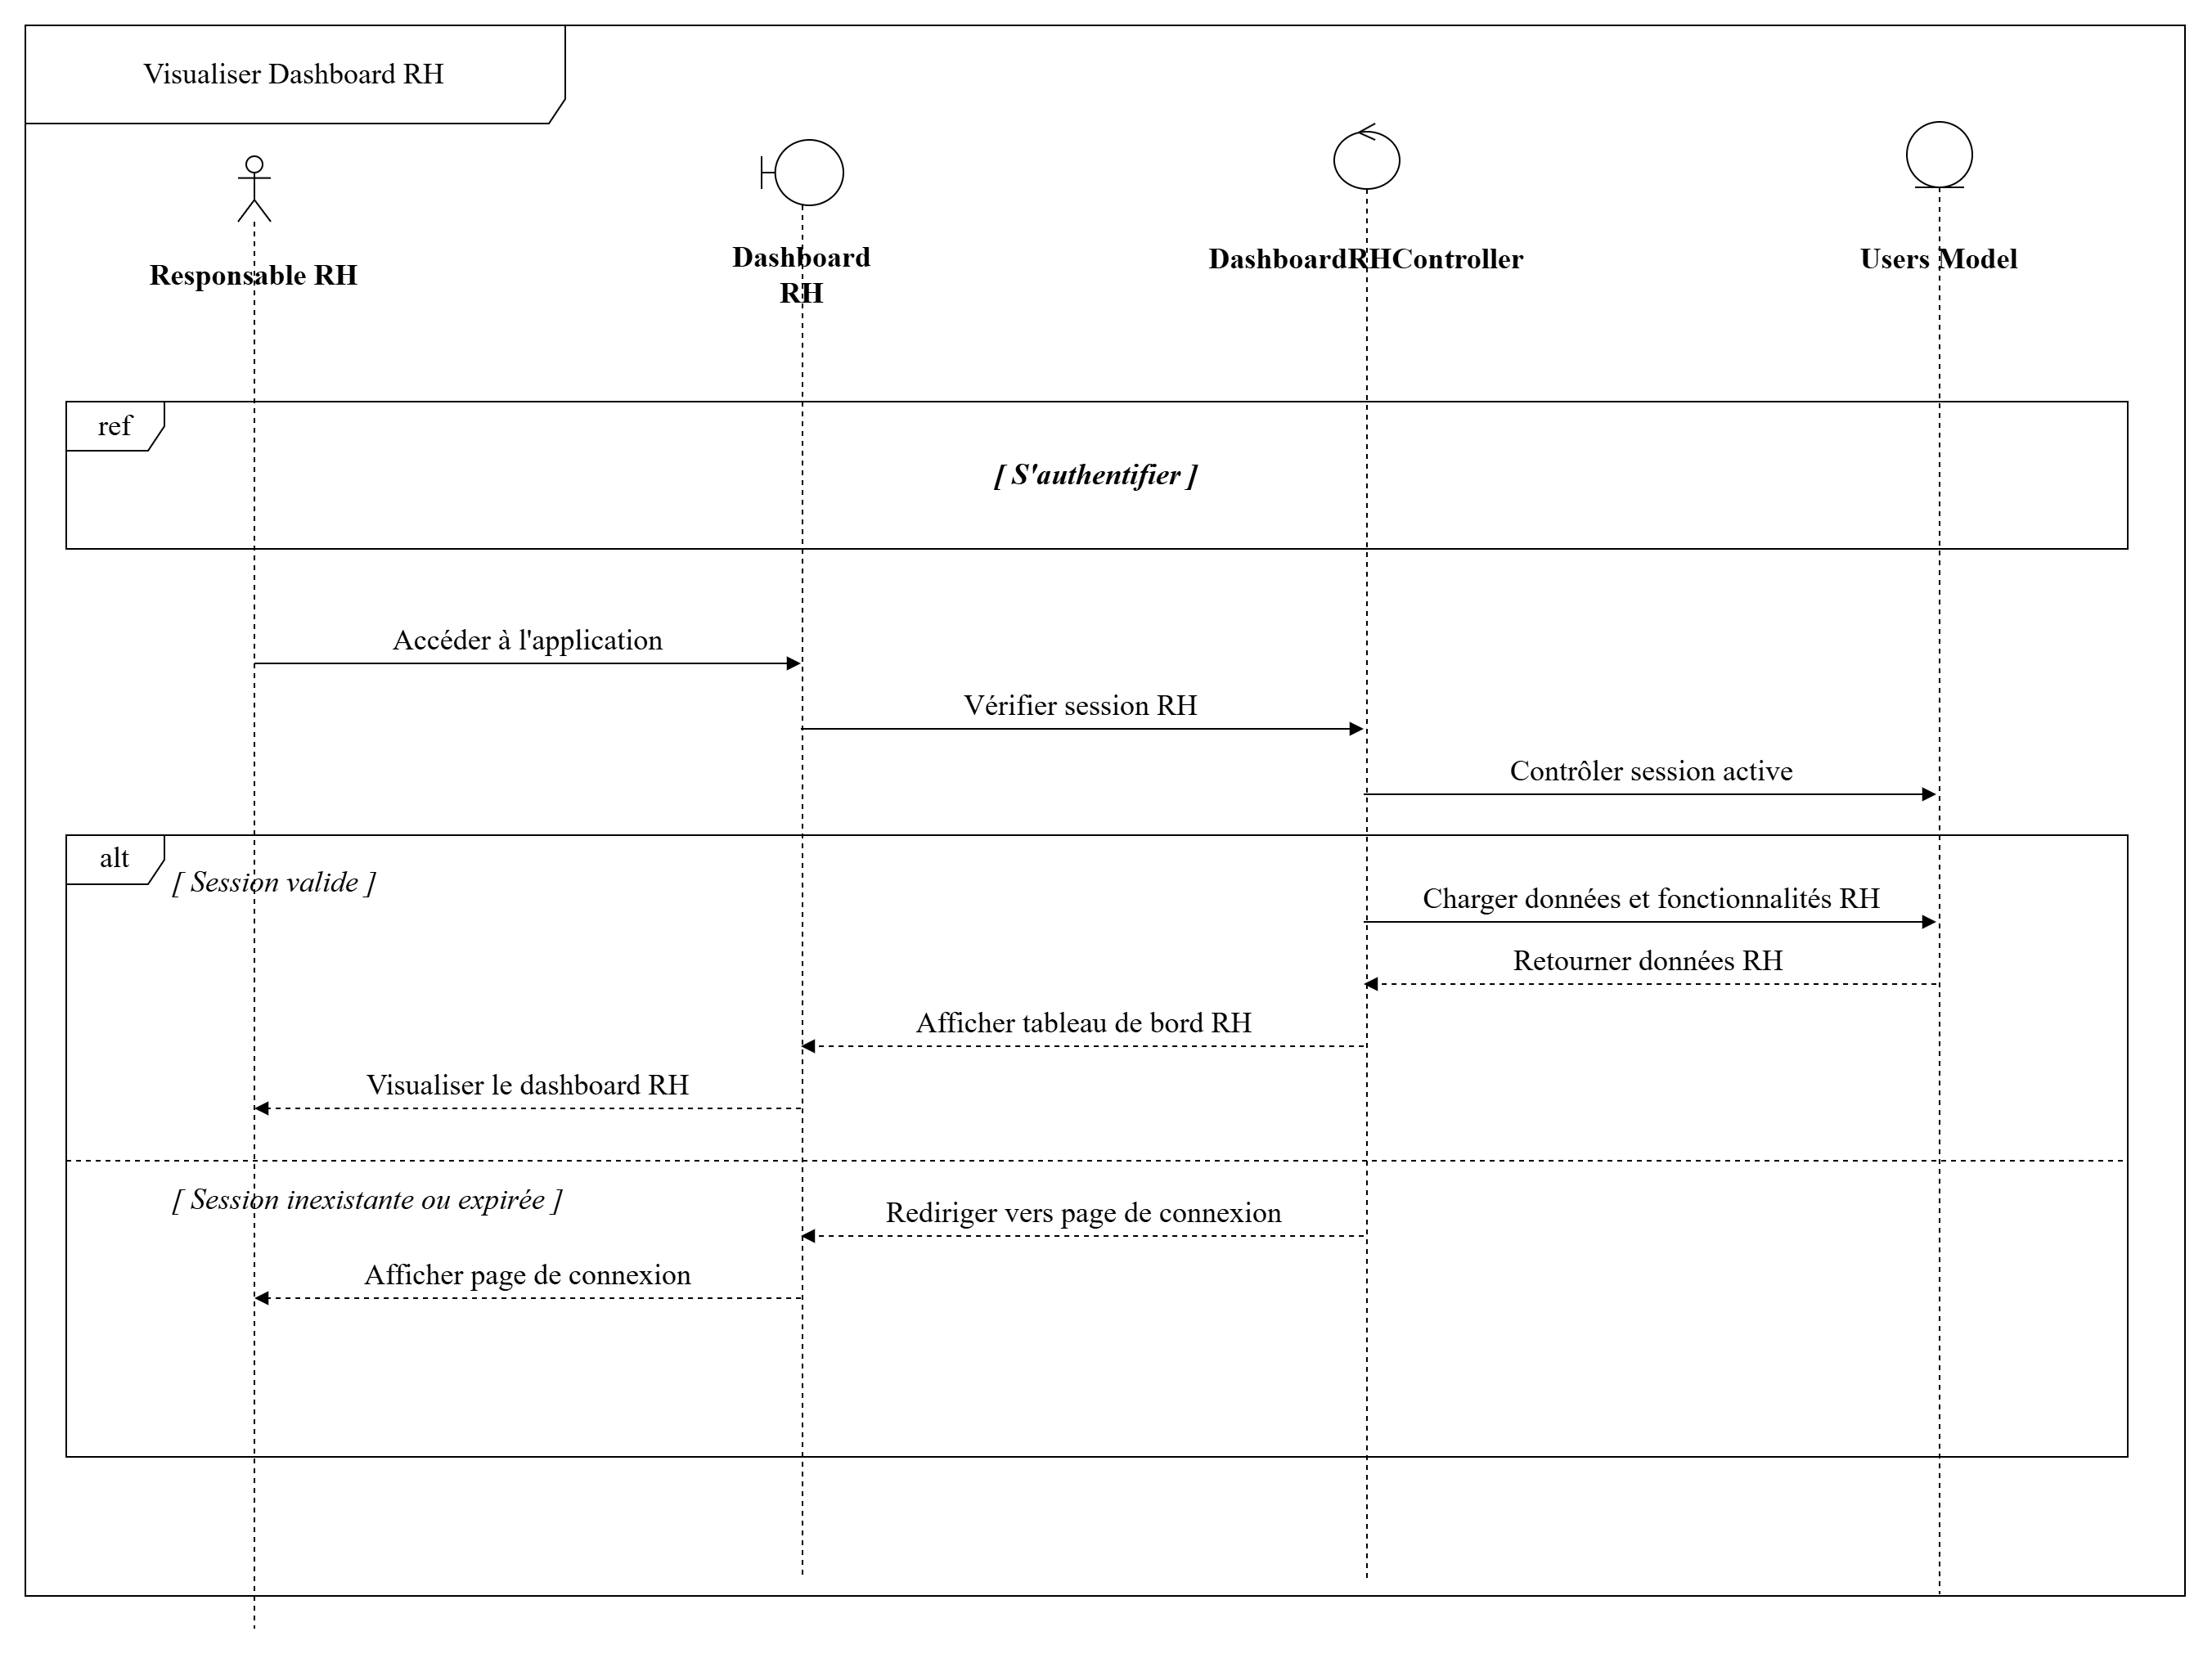
\includegraphics[width=0.9\textwidth]{projet/images/sequence s4/bash rh.drawio.png}
    \caption{Diagramme de séquence du cas d'utilisation «~Visualiser le Dashboard (Responsable RH)~»}
\end{figure}


\item[$\bullet$] \textbf{Diagramme de séquence du cas d'utilisation «Consulter historique »}



\begin{figure}[H]
    \centering
    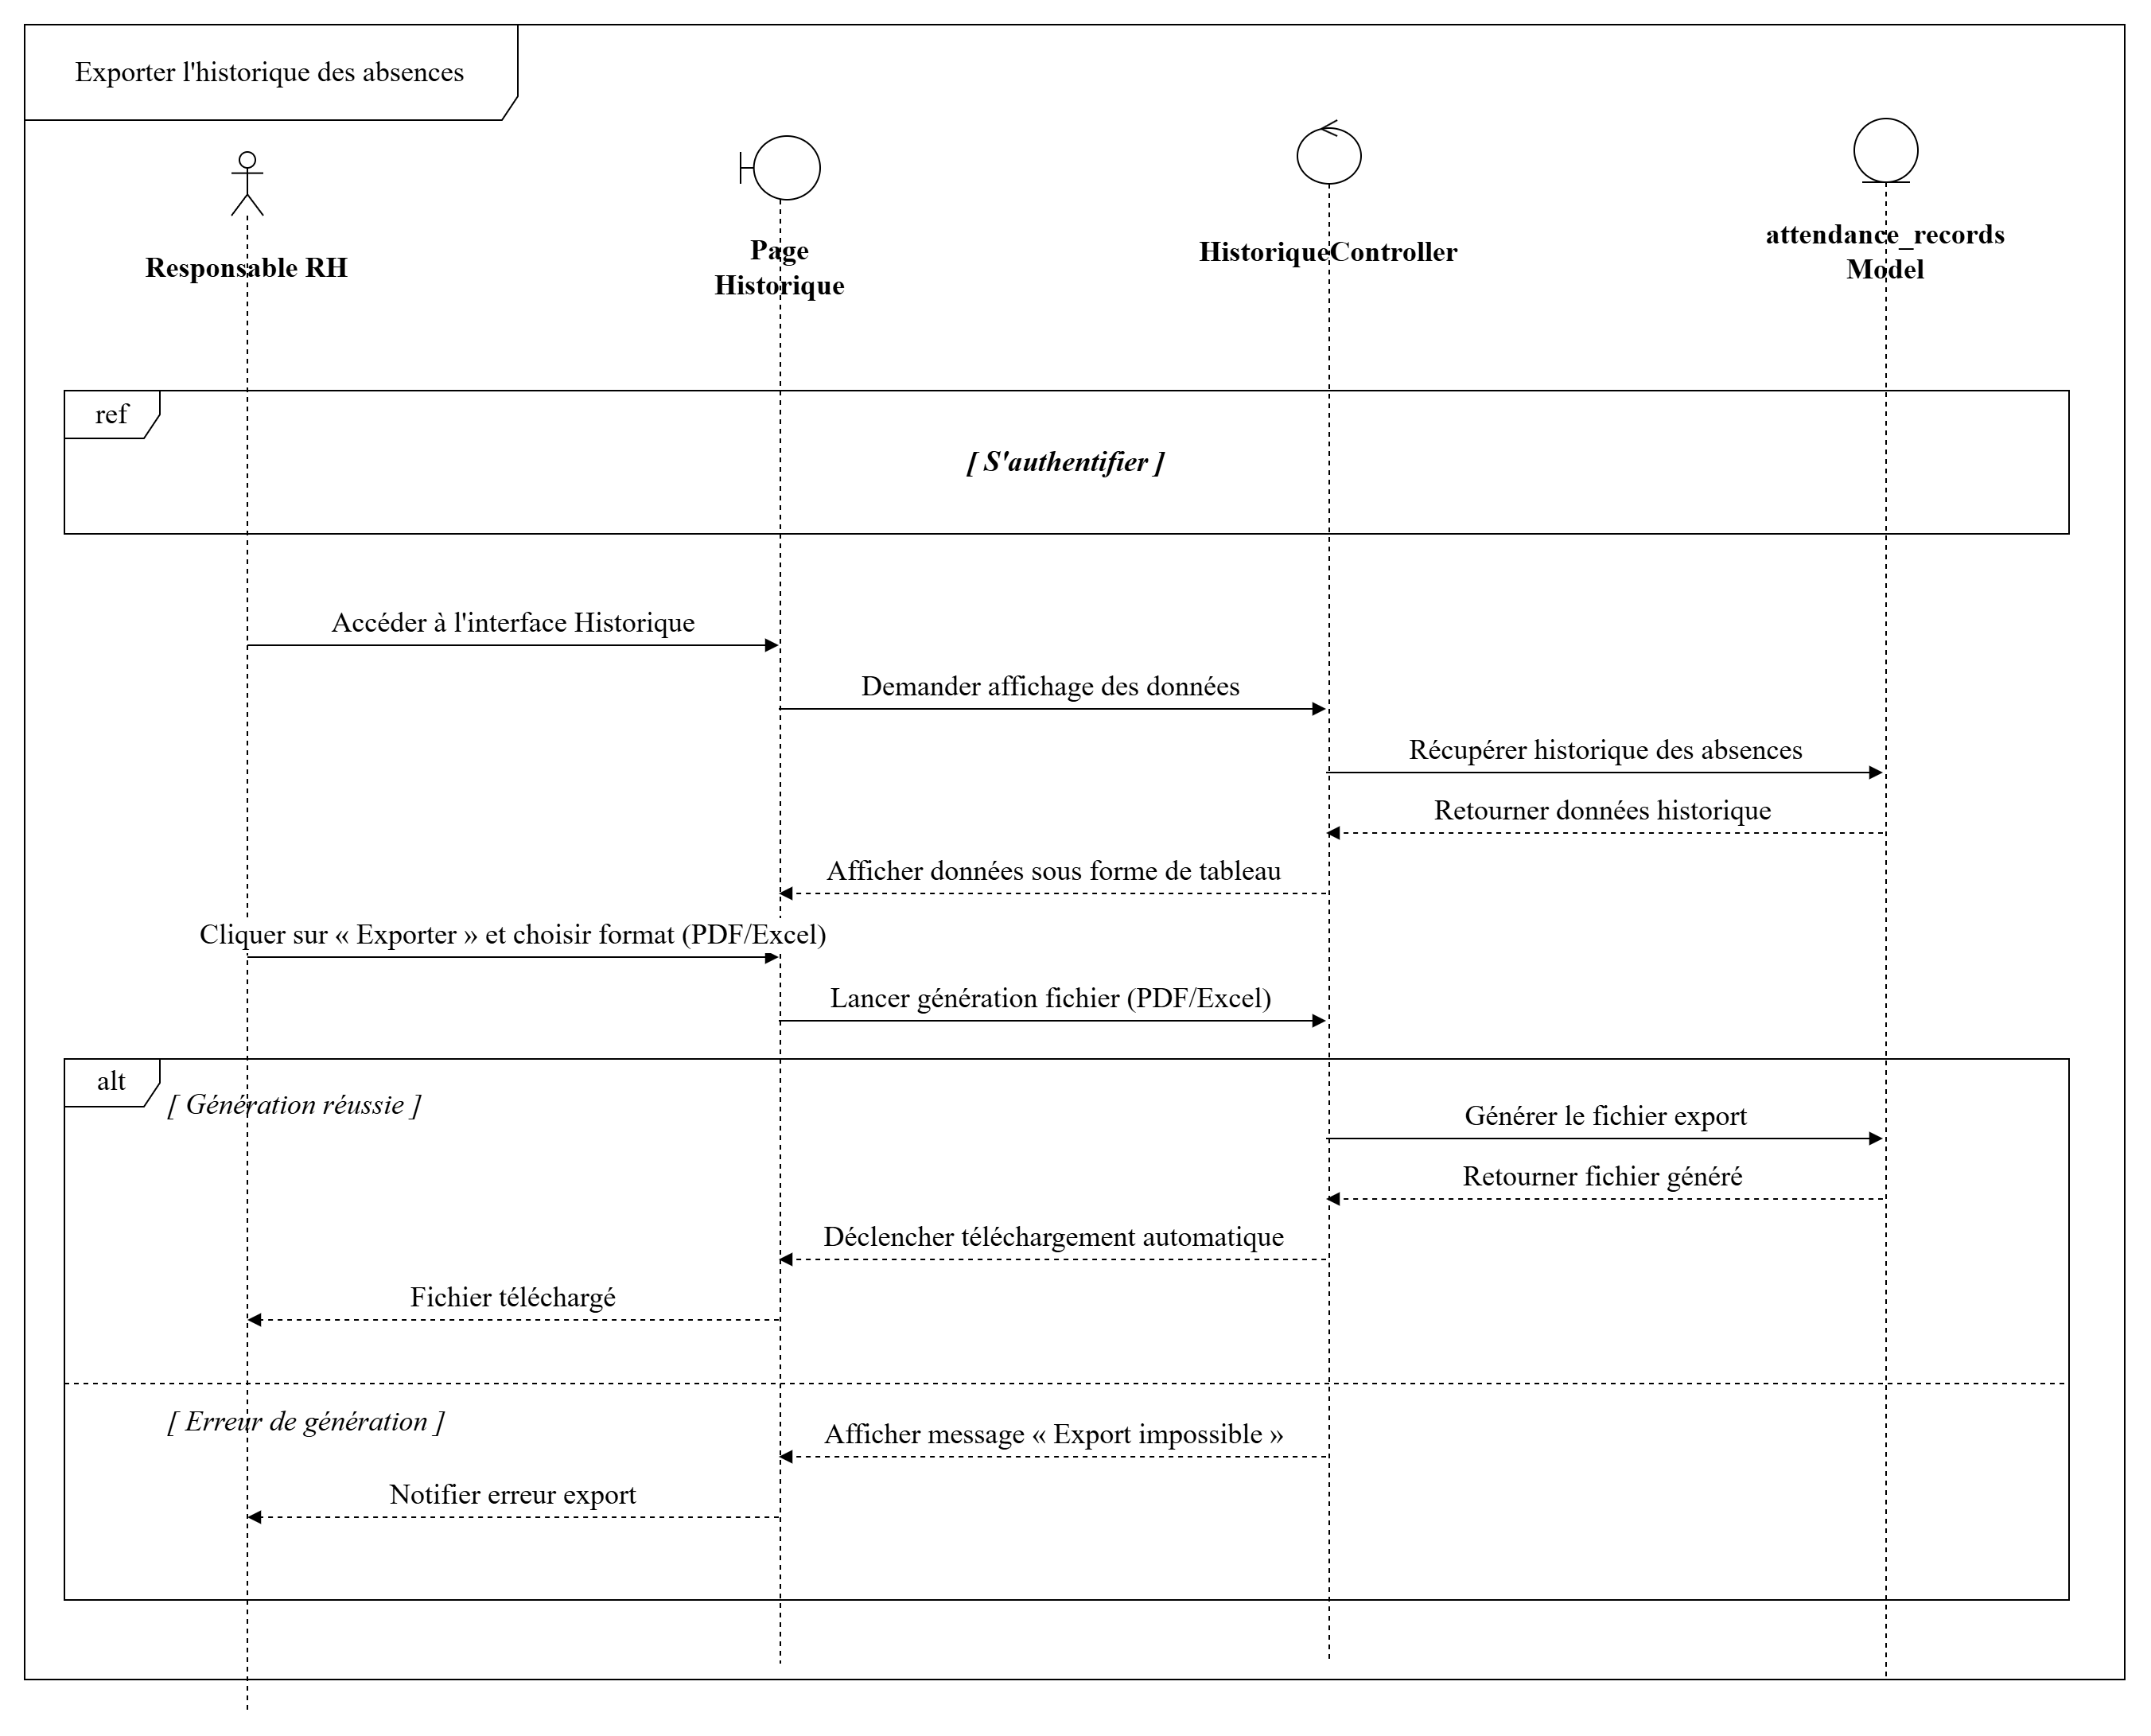
\includegraphics[width=0.9\textwidth]{projet/images/sequence s4/c historique.drawio.png}
    \caption{Diagramme de séquence du cas d'utilisation «~Consulter historique~»}
\end{figure}

\item[$\bullet$] \textbf{Diagramme de séquence du cas d'utilisation «~Exporter rapport~»}



\begin{figure}[H]
    \centering
    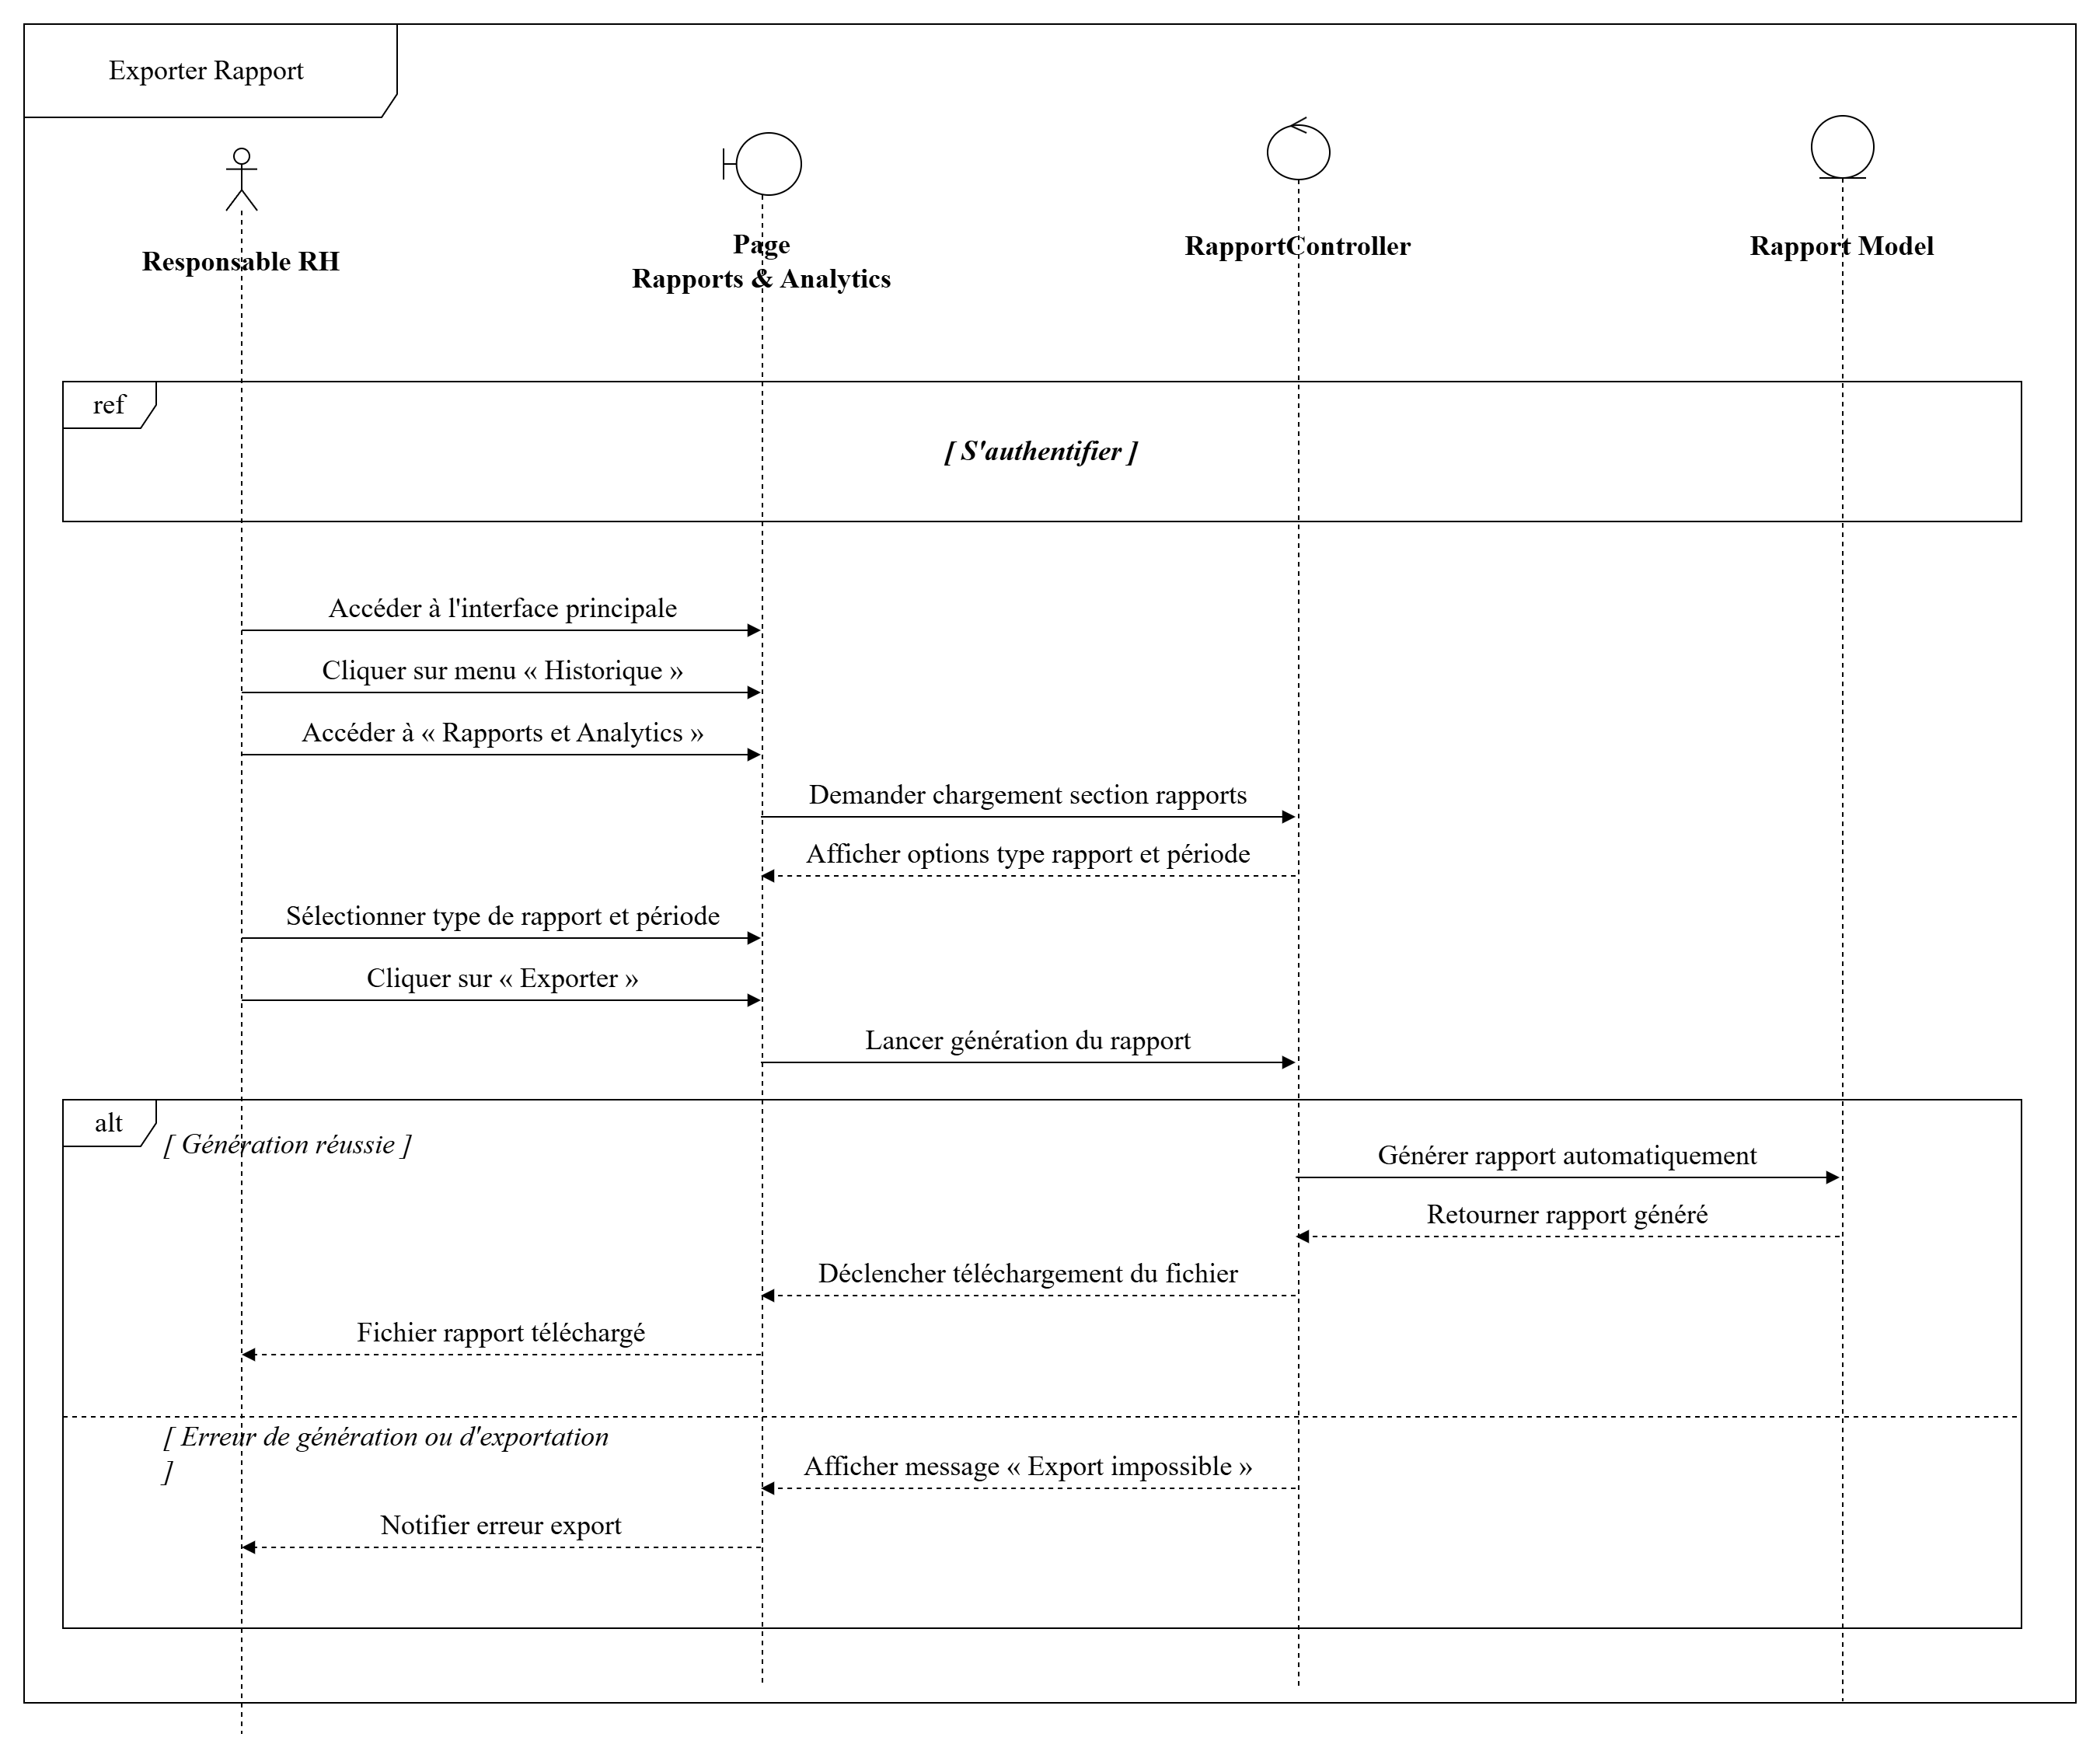
\includegraphics[width=0.9\textwidth]{projet/images/sequence s4/exporte.drawio.png}
    \caption{Diagramme de séquence du cas d'utilisation «~Exporter rapport~»}
\end{figure}

\end{itemize}

\subsection{Interfaces réalisées pour le sprint 4}

\begin{itemize}

\item[$\bullet$] \textbf{Dashboard Administrateur}

Cette page permet à l’administrateur de surveiller le fonctionnement global de la plateforme RH.  
Elle affiche les statistiques principales, les activités récentes et les informations importantes du système afin d’assurer une bonne gestion de la plateforme.

\begin{center}
    \begin{figure}[H]
        \centering
        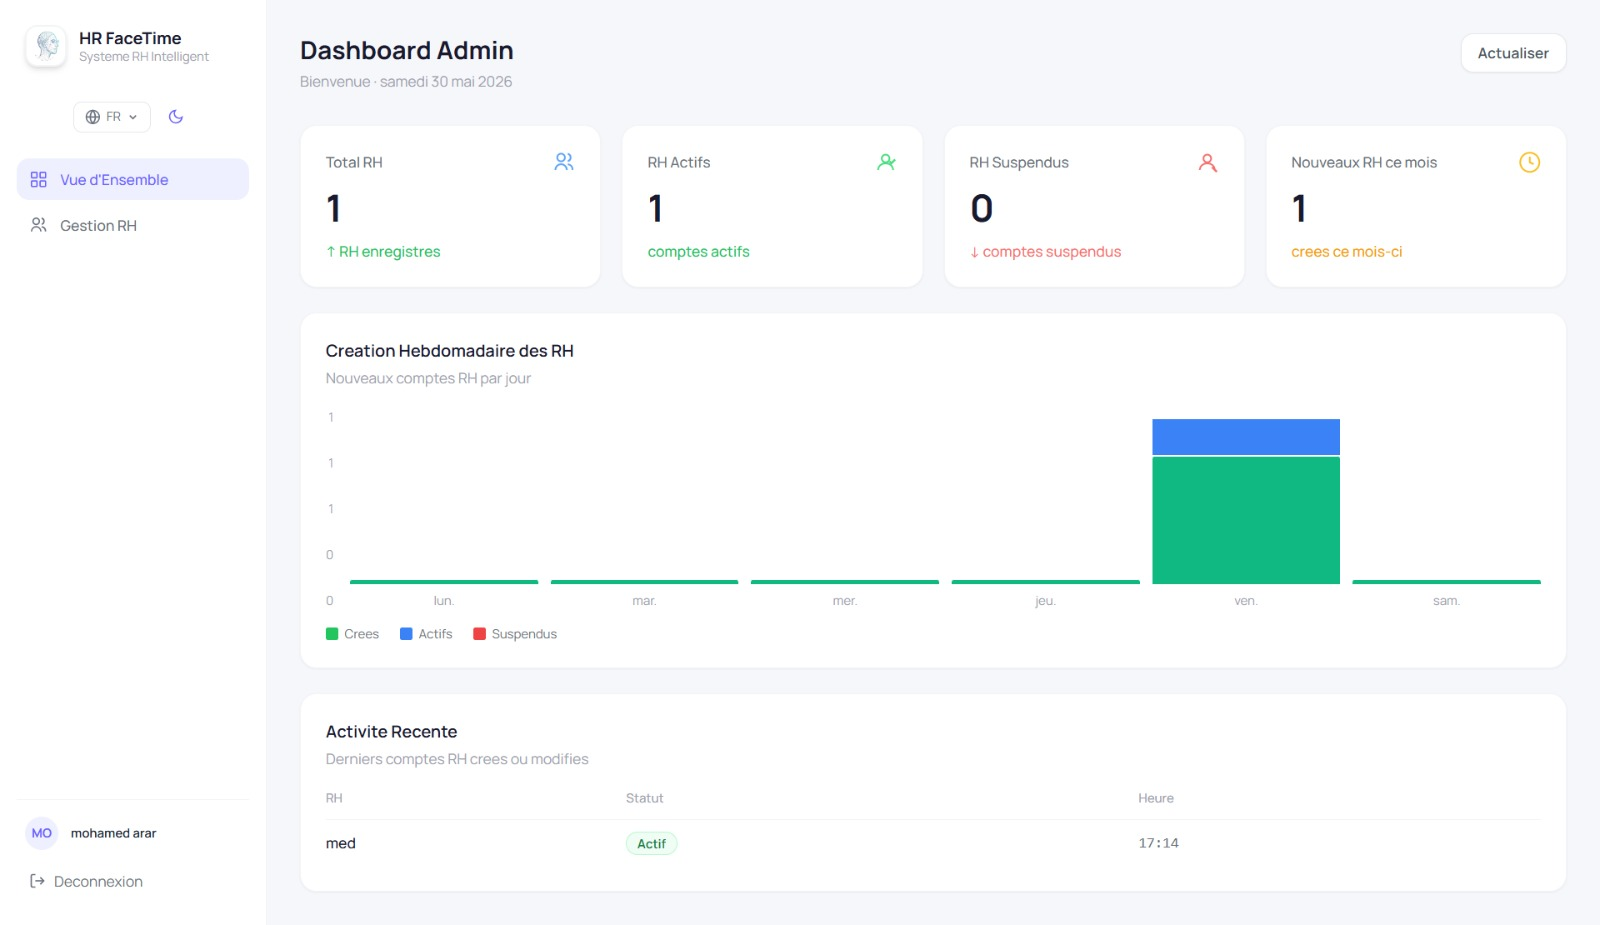
\includegraphics[width=0.9\textwidth]{projet/images/interface/s4/dashbord_admin.jpg}
        \caption{Interface du Dashboard Administrateur}
    \end{figure}
\end{center}

\item[$\bullet$] \textbf{Dashboard Responsable RH}

Cette page permet au responsable RH de visualiser les indicateurs liés aux employés, aux absences, aux congés et aux salaires.  
Elle facilite le suivi et le pilotage des activités RH de l’entreprise.

\begin{center}
    \begin{figure}[H]
        \centering
        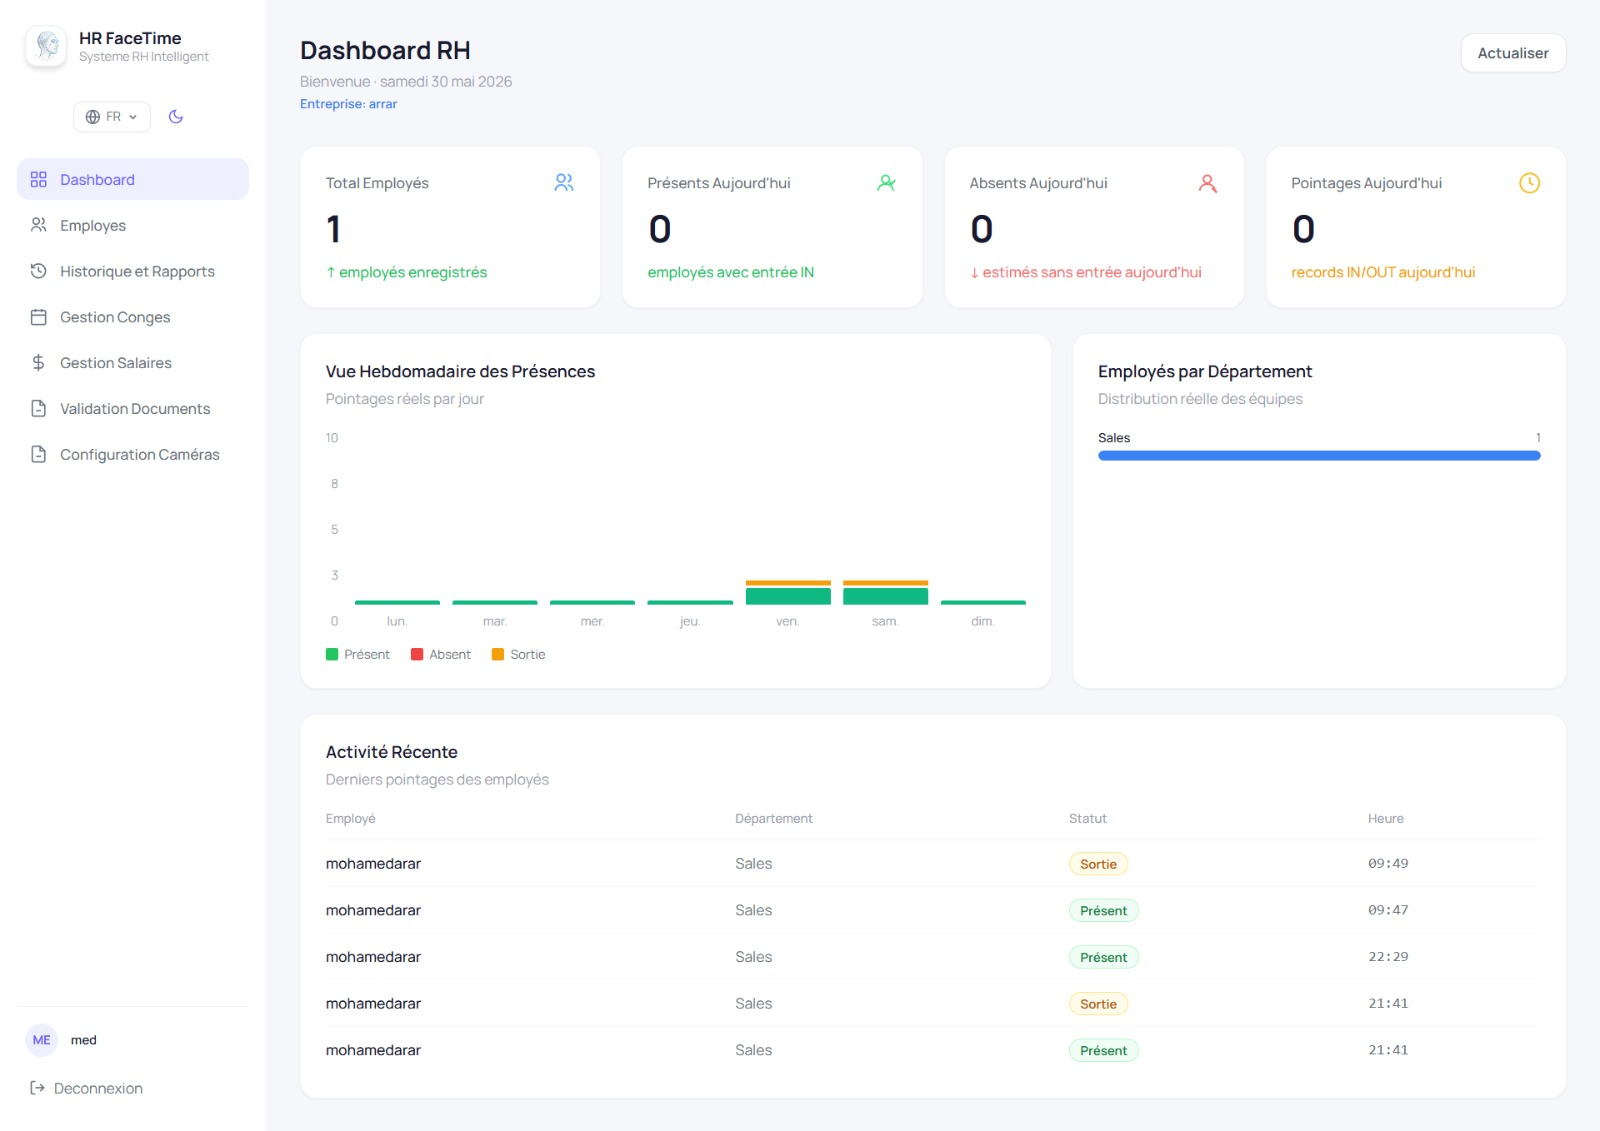
\includegraphics[width=0.9\textwidth]{projet/images/interface/s4/rh.jpeg}
        \caption{Interface du Dashboard Responsable RH}
    \end{figure}
\end{center}

\item[$\bullet$] \textbf{Exportation des Rapports}

Cette page permet de générer et télécharger différents rapports RH sous plusieurs formats.  
Elle aide à analyser les données administratives et à produire des documents de suivi.

\begin{center}
    \begin{figure}[H]
        \centering
        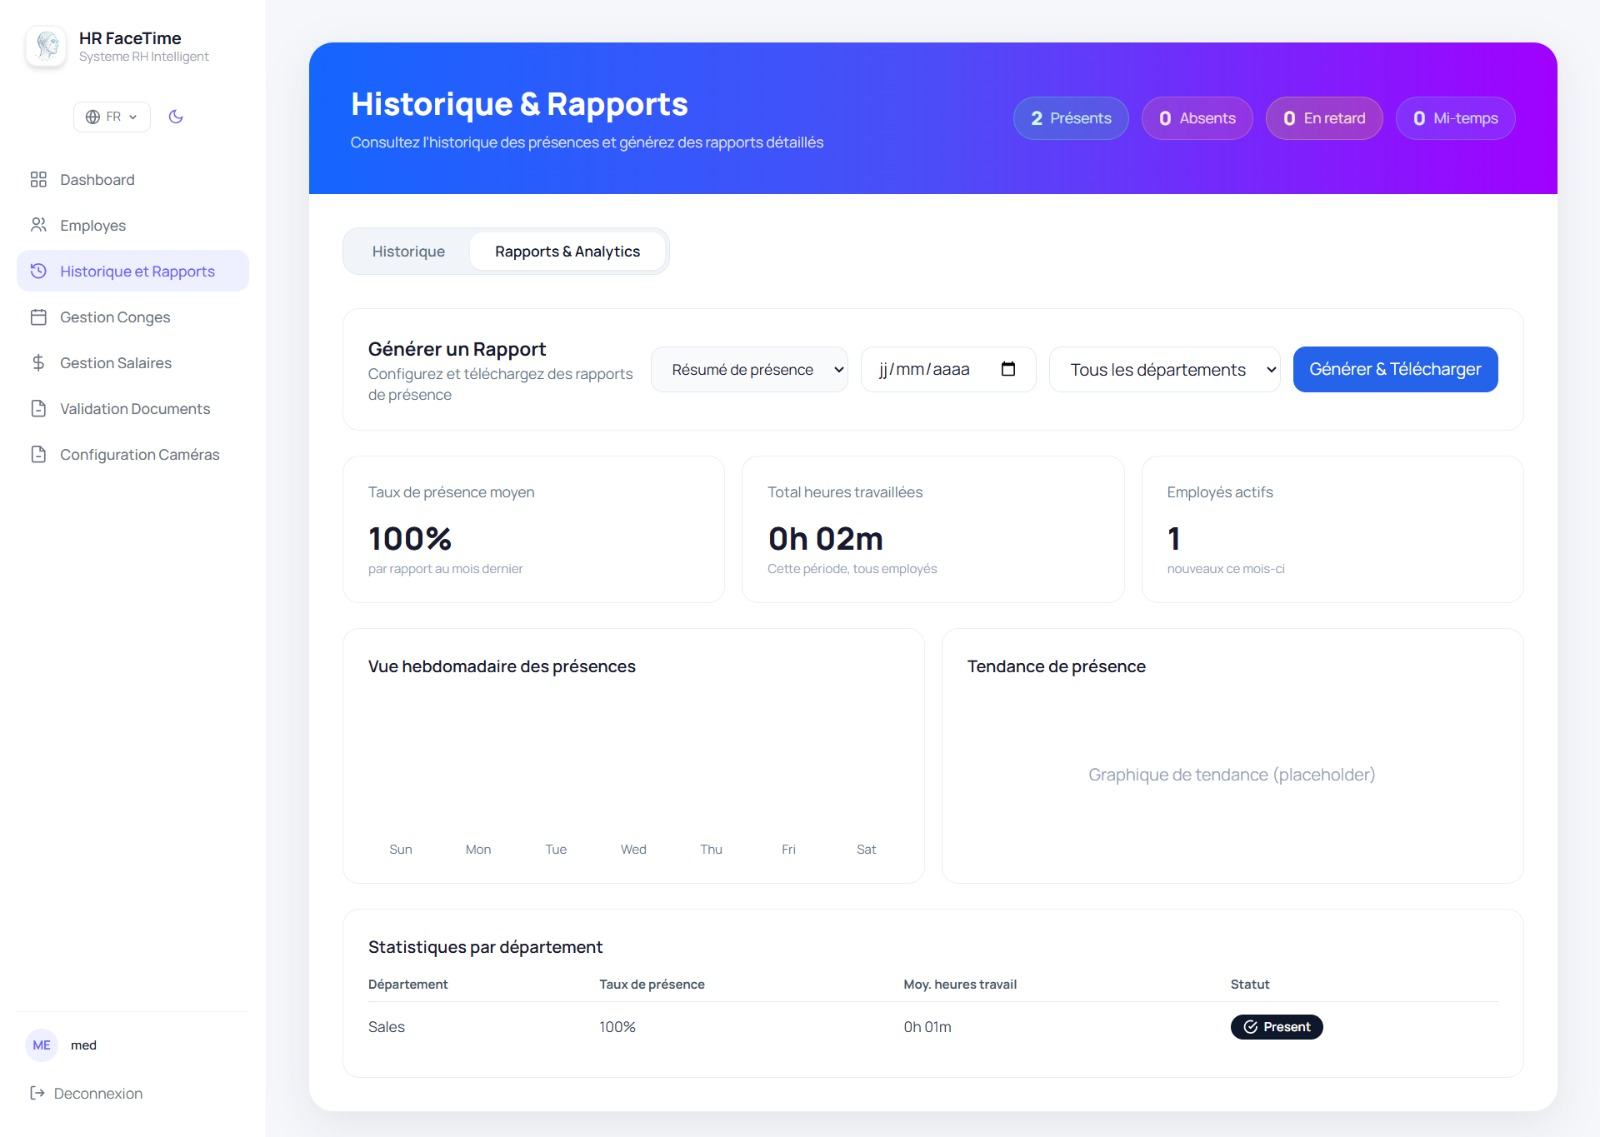
\includegraphics[width=0.9\textwidth]{projet/images/interface/s4/rapport.jpg}
        \caption{Interface d'exportation des rapports}
    \end{figure}
\end{center}


\item[$\bullet$] \textbf{ Consulter historique }

Cette page permet de consulter l’historique des actions effectuées sur la plateforme RH.  
Elle assure la traçabilité et le suivi des opérations réalisées par les utilisateurs.

\begin{center}
    \begin{figure}[H]
        \centering
        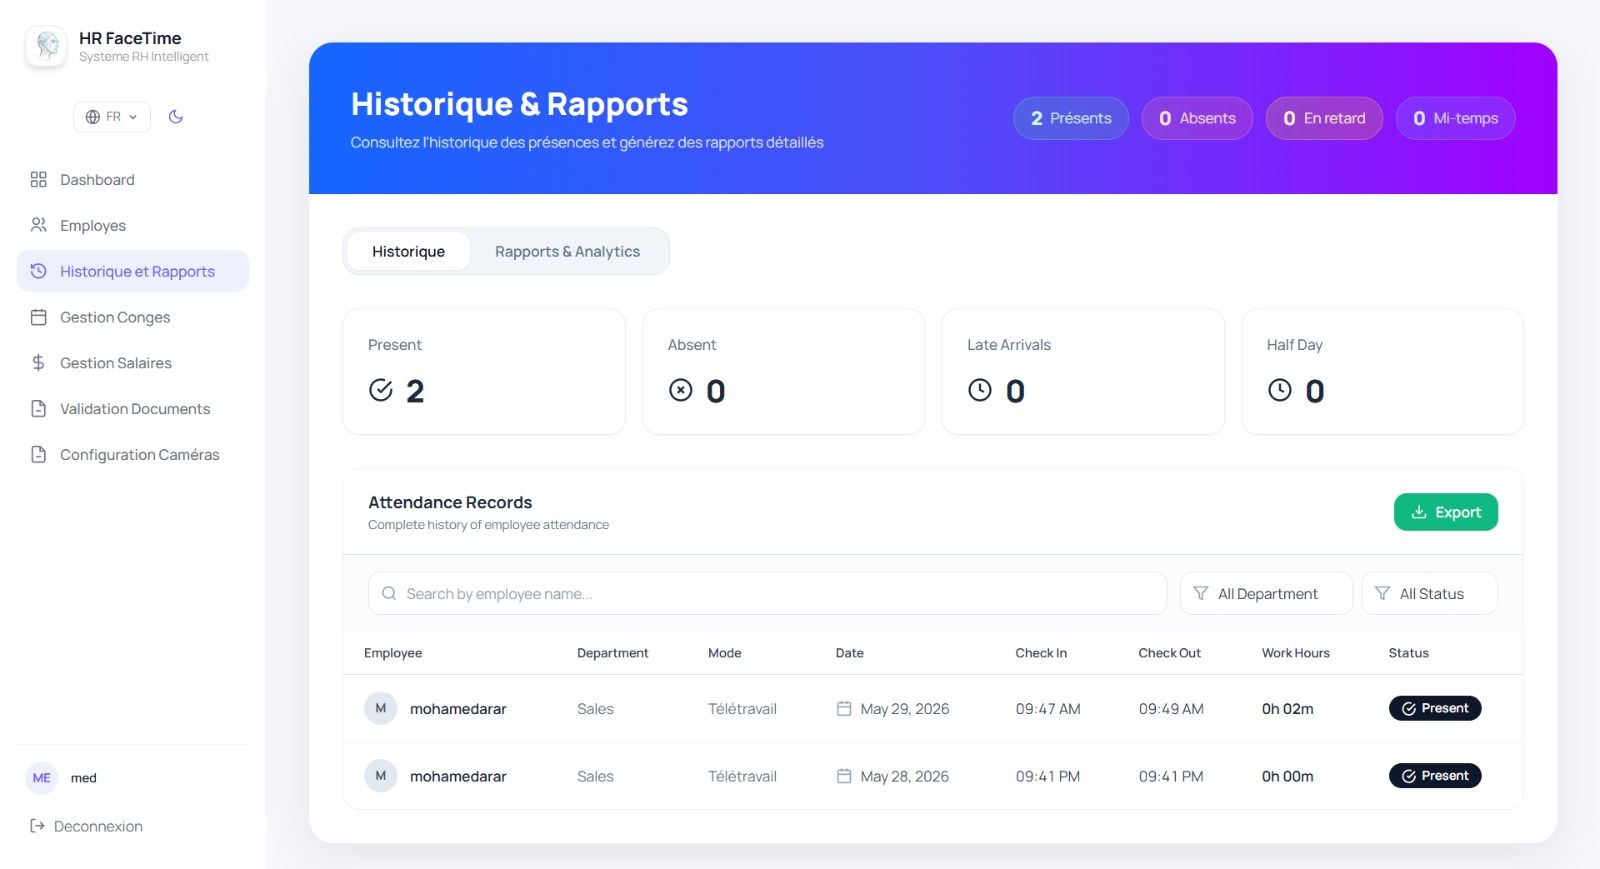
\includegraphics[width=0.9\textwidth]{projet/images/interface/s4/historique.jpg}
        \caption{Interface de Consulter historique}
    \end{figure}
\end{center}

\end{itemize}

\section{Conclusion}
Dans ce chapitre, nous avons présenté les livraisons des sprints 3 et 4, correspondant à la Release 2 du projet. Les fonctionnalités de gestion RH (congés, documents, primes, salaires) ainsi que les modules de statistiques, rapports et abonnement ont été détaillés à travers les backlog, spécifications fonctionnelles, conceptions et interfaces réalisées. Cette release constitue le produit final fonctionnel et complet du projet.